% !TeX encoding = UTF-8
% !TeX spellcheck = en_US

\newcommand{\doublequotes}[1]{``#1''}
\newcommand{\reference}[1]{\ref{#1} \nameref{#1} (page \pageref{#1})}
\newcommand{\introreference}[1]{Chapter \ref{#1}: \nameref{#1} (page \pageref{#1})}

\documentclass[a4paper,twoside]{report}

\pdfminorversion=7
\pdfcompresslevel=9
\pdfobjcompresslevel=2

\usepackage[hidelinks]{hyperref}
\usepackage[margin=60pt]{geometry}
\usepackage[T1]{fontenc}
\usepackage[utf8]{inputenc}
\usepackage[english]{babel}
\usepackage{array}
\usepackage{colortbl}
\usepackage{enumitem}
\usepackage{fancyhdr}
\usepackage{graphicx}
\usepackage{minted}
\usepackage{xcolor}

\usemintedstyle{staroffice}

\arrayrulecolor{lightgray}
\def\arraystretch{1.2}

\setlength{\parindent}{0pt}

\hypersetup{
    pdftitle={eMall - e-Mobility for All (RASD)},
    pdfauthor={Riccardo Motta and Pierluigi Negro}
}

\newcommand\nbvspace[1][3]{\vspace*{\stretch{#1}}}

\newcounter{goals}
\newcounter{worldphenomena}
\newcounter{sharedphenomena}
\newcounter{scenarios}
\newcounter{domainassumptions}
\newcounter{requirements}
\newcounter{usecases}

\setcounter{goals}{0}
\setcounter{worldphenomena}{0}
\setcounter{sharedphenomena}{0}
\setcounter{scenarios}{0}
\setcounter{domainassumptions}{0}
\setcounter{requirements}{0}
\setcounter{usecases}{0}

\newcommand{\showG}[1]{\refstepcounter{goals}\label{#1}G\thegoals}
\newcommand{\showWP}[1]{\refstepcounter{worldphenomena}\label{#1}WP\theworldphenomena}
\newcommand{\showSP}[1]{\refstepcounter{sharedphenomena}\label{#1}SP\thesharedphenomena}
\newcommand{\showS}[1]{\refstepcounter{scenarios}\label{#1}S\thescenarios}
\newcommand{\showD}[1]{\refstepcounter{domainassumptions}\label{#1}D\thedomainassumptions}
\newcommand{\showR}[1]{\refstepcounter{requirements}\label{#1}R\therequirements}
\newcommand{\showUC}[1]{\refstepcounter{usecases}\label{#1}UC\theusecases}

\newcommand{\refG}[1]{G\ref{#1}}
\newcommand{\refWP}[1]{WP\ref{#1}}
\newcommand{\refSP}[1]{SP\ref{#1}}
\newcommand{\refS}[1]{S\ref{#1}}
\newcommand{\refD}[1]{D\ref{#1}}
\newcommand{\refR}[1]{R\ref{#1}}
\newcommand{\refUC}[1]{UC\ref{#1}}

\raggedbottom

\renewcommand{\headrulewidth}{0pt}

\fancypagestyle{plain}{
    \fancyhead{}
    \fancyfoot{}
    \fancyfoot[LE,RO]{\thepage}
}

\pagestyle{fancy}

\fancyhead{}
\fancyfoot{}

\renewcommand{\chaptermark}[1]{\markboth{#1}{#1}}

\fancyhead[RO,LE]{\textcolor{gray}{\if\thechapter0{\contentsname}\else\chaptername\ \thechapter:\ \leftmark\fi}}
\fancyfoot[LE,RO]{\thepage}

\begin{document}

    \begin{titlepage}

        \begin{center}

            \nbvspace[1]

            
\includegraphics[width=0.3\columnwidth]{./images/polimi}

            \nbvspace[2]

            {\huge \textbf{\textsc{eMall - e-Mobility for All}}} \\
            [1.5em]
            {\Large \textbf{R}equirements \textbf{A}nalysis and \textbf{S}pecification \textbf{D}ocument}

            \nbvspace[6]

            \Large \textbf{Riccardo Motta \\ Pierluigi Negro}

            \nbvspace[2]

            \today \\ [0.5em]
            Version 1.1

            \nbvspace[1]

        \end{center}

    \end{titlepage}

    \tableofcontents{}

    \chapter{Introduction} \label{introduction}

Nowadays, electric vehicles are becoming very popular. The need to reduce pollution to save our planet is compelling, and anything we can do to reduce the effects of climate change is moving towards the use of clean energy sources, and everyone can do their part.\medskip

Many people are changing their cars to electric ones, and in many cities charging stations are being installed for these vehicles. The main aim of the \textsc{eMall} project is to limit the carbon footprint of our mobility by making easy and efficient charging electric cars, focusing on planning the charge.\medskip

The \textsc{eMall} project also focuses on the energy needed to accomplish charging cars, as it's important to manage it most efficiently. This is done to reduce the cost of the primary resources and to make the service even more competitive and cheap. The \textsc{eMall} project tries to simplify also this aspect of the charge chain.

\section{Purpose}

The purpose of this document is to provide a general, complete, high-level view of the eMSP and CPMS systems, and of their interactions.\medskip

This document comprehends:
\begin{itemize}
    \item The description of the main goals of the project, with the identification of the interesting phenomena. These phenomena are selected among the ones that might indirectly influence the system or that the system has knowledge of.
    \item The main scenarios the system can handle. Each of them is then precisely depicted more formally thanks to the use of diagrams.
    \item The system's requirements.
    \item A formal analysis of the requirements' feasibility.
\end{itemize}

\section{Scope}

\paragraph{eMSP | Simplify the charging process of electric vehicles} Charging an electric vehicle can be a challenging task to do. Nowadays, it's not so easy to find charging stations where to plug the vehicle. So, also looking at the future where this kind of station will be more present in the territory, it's fundamental to have a system like this one to carefully plan the charge of the vehicle, in order to minimize the time spent on this task, so that it doesn't have any impact on drivers' lives. Thanks to this system it's possible to search for a charging station nearby, check prices and sales, and, of course, book a charging slot for the vehicle.

\paragraph{CPMS | Optimize the energy usage and supply} To be competitive, it's also important to minimize the costs of the whole infrastructure, paying careful attention to the price of the electricity and to the mix of primary sources from which it was derived. On the market, there are possibly many DSOs, each one with different supply capabilities, prices, and energy mixes. Choosing from which source to buy the energy is crucial, especially if the CPO can store it in batteries at the charging station.

\pagebreak

\section{Goals}

More formally, here are formalized all the goals that the system should archive.

\subsection{eMSP goals}

This first part focuses on the goals related to the eMPS.

\begin{center}
    \begin{tabular}{ >{\arraybackslash}m{0.06\columnwidth} | >{\arraybackslash}m{0.88\columnwidth} }
        \textbf{\showG{g:e:lookup}} & \textbf{Allow the user to see all the charging stations} \\
        \hline
        \multicolumn{2}{p{0.966\columnwidth}}{
            The user can see and look for all the available charging stations with all the important information, like the cost of the charge and any special offers.
        } \\
    \end{tabular}
\end{center}
\begin{center}
    \begin{tabular}{ >{\arraybackslash}m{0.06\columnwidth} | >{\arraybackslash}m{0.88\columnwidth} }
        \textbf{\showG{g:e:book}} & \textbf{Allow the user to book a charge} \\
        \hline
        \multicolumn{2}{p{0.966\columnwidth}}{
            Every user can reserve a charge if any slot is available. The user can select a charging station, the starting time, and the duration of the charge. Moreover, s/he selects the type of socket to use.
        } \\
    \end{tabular}
\end{center}
\begin{center}
    \begin{tabular}{ >{\arraybackslash}m{0.06\columnwidth} | >{\arraybackslash}m{0.88\columnwidth} }
        \textbf{\showG{g:e:start}} & \textbf{Allow the user to start the charge} \\
        \hline
        \multicolumn{2}{p{0.966\columnwidth}}{
            Every user who has booked can start the charging process during the booked period. This is done automatically by recognizing the connected vehicle once the socket is plugged in.
        } \\
    \end{tabular}
\end{center}
\begin{center}
    \begin{tabular}{ >{\arraybackslash}m{0.06\columnwidth} | >{\arraybackslash}m{0.88\columnwidth} }
        \textbf{\showG{g:e:notify}} & \textbf{Let the system notify the user when the charge is finished} \\
        \hline
        \multicolumn{2}{p{0.966\columnwidth}}{
            End users are informed every time one of their vehicles charging in one station ends the recharging process through a notification.
        } \\
    \end{tabular}
\end{center}
\begin{center}
    \begin{tabular}{ >{\arraybackslash}m{0.06\columnwidth} | >{\arraybackslash}m{0.88\columnwidth} }
        \textbf{\showG{g:e:pay}} & \textbf{Allow the user to pay for the service} \\
        \hline
        \multicolumn{2}{p{0.966\columnwidth}}{
            Every user can pay for the obtained charging process.
        } \\
    \end{tabular}
\end{center}

\subsection{CPMS goals}

This second part, instead, focuses on the goals related to the CPMS.

\begin{center}
    \begin{tabular}{ >{\arraybackslash}m{0.06\columnwidth} | >{\arraybackslash}m{0.88\columnwidth} }
        \textbf{\showG{g:c:info}} & \textbf{Let the system have information about charging stations} \\
        \hline
        \multicolumn{2}{p{0.966\columnwidth}}{
            Know the position and the characteristics of all the various charging stations, like sockets, batteries, available energy, and occupation.
        } \\
    \end{tabular}
\end{center}
\begin{center}
    \begin{tabular}{ >{\arraybackslash}m{0.06\columnwidth} | >{\arraybackslash}m{0.88\columnwidth} }
        \textbf{\showG{g:c:charge}} & \textbf{Allow for cars to charge} \\
        \hline
        \multicolumn{2}{p{0.966\columnwidth}}{
            Start the charge of a vehicle, monitoring the process.
        } \\
    \end{tabular}
\end{center}
\begin{center}
    \begin{tabular}{ >{\arraybackslash}m{0.06\columnwidth} | >{\arraybackslash}m{0.88\columnwidth} }
        \textbf{\showG{g:c:dso}} & \textbf{Fetch information from DSO and decide which DSO to use} \\
        \hline
        \multicolumn{2}{p{0.966\columnwidth}}{
            Acquire the price of the electricity from the providers and decide from which to buy, if more options are available. 
        } \\
    \end{tabular}
\end{center}
\begin{center}
    \begin{tabular}{ >{\arraybackslash}m{0.06\columnwidth} | >{\arraybackslash}m{0.88\columnwidth} }
        \textbf{\showG{g:c:mix}} & \textbf{Define energy mix} \\
        \hline
        \multicolumn{2}{p{0.966\columnwidth}}{
            Decide the mix of electricity to provide to the sockets, deciding whether to buy energy, use the one stored in batteries or buy energy to store in batteries.
        } \\
    \end{tabular}
\end{center}
\begin{center}
    \begin{tabular}{ >{\arraybackslash}m{0.06\columnwidth} | >{\arraybackslash}m{0.88\columnwidth} }
        \textbf{\showG{g:c:offers}} & \textbf{Manage special offers} \\
        \hline
        \multicolumn{2}{p{0.966\columnwidth}}{
            Create new special offers on prices for charging.
        } \\
    \end{tabular}
\end{center}

\pagebreak

\section{Phenomena}

This part focuses on the description of the various interesting phenomena that are important in order to correctly develop this project.

\subsection{World phenomena}

World phenomena are the ones that are proper of the world's domain, and therefore invisible to the modeled machine, but still, it's important to point them out since they influence the system.

\begin{center}
    \begin{tabular}{ | >{\centering\arraybackslash}m{0.1\columnwidth} | >{\arraybackslash}m{0.84\columnwidth} | }
        \hline
        \textbf{Identifier} & \multicolumn{1}{c|}{\textbf{Description}} \\
        \hline
        \hline
        \showWP{wp:lookup} & The user looks for a nearby station (with its cost and offers). \\
        \hline
        \showWP{wp:vehicle} & The user brings the vehicle to the charging column for the booked charging slot. \\
        \hline
    \end{tabular}
\end{center}

\subsection{Shared phenomena}

This first part points out the shared phenomena between the world and the machine that are world-controlled.

\begin{center}
    \begin{tabular}{ | >{\centering\arraybackslash}m{0.1\columnwidth} | >{\arraybackslash}m{0.84\columnwidth} | }
        \hline
        \textbf{Identifier} & \multicolumn{1}{c|}{\textbf{Description}} \\
        \hline
        \hline
        \showSP{sp:w:book} & The user books a charging slot in a charging station. \\
        \hline
        \showSP{sp:w:plugin} & The user plugs in the vehicle for the charge. \\
        \hline
        \showSP{sp:w:unplug} & The user unplugs the vehicle after the charge or to stop it. \\
        \hline
        \showSP{sp:w:pay} & The user pays for the obtained service. \\
        \hline
        \showSP{sp:w:dso} & The DSO changes the price of the electricity. \\
        \hline
        \showSP{sp:w:energy} & The electricity for charging the vehicles is provided. \\
        \hline
    \end{tabular}
\end{center}

This second part, instead, focuses on the machine-controlled shared phenomena.

\begin{center}
    \begin{tabular}{ | >{\centering\arraybackslash}m{0.1\columnwidth} | >{\arraybackslash}m{0.84\columnwidth} | }
        \hline
        \textbf{Identifier} & \multicolumn{1}{c|}{\textbf{Description}} \\
        \hline
        \hline
        \showSP{sp:m:start} & The system starts the charge of a vehicle. \\
        \hline
        \showSP{sp:m:notify} & The system notifies the user when the charging process is finished. \\
        \hline
        \showSP{sp:m:batteries} & The system changes the charging level of the batteries, storing or consuming their energy. \\
        \hline
        \showSP{sp:m:distribution} & The system manages the distribution of energy to the vehicles. \\
        \hline
        \showSP{sp:m:price} & The system acquires information about the current price of the energy offered by DSOs. \\
        \hline
    \end{tabular}
\end{center}

Moreover, some shared phenomena can be both world-controlled and machine-controlled. These are listed down here.

\begin{center}
    \begin{tabular}{ | >{\centering\arraybackslash}m{0.1\columnwidth} | >{\arraybackslash}m{0.84\columnwidth} | }
        \hline
        \textbf{Identifier} & \multicolumn{1}{c|}{\textbf{Description}} \\
        \hline
        \hline
        \showSP{sp:cost} & The cost of a charge is changed. \\
        \hline
        \showSP{sp:offer} & A special offer is added or removed. \\
        \hline
        \showSP{sp:mix} & The energy mix for a specific vehicle is decided. \\
        \hline
        \showSP{sp:battery} & The decision whether to use the battery energy or to store it in one is taken by the user. \\
        \hline
        \showSP{sp:dso} & The decision of the DSO from which buying the energy is taken by the user. \\
        \hline
    \end{tabular}
\end{center}

\pagebreak

\section{Definitions, acronyms and abbreviations}

\subsection{Definitions}

\begin{center}
    \begin{tabular}{ | >{\centering\arraybackslash}m{0.15\columnwidth} | >{\arraybackslash}m{0.79\columnwidth} | }
        \hline
        \textbf{Word} & \multicolumn{1}{c|}{\textbf{Definition}} \\
        \hline
        \hline
        eRoaming & The \textit{eRoaming} is an external service that the system can query in order to obtain information about the various connected eMPSs and CPMSs. \\
        \hline
    \end{tabular}
\end{center}

\subsection{Acronyms}

\begin{center}
    \begin{tabular}{ | >{\centering\arraybackslash}m{0.15\columnwidth} | >{\arraybackslash}m{0.79\columnwidth} | }
        \hline
        \textbf{Acronym} & \multicolumn{1}{c|}{\textbf{Description}} \\
        \hline
        \hline
        API & \textit{Application Programming Interface}: is a set of instructions and interfaces that is standardized in order to facilitate the communication between different pieces of software. \\
        \hline
        CPMS & \textit{Charge Point Management System}: the CPOs management system that supports the process of charging vehicles and acquiring energy from the various DSOs. \\
        \hline
        CPO & \textit{Charging Point Operator}: the name of the operators managing the charging points and providing the actual charging service. \\
        \hline
        DBMS & \textit{DataBase Management System}: it's the system that sits between the physical data structures on disk and the user, allowing to create, read, update and delete data. \\
        \hline
        DSO & \textit{Distribution System Operator}: the name of the operators that provide the actual energy used during the charging process. \\
        \hline
        eMSP & \textit{e-Mobility Service Provider}: the name of the providers of the service to the end users, acting as intermediaries between the users and the backing CPOs. \\
        \hline
        ES6 & \textit{ECMAScript 6}: is a JavaScript standard which ensures interoperatibility between different web browsers. \\
        \hline
        JWT & \textit{JSON Web Token}: is a standardized method for securely representing claims between two parties. \\
        \hline
        UML & \textit{Unified Modeling Language}: is a modeling language used to formally specify the design of a system. \\
        \hline
    \end{tabular}
\end{center}

\subsection{Abbreviations}

\begin{center}
    \begin{tabular}{ | >{\centering\arraybackslash}m{0.15\columnwidth} | >{\arraybackslash}m{0.79\columnwidth} | }
        \hline
        \textbf{Abbreviation} & \multicolumn{1}{c|}{\textbf{Description}} \\
        \hline
        \hline
        \textsc{eMall} & \textsc{eMall - e-Mobility for All}. \\
        \hline
    \end{tabular}
\end{center}

\section{Revision history}

\paragraph{Version 1.0} released on December 22, 2022: original release.
\paragraph{Version 1.1} released on \today: uniformed section names, fixed alloy worlds, updated \refUC{uc:e:book}, \refUC{uc:e:edit} and \refUC{uc:e:payment}, added \nameref{credits} section and fixed typos.

\section{Reference documents}

\begin{enumerate}
    \item \textbf{M. Camilli, E. Di Nitto, M. G. Rossi}; \textit{eMall - e-Mobility for All project} (2022)
\end{enumerate}

\pagebreak

\section{Document structure}

\paragraph{\introreference{introduction}} This first part provides a general introduction to the project and describes the main purpose and goals it tries to archive, defining the scope of the project and pointing out some definitions, acronyms, and abbreviations used in this document. Moreover, there are all the revisions of the document with all the references used for writing it.

\paragraph{\introreference{description}} This second part focuses on a formal description of the project, explaining all the possible scenarios in which the application is used. The formalization part in this section is done by taking advantage of various UML diagrams, which won't cover every possibility since, as stated in this chapter, some domain assumptions limit the scope. Furthermore, it's provided a brief but precise description of the characteristics of the various types of users, with their respective needs, that interact with the system.

\paragraph{\introreference{requirements}} This third part, instead, is concerned with all the specific requirements that can be useful when developing the system. In particular, are pointed out all the interfaces that should be present (user, hardware, software, and communication interfaces), together with functional and performance requirements. Also, there are some design constraints and all the reliability, availability, security, maintainability, and portability attributes of the system.

\paragraph{\introreference{alloy}} This fourth part covers the formal description of the whole system thanks to the use of a modeling language such as Alloy that allows proving the feasibility of the goals, starting from all the constraints and requirements.

\paragraph{\introreference{conclusions}} This last part contains the last notes about the project and concludes this document, pointing out the effort that each of the authors of this document spent in order to release it.

    \chapter{Overall Description} \label{description}

This chapter describes the whole system, focusing on use cases, scenarios, functionalities, domain assumptions, and users thanks to the use of formalization diagrams, like UML.

\section{Product perspective}

In this section are listed all the possible scenarios that the system should be able to handle, and there is also an overview of the class structure of the project that is used to accomplish these needs.

\subsection{Scenarios}

These first scenarios are seen from the point of view of the end user (consumer)\footnote{A precise description of the different types of users (consumer and CPO's) is provided in section \reference{users}.} who wants to charge the vehicle.

\begin{center}
    \begin{tabular}{ >{\arraybackslash}m{0.06\columnwidth} | >{\arraybackslash}m{0.88\columnwidth} }
        \textbf{\showS{s:e:registration}} & \textbf{Registration and setup} \\
        \hline
        \multicolumn{2}{p{0.966\columnwidth}}{
            Mathew Assafo has just bought a new electric car, but he finds out that there are only a few charging stations in the city where he lives. After talking to some friends that already bought an electric car, he finds out that there exists an eMSP service that allows one to search for charging stations and book a charge. So when he arrives back home, he decides to look into it. Once he finds the eMSP, he looks for the sign-up page and inserts all the required data. Once filled up, he receives an email containing a link for confirming the account. After having confirmed the address, he is redirected to the login page where he inserts his username (email address) and password. Since this is the first time he logs in, he is prompted to choose which one he prefers as the default method for receiving notifications. He can choose between receiving an in-app notification or an email. He chooses the first option and the system warns him that whenever the system cannot reach any logged-in device, that notification will be sent via email.
        } \\
        \hline
    \end{tabular}
\end{center}
\begin{center}
    \begin{tabular}{ >{\arraybackslash}m{0.06\columnwidth} | >{\arraybackslash}m{0.88\columnwidth} }
        \textbf{\showS{s:e:book}} & \textbf{Booking a charge} \\
        \hline
        \multicolumn{2}{p{0.966\columnwidth}}{
            Mathew Assafo has just completed the registration procedure and has already set up the application (he has set the preference for notifications). Now he can finally start planning his car's charges. First, he opens the vehicles section where he can insert all the data about his new electric car, then he opens the map to look for all the available charging stations. The system immediately asks him if he wants to enable the geolocalization of the device to easily see all the nearby stations. He grants permission and the map focuses on the surroundings of his house, finding out that there is a relatively near station that he has never seen before. He is happy since he doesn't have to move too much from home, making it not a problem if it rains or if it's cold. Furthermore, he clicks on the station icon to see all the details and to book the first charge. A popup appears showing him all the details of that charging station, including the 20\% discount on his first charge. Since it has few available slots, he presses on the booking button and selects an available slot of one hour for the next Sunday (while the vehicle to charge is already chosen by the system since it's the only available one). He already knows that next weekend he'll have to go with his wife to buy something for Christmas since it's already December, and they have no idea which gifts to buy for their children, so he decides that an extra charge to the vehicle would be worth it. He also marks the station as \doublequotes{favorite}, so that he'll be able to find it immediately next time. After he does this, a star appears in the corner of the map and on the charging station. Just to be sure, he clicks on the star on the map and finds out that the charging station he has just marked as \doublequotes{favorite} is there.
        } \\
        \hline
    \end{tabular}
\end{center}
\vfill
\begin{center}
    \begin{tabular}{ >{\arraybackslash}m{0.06\columnwidth} | >{\arraybackslash}m{0.88\columnwidth} }
        \textbf{\showS{s:e:edit}} & \textbf{Booking a charge and editing a reservation} \\
        \hline
        \multicolumn{2}{p{0.966\columnwidth}}{
            Mathew Assafo has just booked a charge for his vehicle in the charging station near his house. Since he needs his car also for going to work (lamentably, there are not so many public transport facilities where he lives) he clicks on the search bar and types in the address of his working place. Since there are a few stations near his workplace, he decides to switch from the map view to the list view, so that he can sort the results according to the price they offer, the distance from his workplace, and the general availability of the stations. After doing some tests, he finds out which station satisfies him. He marks it as \doublequotes{favorite} and books a few charges for the next few weeks. After booking these charges, he goes back to the home page where he finds a summary of all the future charges, in a list of cards with some brief details. He opens that section and scrolling down the list he realizes that the one he booked for Sunday coincides with a family meeting. So he clicks on the reservation and sees that, near the time section, there is an edit button (he also notices the red recycle bin on top, but he imagines that it'll probably delete the reservation). So he clicks on edit and a calendar with all the available slots (with the one he already booked that is marked) appears. He selects a previous slot so that the car will be fully charged before the family meeting and confirms.
        } \\
        \hline
    \end{tabular}
\end{center}
\begin{center}
    \begin{tabular}{ >{\arraybackslash}m{0.06\columnwidth} | >{\arraybackslash}m{0.88\columnwidth} }
        \textbf{\showS{s:e:start}} & \textbf{Start of charge} \\
        \hline
        \multicolumn{2}{p{0.966\columnwidth}}{
            It's Sunday morning, and Mathew Assafo wears his winter coat and brings the car to the charging station where he booked the charge. Before getting there, he receives a notification telling him the exact charging slot in which he has to park, so he stops there and connects the charging cable to the column. Immediately he notices that his car has started charging. He's surprised about the speed and how easy it is. Satisfied, he walks back home, in time for the start of the Formula 2 Grand Prix of that morning.
        } \\
        \hline
    \end{tabular}
\end{center}
\begin{center}
    \begin{tabular}{ >{\arraybackslash}m{0.06\columnwidth} | >{\arraybackslash}m{0.88\columnwidth} }
        \textbf{\showS{s:e:notification}} & \textbf{End-of-charge notification} \\
        \hline
        \multicolumn{2}{p{0.966\columnwidth}}{
            It's Sunday morning and Mathew Assafo is chilling on the sofa watching the Formula 2 Grand Prix. Suddenly his smartphone receives a notification. He gets up, takes the phone, and sees that the notification is from the eMSP application and is telling him that his vehicle has just finished charging. Even though he charged his car a couple of times during the previous working week, he is still surprised about the efficiency of the whole process. He takes his winter coat and goes to the charging station. He unplugs the vehicle and a notification immediately informs him that he can pay for the charge. He opens the application and clicks on the charge that is highlighted on the home page (the one he has to pay). When he starts the payment procedure in the application, he realizes that he doesn't remember some payment data, so he puts it back into his pocket and takes out his debit card. He goes near the charging column he used for charging the car and follows the instructions on the screen for paying the charge. Once done, he receives a notification of success, sits in his electric car, and goes back home, ready for the family meeting.
        } \\
        \hline
    \end{tabular}
\end{center}

The following scenarios are seen from the point of view of the CPO's authorized user who accesses the CPMS.

\begin{center}
    \begin{tabular}{ >{\arraybackslash}m{0.06\columnwidth} | >{\arraybackslash}m{0.88\columnwidth} }
        \textbf{\showS{s:c:dso}} & \textbf{Changing DSO} \\
        \hline
        \multicolumn{2}{p{0.966\columnwidth}}{
            Cameron Dya(z) is the owner of charging stations in the city of Paderno and discovers that, due to political allegations in the ongoing war, it would be beneficiary to the image of her company to not affiliate with DSOs owned by the attacking country, and decides to carry out the idea by changing DSOs provider. She turns on her computer, logs into the website of the CPMSs, heads to the section regarding the choice of the DSO, and clicks on \doublequotes{Deactivate automatic DSO choice}, then confirms the action. Afterward, she selects a new DSO from the ones operating in her city, making sure that the company of choice has nothing to do with the ongoing conflict. She once again confirms the action, logs out from the website, and turns off the computer, hoping that her actions will not be unnoticed.
        } \\
        \hline
    \end{tabular}
\end{center}
\begin{center}
    \begin{tabular}{ >{\arraybackslash}m{0.06\columnwidth} | >{\arraybackslash}m{0.88\columnwidth} }
        \textbf{\showS{s:c:mix1}} & \textbf{Changing the energy mix (case 1)} \\
        \hline
        \multicolumn{2}{p{0.966\columnwidth}}{
            The manager of the charging stations in Campobasso, Ahmed Ici, while listening to the weather forecast on the television, discovers that later that day, due to a downpour, the solar panels are not going to produce much energy. Knowing that without the help of the solar panels a lot of energy will be forcefully bought from the DSO, he opens his laptop and logs into the website of the CPMSs. He's in luck: by checking on the outgoing situation, he discovers that not a lot of cars are at the stations at the moment. This means that redirecting the energy produced by the solar panels to fill the station batteries will not have a huge impact in terms of costs. The batteries will help tamper with the absence of solar energy later that day, during the heavy rain, being a secondary source of the energy provided by the DSO. Hence, he goes to \doublequotes{Change energy mix}, and connects \doublequotes{solar panels} and \doublequotes{batteries}, effectively rerouting the energy flow. He confirms his choices and logs out of the website, knowing that once the batteries will be fully recharged the system will re-route the energy flow to a better usage of solar energy. 
        } \\
        \hline
    \end{tabular}
\end{center}
\begin{center}
    \begin{tabular}{ >{\arraybackslash}m{0.06\columnwidth} | >{\arraybackslash}m{0.88\columnwidth} }
        \textbf{\showS{s:c:mix2}} & \textbf{Changing the energy mix (case 2)} \\
        \hline
        \multicolumn{2}{p{0.966\columnwidth}}{
            To better combat battery aging, the CPO operator Joanna Sedini decides to let the batteries in the charging station that she manages discharge, seen as lately no cars bought a charge in the evening hours, and during the day the solar panels manage to cover the whole energy requirement. She, therefore, opens her laptop, logs into the website, and selects \doublequotes{Change energy mix}, connecting \doublequotes{Batteries} and \doublequotes{Outlet}. She then logs out and turns off her computer.
        } \\
        \hline
    \end{tabular}
\end{center}
\begin{center}
    \begin{tabular}{ >{\arraybackslash}m{0.06\columnwidth} | >{\arraybackslash}m{0.88\columnwidth} }
        \textbf{\showS{s:c:offer}} & \textbf{Adding a new special offer} \\
        \hline
        \multicolumn{2}{p{0.966\columnwidth}}{
            It's Christmastime, and the CPO CEO Carol Frat has a great idea: there should be a special Christmas offer for charges at her charging station. This will help persuade people to leave their electric cars charging while they go through their Christmas shopping spree, and maybe tempt other people into buying an electric car, seeing as charging it would come at a low price. Finalizing this idea is also fairly easy: she just goes into the website, logs in, selects \doublequotes{Create new special offer}, and inputs the parameters. She sets the starting date at the 8\textsuperscript{th} of December of the current year, the end date at the 6\textsuperscript{th} of January of next year, and the discount at 10\%.
        } \\
        \hline
    \end{tabular}
\end{center}
\begin{center}
    \begin{tabular}{ >{\arraybackslash}m{0.06\columnwidth} | >{\arraybackslash}m{0.88\columnwidth} }
        \textbf{\showS{s:c:crowd}} & \textbf{Monitoring of crowd situation at the stations} \\
        \hline
        \multicolumn{2}{p{0.966\columnwidth}}{
            Bruce He(l)m wants to renew one of his charging stations with a new set of batteries. Since all charging stations are similar in terms of battery status and performance comparisons, so he decides to play a quick game: he'll renew the most crowded station at the time of checking. So he opens a browser, goes to the website, and logs in. Then he proceeds to check the external situation of the stations one by one, and there is a single station currently winning the race: it's the only one with a lone car charging, all the others are empty! Unhappy with this result, he decides to change metric and looks for the station where the batteries are at their lowest charge. Funnily enough, the same station has a slightly lower percentage, so the decision can be easily taken.
        } \\
        \hline
    \end{tabular}
\end{center}

\subsection{Class diagram}

For graphical purposes, no attributes are shown and all the various handlers are not connected to all the components in the same package that uses it, but they are well integrated into the system. The same stands for the various APIs.\medskip

An example of this is the \texttt{PaymentService}. The \texttt{PaymentHandler} of the eMSP is the one that manages the transaction. It's connected to the \texttt{User} for getting data for notification, but also to \texttt{CPMShandler} since it has to notify the CPMS of the payment.

\begin{figure}[h!]
    \centering
    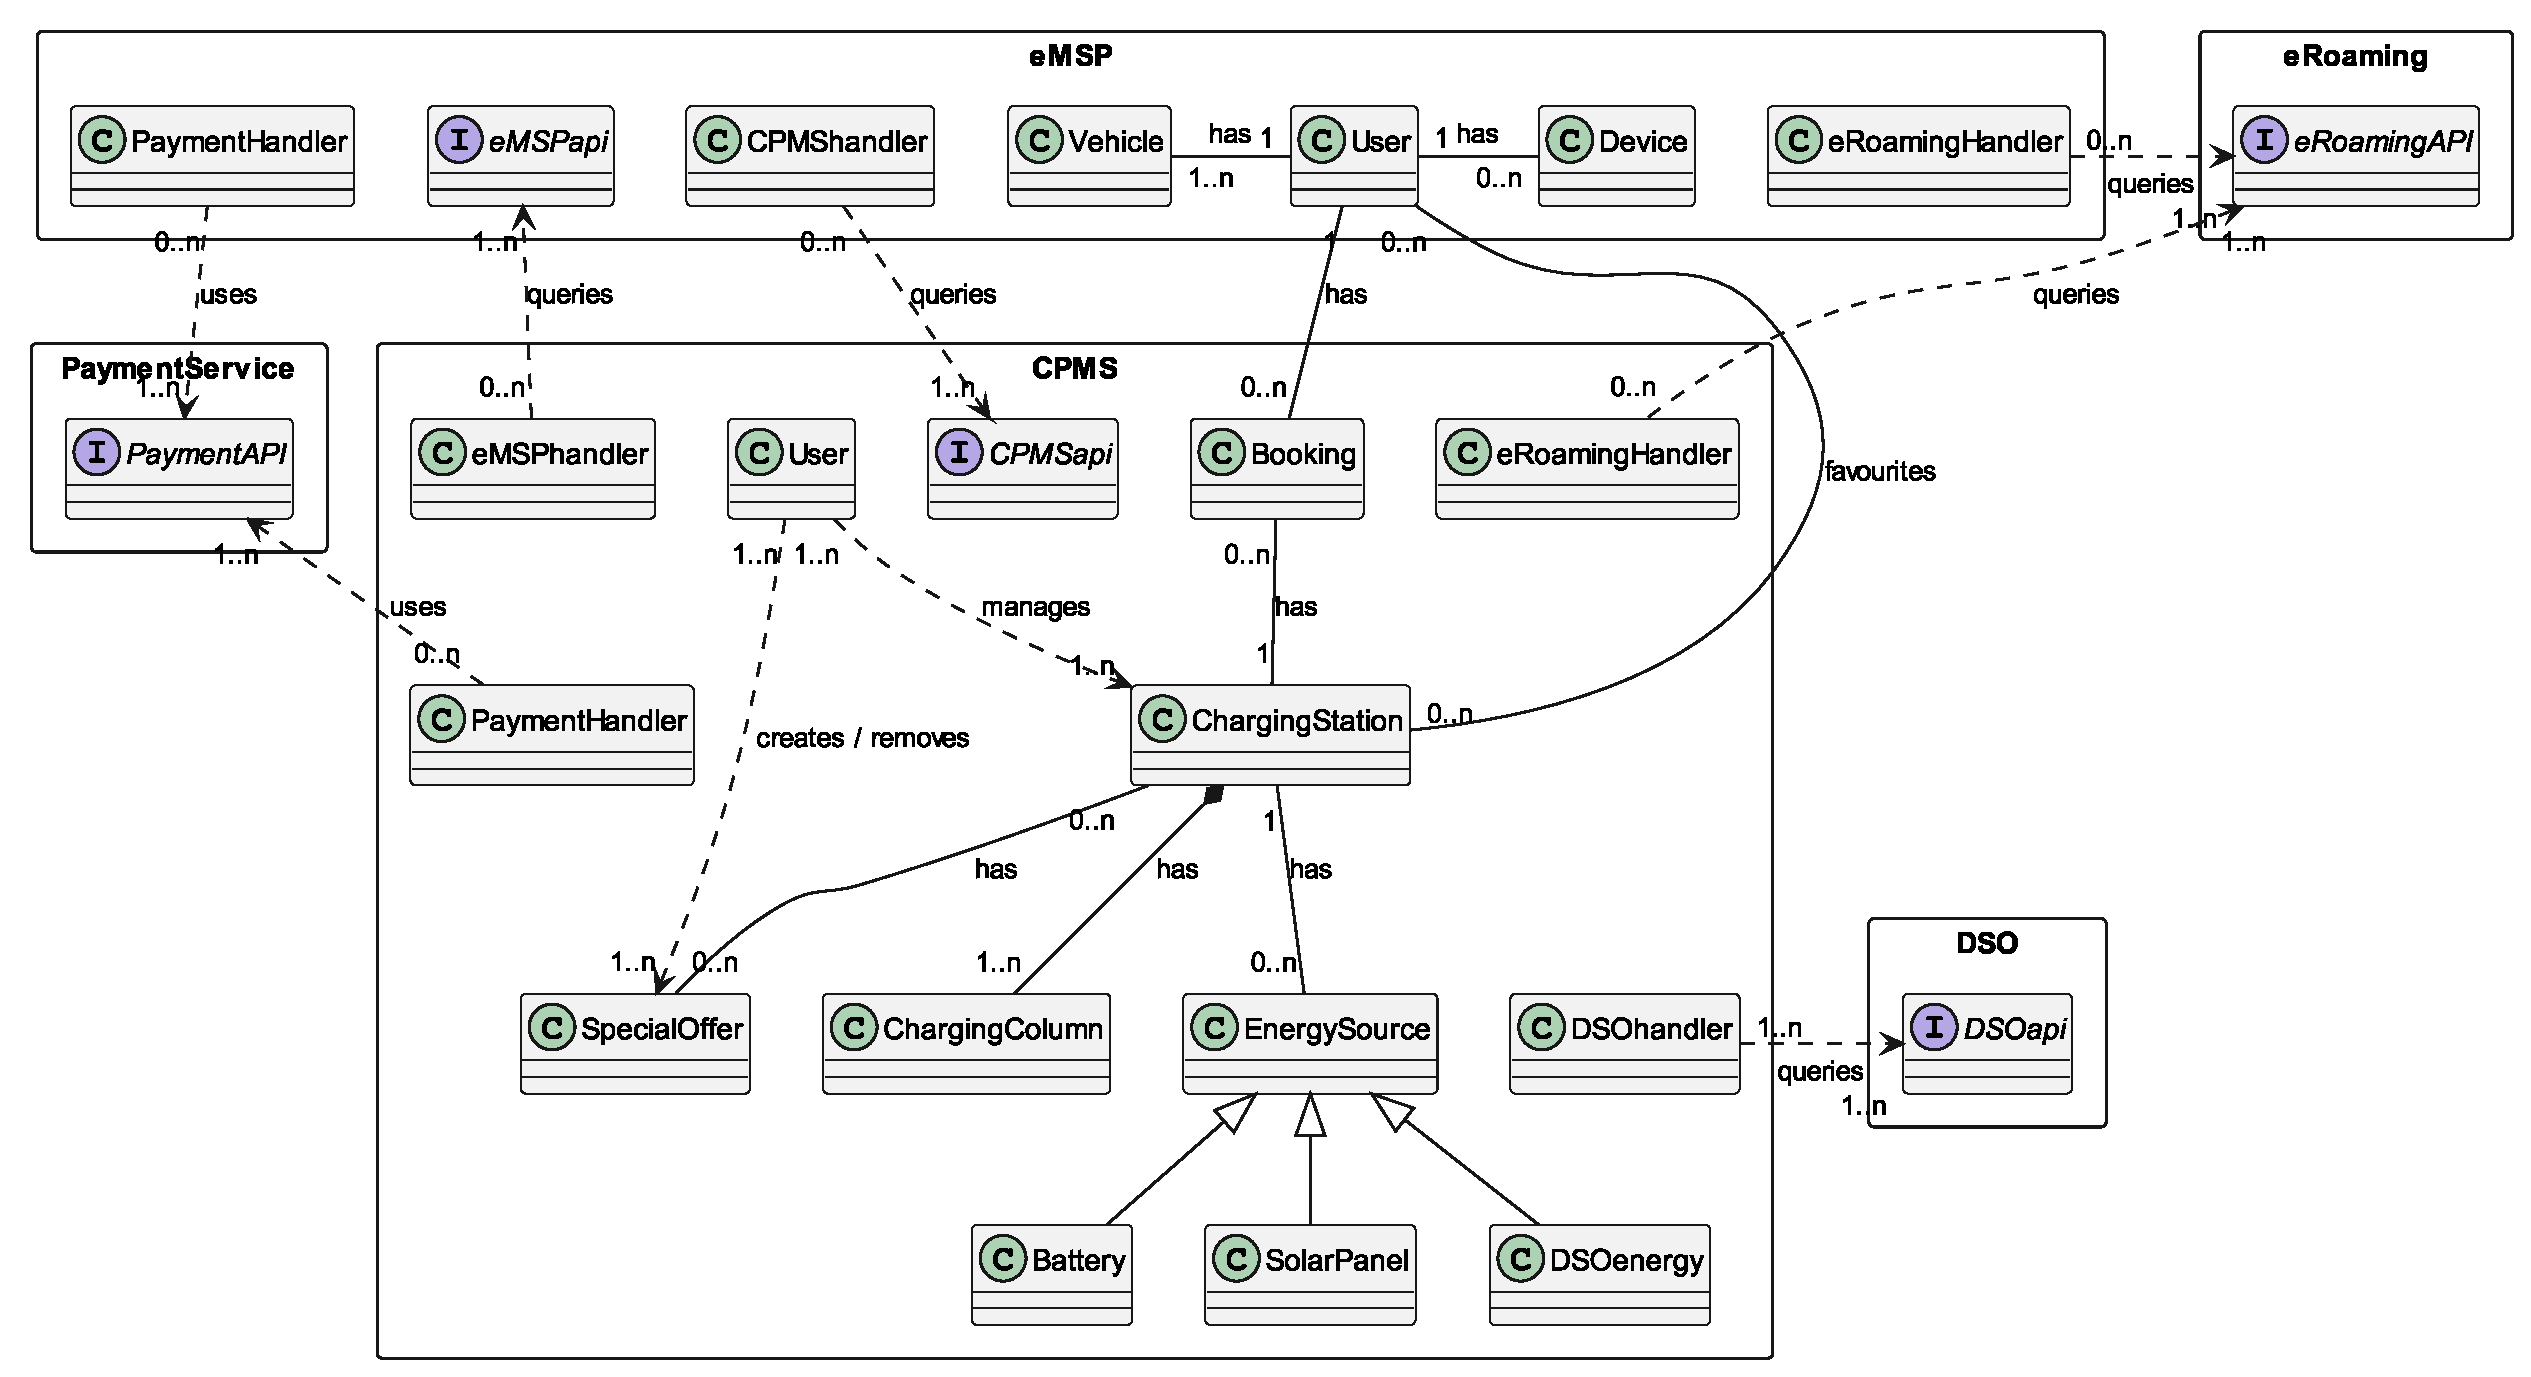
\includegraphics[width=0.99\columnwidth]{./images/diagrams/class}
    \caption{the class diagram of the various systems with the main interactions.}
\end{figure}

\pagebreak

\section{eMSP functions}

This section explains all the different functionalities that the eMSP provides to the end users (consumers).

\paragraph{Note} All the notifications that are mentioned in this section are in-app notifications (or emails, if the user selected this as the preferred notification method) that can be sent to the user only if there is at least one user's logged-in device with his/her credentials, otherwise, the email is chosen for the notification. If the notification derives from direct user interactions within the application, in-app notifications are sent only to the logged-in devices of the user which aren't the ones s/he has used to perform that action.

\subsection{Registration and login/logout}

Every new user who wants to register is asked to provide some basic information, like name, surname, birthdate, an email address that will be used as the username, and a password (which has to be given twice).\medskip

In case the email address is already present in the database or the two password fields don't coincide, the sign-up request is aborted, and the user is notified about this. If otherwise, the request ends successfully, the user receives an email at the specified address (username) with a confirmation link that expires within 24h from the emission. If the user doesn't confirm the address, the registration is automatically deleted. When the account is confirmed it becomes accessible through the login procedure and a confirmation email is sent to the user.\medskip

Every registered user can log into the system by providing username and password. If both are present in the database and the account has been confirmed, the user is granted access to his/her private area in which s/he can look for a charging station, book a charge or pay for it (and a few more other functionalities). Moreover, there is the possibility to log out. This deletes all the information stored locally on the user's device preventing him/her from accessing the account before logging in again.

\subsection{Look for nearby stations}

Every logged user can access a page with all the charging stations which can be sorted by distance (manually inserting the location or geolocalizing the user's device), by price (taking into account also any eventual discounts), or by availability. The user is also given the possibility to select a charging station, in which case the system will provide all the information related to that station, like the name, the precise location (address), the price for the charge, the number of parking slots for recharging and a calendar with all the availabilities (the available slots per period of time). Moreover, here is where the user is given the possibility to book a charge (which is described below in the next subsection).

\subsection{Book a charging station for a certain timeframe}

The booking of a charging slot is to be intended as the prosecution of the preceding subsection.\medskip

When the user wants to book a slot in a specific station, s/he selects the car s/he wants to charge (if more than one is associated), and the system gives him/her all the available consecutive time slots\footnote{Available consecutive time slots are adjacent time slots at a specific charging column. As an example, if there are only two available adjacent time slots related to two different charging columns at the same station, they aren't shown as a unique slot since the user would be forced to move the vehicle in the middle of the charge between the two columns.} for every day (with a fixed maximum look ahead from the current date). The system will try, as much as possible, to organize the physical slots according to the reservations, so it gives the user only an aggregated view of the availabilities. In any case, if the reservation ends successfully, the system sends a notification with the details of the reservation and the possibility to add it to the calendar.

\subsection{Receive important notifications}

15 minutes before the booked charge (or immediately if the user books a charge for that moment), the user receives a notification indicating the exact charging slot s/he has been assigned by the system for the charge.\medskip

Moreover, once the CPMS notices that the charging process of the user's vehicle is finished\footnote{This, of course, works only if the user booked that charging slot, otherwise, the system is structured in a way that it forbids the user to recharge the vehicle by simply not charging it.}, it informs the eMSP which sends a notification to the user, telling that the charge is finished, and that s/he can proceed in removing the socket and the vehicle from the charging zone and paying for the service.

\vfill

\subsection{Pay for the service}

After the charge is finished, the user is allowed to pay for the obtained service. This can be done through an apposite section in his/her personal area in the application or through a physical in-place device\footnote{The physical in-place device can be a POS (like pretty much on every vending machine at Politecnico di Milano) or another kind of device that allows payments.}. In any case, the user is notified once the payment is completed (both in case of success and failure). If the payment fails, the user can retry it, and this process repeats until the user successfully pays for the service.

\subsection{Query external services}

The system periodically queries an eRoaming service that informs it about all the available CPOs that subscribed to that network. From that moment on, the eMSP can interact with all their specific CPMSs, exchanging information thanks to the use of standard APIs.

\section{CPMS functions}

This section, instead, covers all the functionalities that the CPMS should provide to the authorized users of the CPO.

\subsection{Login/logout}

Every registered user can log into the system by providing a username and password. If a match is found in the database, the user is granted access to the area where s/he can manage the allowed charging station. Having logged in, the user can at any point log out from the website.

\subsection{Manage energy mix}

After login, users can define a new energy mix to be used by the system for a specific charge station. This includes defining from which sources energy is provided to sockets and if batteries are to be recharged, used, or ignored. Users can also let the system automatically define energy mixes that can change over time.

\subsection{Manage DSO choice}

After login, users can select what DSO is being used by the system, or let the system choose automatically based on the lowest rates. DSO rates can be queried from a list of available DSOs.

\subsection{Get info about a charging station's internal/external status}

After login, users can query information about a charging station's external status. This includes all available charging columns and relative sockets and how many cars are present. Users can also query information about a charging station's internal status. This includes amounts of energy available in its batteries, and for each charging vehicle, the amount of power absorbed and time left to the end of the charge.

\subsection{Manage special offers}

After login, users can create a new special offer by specifying a start date, an end date, and a discount amount. Special offers can be expanded in future versions of the system. Users can also delete an existing special offer, to make up for mistakes in the making of a new special offer.

\vfill
\pagebreak

\section{User characteristics} \label{users}

In this section are described all the various classes of users who are interacting with the system\footnote{For the sake of simplicity, the obvious superusers (the administrators) of each system are not presented here.}.

\subsection{Consumer (end user)}

The consumer is the end user of the eMSP system: s/he's the one that wants to charge an electric vehicle. The consumer can look for a charging station thanks to the use of a map integrated into the mobile application, and when s/he identifies a satisfying one (s/he can look for availability, price\dots), s/he can book a charge in a specific time slot at that station (if there is still any available). Once the charge is finished, s/he receives a notification from the application on the smartphone or, if preferred, an email. When s/he takes away the vehicle after the charge, s/he can pay for the obtained service, directly at the charging station or through an apposite function on the application.

\subsection{CPO's authorized user}

The CPO's authorized user is the end user of the CPMS system. S/he owns charging stations and can manage the charging columns via the CPMS. S/he can make decisions regarding which DSO to acquire energy from, change the cost of charges, set special offers, and decide how to direct the flow of energy in presence of multiple sources (for example if solar panels or batteries are available). S/he can also monitor the external and internal situation of charging stations, as to infer information about bottlenecks in the management of the system (for example if a station is always crowded it would be wise to consider expanding it with new charging columns) and information regarding the health of components (like in the case of local batteries).

\section{Domain assumptions}

These are all the domain assumptions done in order to write the specifications of this system.

\begin{center}
    \begin{tabular}{ | >{\centering\arraybackslash}m{0.1\columnwidth} | >{\arraybackslash}m{0.84\columnwidth} | }
        \hline
        \textbf{Identifier} & \multicolumn{1}{c|}{\textbf{Description}} \\
        \hline
        \hline
        \showD{d:connect} & Users can connect to the internet and access the service. \\
        \hline
        \showD{d:plug} & Consumers know how to manage the vehicle charging process, plugging and unplugging the vehicle. \\
        \hline
        \showD{d:remove} & Consumers remove their vehicles by the end of the booked charging slot. \\
        \hline
        \showD{d:truth} & Consumers provide true and correct information when registering on the platform. \\
        \hline
        \showD{d:vehicle} & Every vehicle that uses the system has a certificate used for authenticating it at the charging column and the consumer can access it. \\
        \hline
        \showD{d:dso} & DSOs provide true and correct data to CPOs. \\
        \hline
        \showD{d:abusive} & No one abusively parks in the slots. \\
        \hline
        \showD{d:harm} & No physical harm is done to the equipment at the charging stations. \\
        \hline
        \showD{d:unauthorized} & No unauthorized person can alter the state of the charging station (plugging and unplugging cables, opening the stations\dots). \\
        \hline
        \showD{d:batteries} & Batteries are durable/stable during the charging process (both in cars and charging stations). \\
        \hline
        \showD{d:dso_energy} & Charging stations are designed to not have energy shortages, even in case of full load. \\
        \hline
        \showD{d:socket} & All sockets types are compatible, but charge speed is not guaranteed for different types. \\
        \hline
        \showD{d:charge} & Sooner or later the charging process of every vehicle ends (the vehicle is fully charged, or the time slot is ended). \\
        \hline
        \showD{d:reliable} & There is a reliable network and structure to connect all the components outside the managed infrastructure. \\
        \hline
        \showD{d:payment} & All payments are handled by a third party and go through correctly (either commit or abort, notifying the result to both the user and the system). \\
        \hline
        \showD{d:api} & Uniform APIs already exist and are already implemented in the other systems in order to simplify the communication between all the different service providers. \\
        \hline
        \showD{d:cpo} & Only users authorized by CPOs can be given credentials to access the CPMS and manage it. \\
        \hline
        \showD{d:eroaming} & There exists an eRoaming service, already configured on the systems, that allows them to discover each other. \\
        \hline
    \end{tabular}
\end{center}

    \chapter{Specific Requirements} \label{requirements}

\section{External interface requirements}

\subsection{User interfaces}

\paragraph{eMSP} The system should be available to the end users in form of a web page and an accessible mobile application (which will be able to receive in-app notifications). In both cases, the user has to be connected to the internet.

\paragraph{CPMS} The system should be available to the end users in form of a web page. The ease of use is not of the outermost importance, and it's not to be preferred over a more complete and condensed view. Priority should be given to offering all functionalities in the quickest possible way and showing relevant information in the clearest way. Users are required to know how to use the system to fully be able to operate all functionalities (this can be done through the design of a user manual).

\subsection{Hardware interfaces}

\paragraph{eMSP} The eMSP doesn't have any particular hardware constraint, but its frontends should be run on any mobile device and computer (in this case only through a browser). Its backend only needs servers able to respond to the user's queries.

\paragraph{CPMS} The only hardware interface needed to access the CPMS is a computer with an installed browser since all functionalities are being offered through a website.

\subsection{Software interfaces}

\paragraph{APIs} The communication between the different systems should happen thanks to the use of standard APIs. All the systems described in this document should be also able to communicate with external systems which expose the same APIs.

\paragraph{eRoaming} There exists an eRoaming service that is accessible thanks to an API that allows eMSPs to query about available CPOs and their location. It also provides the eMSP with the endpoint address of every selected CPMS (CPO's backend).

\paragraph{OpenStreetMap} The eMSP application uses the OpenStreetMap API to provide the map of all the connected charging stations of the various CPOs.

\section{Functional requirements}

\subsection{Requirements}

\paragraph{eMSP requirements}

\begin{center}
    \begin{tabular}{ | >{\centering\arraybackslash}m{0.1\columnwidth} | >{\arraybackslash}m{0.84\columnwidth} | }
        \hline
        \textbf{Identifier} & \multicolumn{1}{c|}{\textbf{Description}} \\
        \hline
        \hline
        \showR{r:e:signup} & The system must allow the user to sign-up. \\
        \hline
        \showR{r:e:signup_check} & The system must check the sign-up data. \\
        \hline
    \end{tabular}
\end{center}
\begin{center}
    \begin{tabular}{ | >{\centering\arraybackslash}m{0.1\columnwidth} | >{\arraybackslash}m{0.84\columnwidth} | }
        \hline
        \textbf{Identifier} & \multicolumn{1}{c|}{\textbf{Description}} \\
        \hline
        \hline
        \showR{r:e:signup_mail} & The system must send the user an email for activating the account after a successful sign-up. \\
        \hline
        \showR{r:e:signup_activation} & The system must discard any account activation request that arrives after 24 hours from the sign-up procedure. \\
        \hline
        \showR{r:e:signup_not_activated} & The system must consider any signed-up user who hasn't already activated the account as an unregistered user. \\
        \hline
        \showR{r:e:signup_success} & The system must notify the user of the sign-up result, sending an email if it's successful. \\
        \hline
        \showR{r:e:login} & The system must allow the user to log in. \\
        \hline
        \showR{r:e:login_check} & The system must check the login data. \\
        \hline
        \showR{r:e:pwchange} & The system must allow the user to change his/her password after logging in. \\
        \hline
        \showR{r:e:pwreset} & The system must allow any registered user to reset his/her password by sending an email to the specified address. \\
        \hline
        \showR{r:e:pwreset_timeout} & The system must discard any password change 24 hours after the request. \\
        \hline
        \showR{r:e:pwreset_duplicate} & The system must discard any duplicated usage of the same link for password change after a successful one. \\
        \hline
        \showR{r:e:logout} & The system must allow the user to logout. \\
        \hline
        \showR{r:e:notification} & The system must allow the user to set the preferred notification method. \\
        \hline
        \showR{r:e:car_add} & The system must allow the user to add a new vehicle. \\
        \hline
        \showR{r:e:car_remove} & The system must allow the user to remove an associated vehicle, only if there is at least one. \\
        \hline
        \showR{r:e:car_edit} & The system must allow the user to edit any associated vehicle's details. \\
        \hline
        \showR{r:e:stations_lookup} & The system must allow the user to look for nearby stations. \\
        \hline
        \showR{r:e:stations_sort} & The system must allow the user to sort the nearby stations according to distance, price, and availability. \\
        \hline
        \showR{r:e:stations_favorite_mark} & The system must allow the user to mark and unmark stations as \doublequotes{favorite}. \\
        \hline
        \showR{r:e:book} & The system must allow the user to book a charge in a charging station if any slot is available. \\
        \hline
        \showR{r:e:book_car} & The system must ask the user the vehicle s/he wants to charge every time s/he books a charge. \\
        \hline
        \showR{r:e:book_notification} & The system must notify the user of any successful booked charge. \\
        \hline
        \showR{r:e:book_add_calendar} & The system must allow the user to add any booked charge to the calendar. \\
        \hline
        \showR{r:e:book_all} & The system must allow the user to show all the booked charges, both past, and future (there might be limits). \\
        \hline
        \showR{r:e:book_edit} & The system must allow the user to edit or delete a booked charge before the end of the booked slot. \\
        \hline
        \showR{r:e:book_notification_slot} & The system must notify the user of the charging slot to use before the charge. \\
        \hline
        \showR{r:e:book_notification_end} & The system must notify the user when the charge is finished. \\
        \hline
        \showR{r:e:payment} & The system must allow the user to pay for the obtained service. \\
        \hline
        \showR{r:e:payment_notification} & The system must notify the user after every payment attempt (both in case of success and failure). \\
        \hline
        \showR{r:e:eroaming} & The system must periodically contact an eRoaming service for obtaining the list of available CPOs (and respective CPMSs). \\
        \hline
        \showR{r:e:cpms_connect} & The system must be able to connect to any CPMS that offers standard APIs. \\
        \hline
        \showR{r:e:cpms_communicate} & The system must be able to communicate with any connected CPMS through standard APIs. \\
        \hline
        \showR{r:e:user_registered} & The system must allow any registered user to do everything specified, except signing up. \\
        \hline
        \showR{r:e:user_unregistered} & The system must allow any unregistered user to only sign up and log in. \\
        \hline
        \showR{r:e:notification_app} & The system must send the notification only to the user's authenticated devices if the notification preference is by in-app notification. \\
        \hline
        \showR{r:e:notification_mail} & The system must send emails instead of in-app notifications if that's the user's preferred method or if there is no available user's device. \\
        \hline
    \end{tabular}
\end{center}

\pagebreak

\paragraph{CPMS requirements}

\begin{center}
    \begin{tabular}{ | >{\centering\arraybackslash}m{0.1\columnwidth} | >{\arraybackslash}m{0.84\columnwidth} | }
        \hline
        \textbf{Identifier} & \multicolumn{1}{c|}{\textbf{Description}} \\
        \hline
        \hline
        \showR{r:c:input} & The system must check all input data correctness. \\
        \hline
        \showR{r:c:login} & The system must allow the user to log in. \\
        \hline
        \showR{r:c:pwchange} & The system must allow the user to change his/her password after logging in. \\
        \hline
        \showR{r:c:pwreset} & The system must allow any registered user to reset his/her password by sending an email to the specified address. \\
        \hline
        \showR{r:c:pwreset_timeout} & The system must discard any password change 24 hours after the request. \\
        \hline
        \showR{r:c:pwreset_duplicate} & The system must discard any duplicated usage of the same link for password change after a successful one. \\
        \hline
        \showR{r:c:logout} & The system must allow the user to logout. \\
        \hline
        \showR{r:c:API_show_booking} & The system must provide an API function to get information about all bookings present for any charging station. \\
        \hline
        \showR{r:c:API_book} & The system must provide an API function to add/delete a booking for a charging point in a charging station. \\
        \hline
        \showR{r:c:API_stations} & The system must provide an API function to get information about all charging points and respective sockets in a charging station. \\
        \hline
        \showR{r:c:API_prices} & The system must provide an API function to get information about prices relative to a charging station and socket types. \\
        \hline
        \showR{r:c:start_car_charge} & The system must start charging a car when it is first plugged in if it corresponds to the car for which a charge was booked in the corresponding time and place (same charging point/socket as well). \\
        \hline
        \showR{r:c:stop_car_charge_full} & The system must stop charging a car once it recognizes that the car battery has reached full capacity. \\
        \hline
        \showR{r:c:stop_car_charge_time} & The system must stop charging a car if the booking corresponding to that car ends and the car is still plugged in. \\
        \hline
        \showR{r:c:autoselect_DSO} & The system must automatically select the DSO that offers the best energy price if the “automatic DSO choice” is selected. \\
        \hline
        \showR{r:c:stop_battery_charge_full} & If a battery was charging and reaches a full charge, the system must stop charging the battery. \\
        \hline
        \showR{r:c:auto_mix} & The system must automatically change the energy mix if the \doublequotes{automatic mix choice} is selected. \\
        \hline
        \showR{r:c:notification_column} & The system must automatically notify the eMSP of the assignment of a charging column. \\
        \hline
        \showR{r:c:notification_charge} & The system must automatically notify the eMSP of the end of the car charge. \\
        \hline
        \showR{r:c:periodical_updates} & The system must periodically update the database with new data coming from sensors present in charging stations. \\
        \hline
        \showR{r:c:view_bookings} & The system must allow the CPMS user to view all bookings present for any charging station. \\
        \hline
        \showR{r:c:view_charging_point} & The system must allow the CPMS user to view all charging points, relative socket types, and if they are occupied or not, for any charging station. \\
        \hline
        \showR{r:c:view_battery_levels} & The system must allow the CPMS user to view the batteries' charge levels if present. \\
        \hline
        \showR{r:c:manage_offers} & The system must allow the CPMS user to create and delete special charge offers. \\
        \hline
        \showR{r:c:view_DSO} & The system must allow the CPMS user to view all DSO available. \\
        \hline
        \showR{r:c:view_DSO_prices} & The system must allow the CPMS user to view all DSO prices. \\
        \hline
        \showR{r:c:change_mix} & The system must allow the CPMS user to change the energy mix. \\
        \hline
        \showR{r:c:start_battery_charge} & The system must allow the CPMS user to start recharging batteries if they are present. \\
        \hline
        \showR{r:c:auto_DSO} & The system must allow the CPMS user to activate and deactivate \doublequotes{automatic DSO choice}. \\
        \hline
        \showR{r:c:auto_MIX} & The system must allow the CPMS user to activate and deactivate \doublequotes{automatic mix choice}. \\
        \hline
        \showR{r:c:DSO_payment} & The system must allow the CPMS user to modify the automatic DSO payment method. \\
    \hline
    \end{tabular}
\end{center}

\pagebreak

\subsection{Goal mapping}

\paragraph{eMSP goals}

\begin{center}
    \begin{tabular}{ | >{\centering\arraybackslash\bfseries}m{0.06\columnwidth} | >{\arraybackslash}m{0.36\columnwidth} | >{\arraybackslash}m{0.5\columnwidth} | }
        \hline
        Goal & \multicolumn{1}{c|}{\textbf{Domain assumptions}} & \multicolumn{1}{c|}{\textbf{Requirements}} \\
        \hline
        \hline
        \refG{g:e:lookup} & \refD{d:connect}, \refD{d:truth}, \refD{d:reliable}, \refD{d:api}, \refD{d:eroaming} & \refR{r:e:signup}-\refR{r:e:notification}, \refR{r:e:stations_lookup}, \refR{r:e:stations_sort}, \refR{r:e:stations_favorite_mark}, \refR{r:e:eroaming}, \refR{r:e:cpms_connect}, \refR{r:e:cpms_communicate}, \refR{r:e:user_registered}, \refR{r:e:user_unregistered} \\
        \hline
        \refG{g:e:book} & \refD{d:connect}, \refD{d:truth}, \refD{d:vehicle}, \refD{d:reliable}, \refD{d:api} & \refR{r:e:signup}-\refR{r:e:notification}, \refR{r:e:car_add}-\refR{r:e:car_edit}, \refR{r:e:book}-\refR{r:e:book_notification_slot}, \refR{r:e:cpms_communicate}, \refR{r:e:user_registered}-\refR{r:e:notification_mail} \\
        \hline
        \refG{g:e:start} & \refD{d:plug}-\refD{d:vehicle}, \refD{d:abusive}-\refD{d:unauthorized}, \refD{d:dso_energy}, \refD{d:socket}, \refD{d:reliable}, \refD{d:api} & \refR{r:e:car_add}-\refR{r:e:car_edit}, \refR{r:e:cpms_communicate}, \refR{r:e:user_registered}, \refR{r:e:user_unregistered} \\
        \hline
        \refG{g:e:notify} & \refD{d:connect}, \refD{d:truth}, \refD{d:charge}, \refD{d:reliable}, \refD{d:api} & \refR{r:e:signup}-\refR{r:e:notification}, \refR{r:e:car_add}-\refR{r:e:car_edit}, \refR{r:e:book_notification_end}, \refR{r:e:cpms_communicate}, \refR{r:e:user_registered}-\refR{r:e:notification_mail}, \refR{r:c:notification_column}, \refR{r:c:notification_charge} \\
        \hline
        \refG{g:e:pay} & \refD{d:connect}, \refD{d:truth}, \refD{d:harm}, \refD{d:charge}-\refD{d:api} & \refR{r:e:signup}-\refR{r:e:notification}, \refR{r:e:car_add}-\refR{r:e:car_edit}, \refR{r:e:payment}, \refR{r:e:payment_notification}, \refR{r:e:user_registered}-\refR{r:e:notification_mail} \\
        \hline
    \end{tabular}
\end{center}

\paragraph{CPMS goals}

\begin{center}
    \begin{tabular}{ | >{\centering\arraybackslash\bfseries}m{0.06\columnwidth} | >{\arraybackslash}m{0.36\columnwidth} | >{\arraybackslash}m{0.5\columnwidth} | }
        \hline
        Goal & \multicolumn{1}{c|}{\textbf{Domain assumptions}} & \multicolumn{1}{c|}{\textbf{Requirements}} \\
        \hline
        \hline
        \refG{g:c:info} & \refD{d:vehicle}, \refD{d:abusive}, \refD{d:harm}, \refD{d:batteries}, \refD{d:charge}, \refD{d:reliable} & \refR{r:e:book}, \refR{r:e:book_all}, \refR{r:e:book_edit}, \refR{r:e:book_notification_slot}, \refR{r:c:API_show_booking}-\refR{r:c:API_prices}, \refR{r:c:periodical_updates}, \refR{r:c:view_bookings}-\refR{r:c:view_battery_levels} \\
        \hline
        \refG{g:c:charge} & \refD{d:vehicle}, \refD{d:abusive}-\refD{d:unauthorized}, \refD{d:dso_energy}-\refD{d:reliable}, \refD{d:api}, \refD{d:cpo} & \refR{r:c:API_show_booking}, \refR{r:c:start_car_charge}-\refR{r:c:stop_car_charge_time}, \refR{r:c:notification_column}, \refR{r:c:notification_charge} \\
        \hline
        \refG{g:c:dso} & \refD{d:connect}, \refD{d:dso}, \refD{d:reliable}, \refD{d:api}, \refD{d:cpo} & \refR{r:c:input}-\refR{r:c:logout}, \refR{r:c:autoselect_DSO}, \refR{r:c:view_DSO}, \refR{r:c:view_DSO_prices}, \refR{r:c:auto_DSO}, \refR{r:c:DSO_payment} \\
        \hline
        \refG{g:c:mix} & \refD{d:connect}, \refD{d:dso}, \refD{d:batteries}, \refD{d:dso_energy}, \refD{d:reliable}, \refD{d:api}, \refD{d:cpo} & \refR{r:c:input}-\refR{r:c:logout}, \refR{r:c:stop_battery_charge_full}, \refR{r:c:auto_mix}, \refR{r:c:change_mix}, \refR{r:c:start_battery_charge}, \refR{r:c:auto_MIX} \\
        \hline
        \refG{g:c:offers} & \refD{d:connect}, \refD{d:reliable}, \refD{d:api}, \refD{d:cpo} & \refR{r:c:input}-\refR{r:c:logout}, \refR{r:c:API_prices}, \refR{r:c:manage_offers}, \refR{r:c:view_DSO_prices} \\
        \hline
    \end{tabular}
\end{center}

\subsection{Users' use cases diagrams}

\begin{figure}[h!]
    \centering
    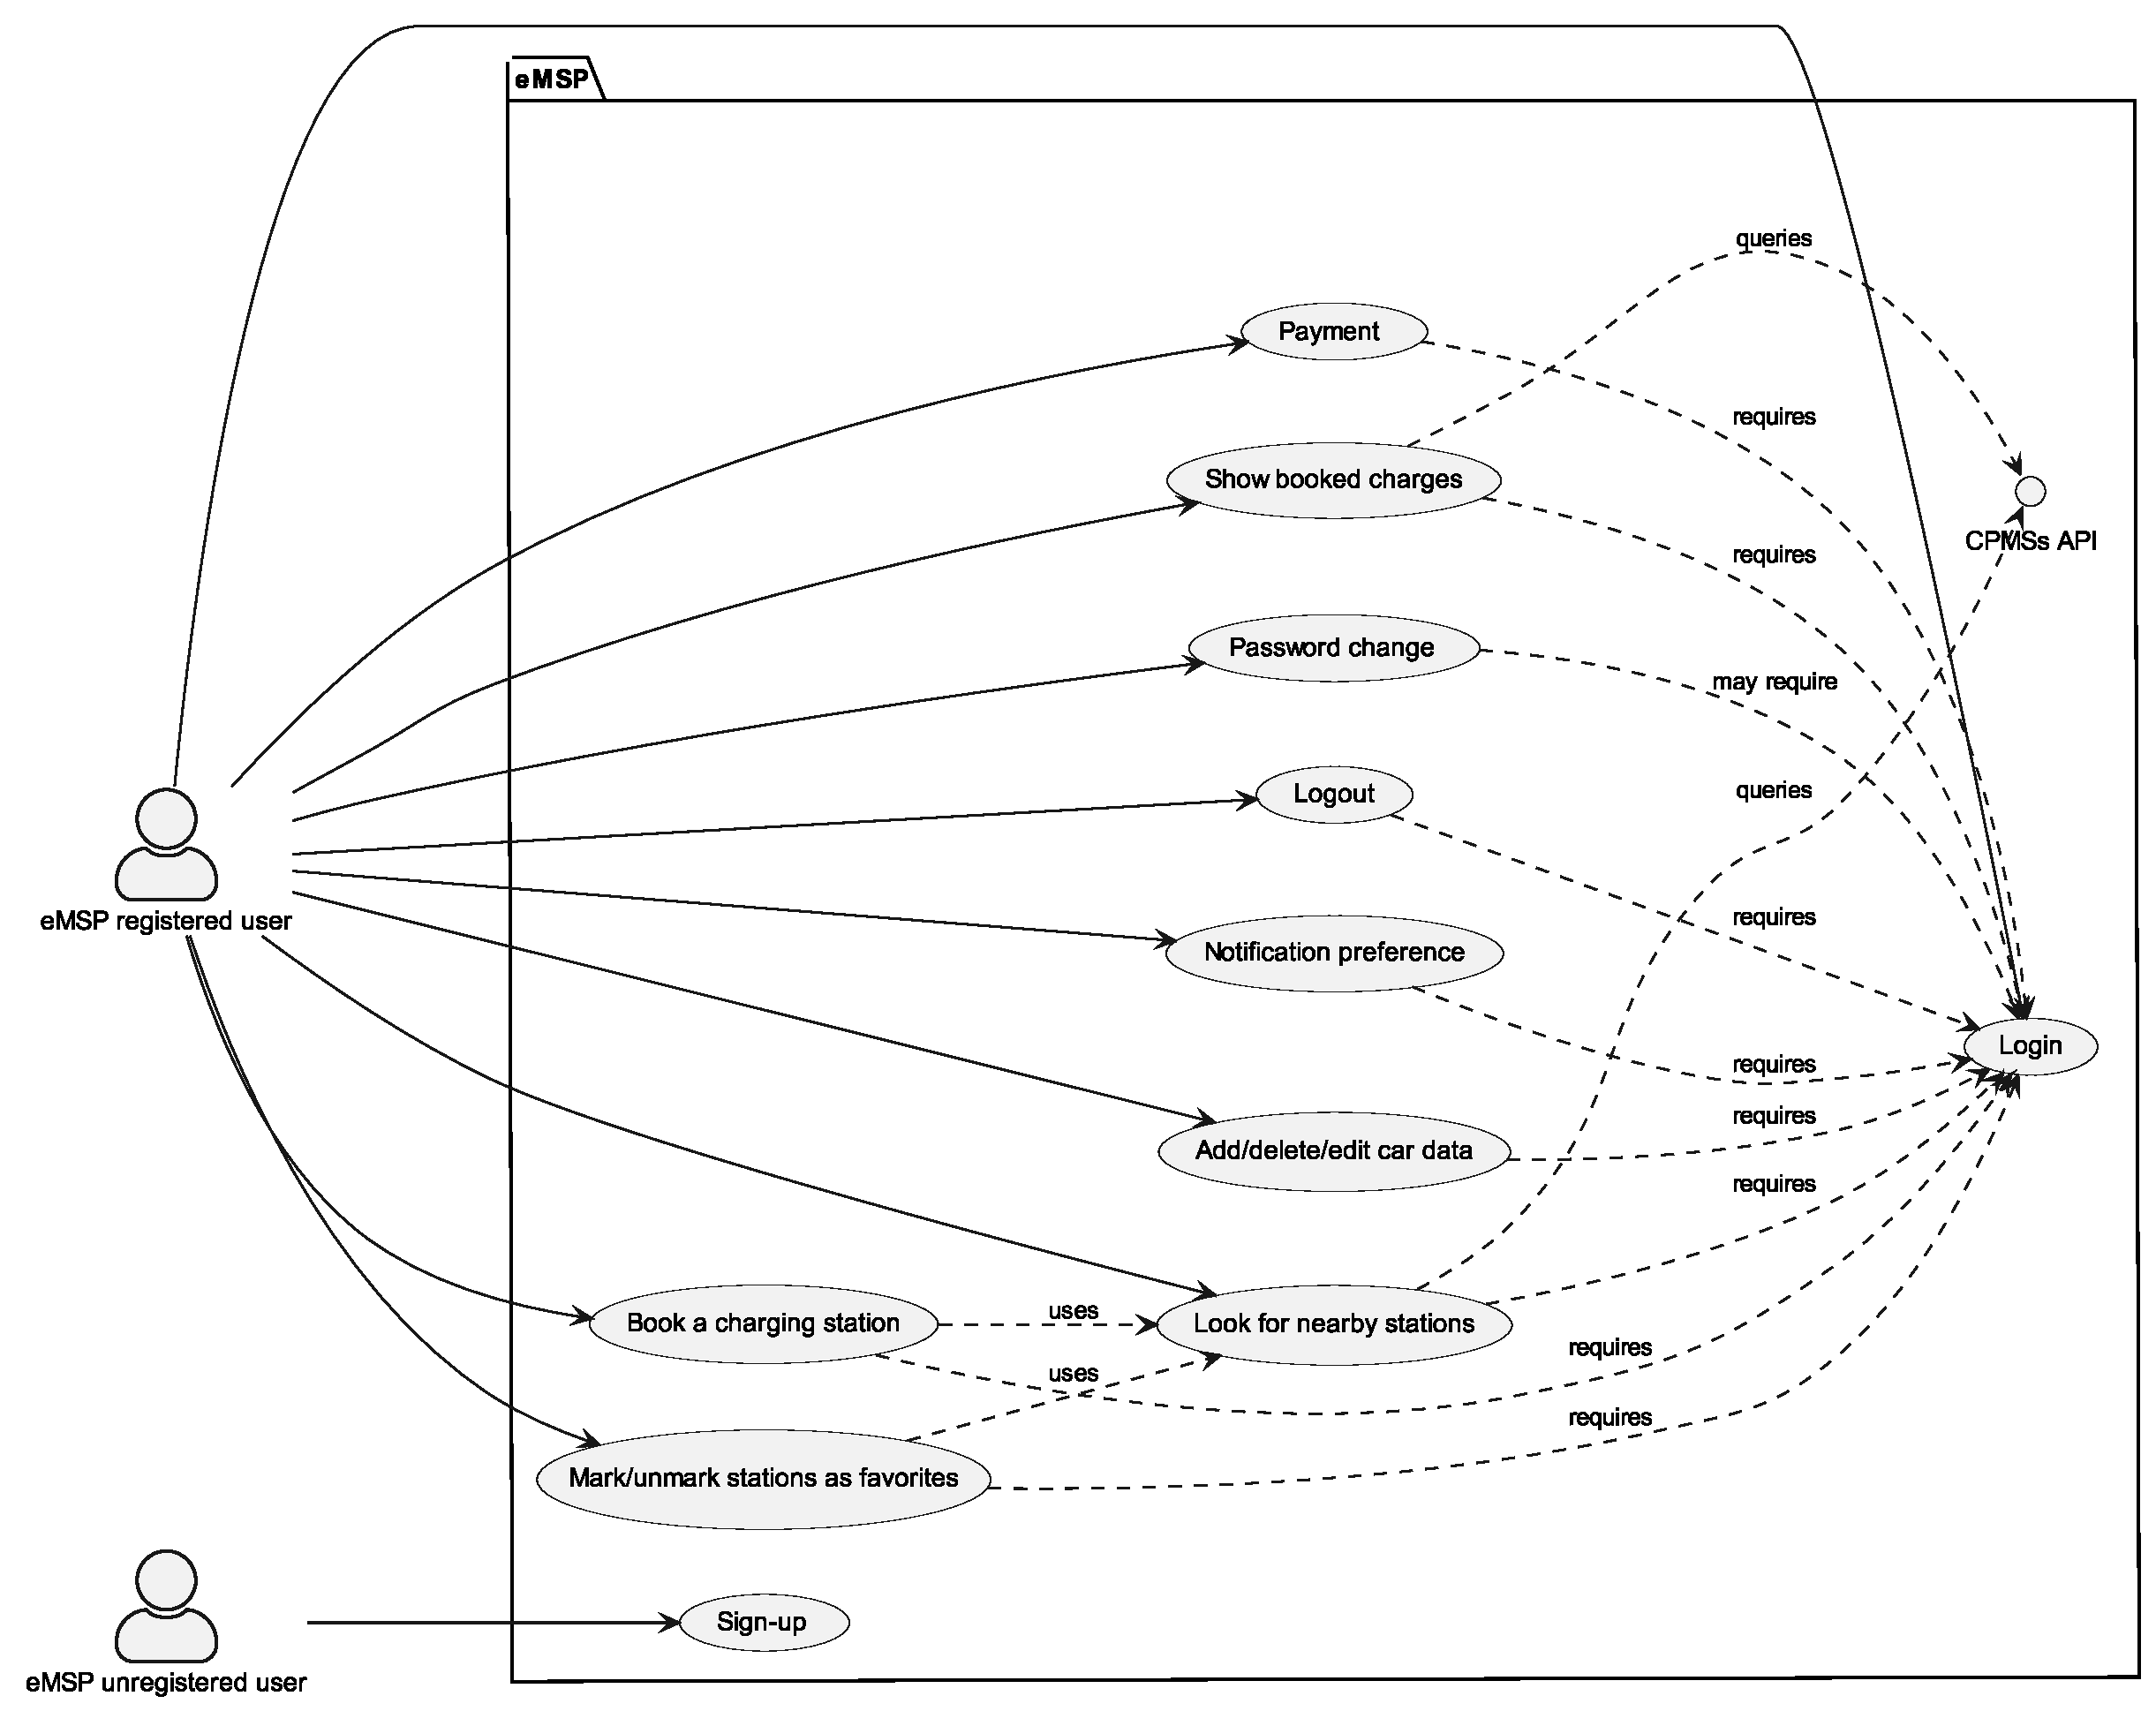
\includegraphics[width=\columnwidth]{./images/diagrams/usecases/emsp}
    \caption{eMSP users' use cases.}
\end{figure}

\begin{figure}[h!]
    \centering
    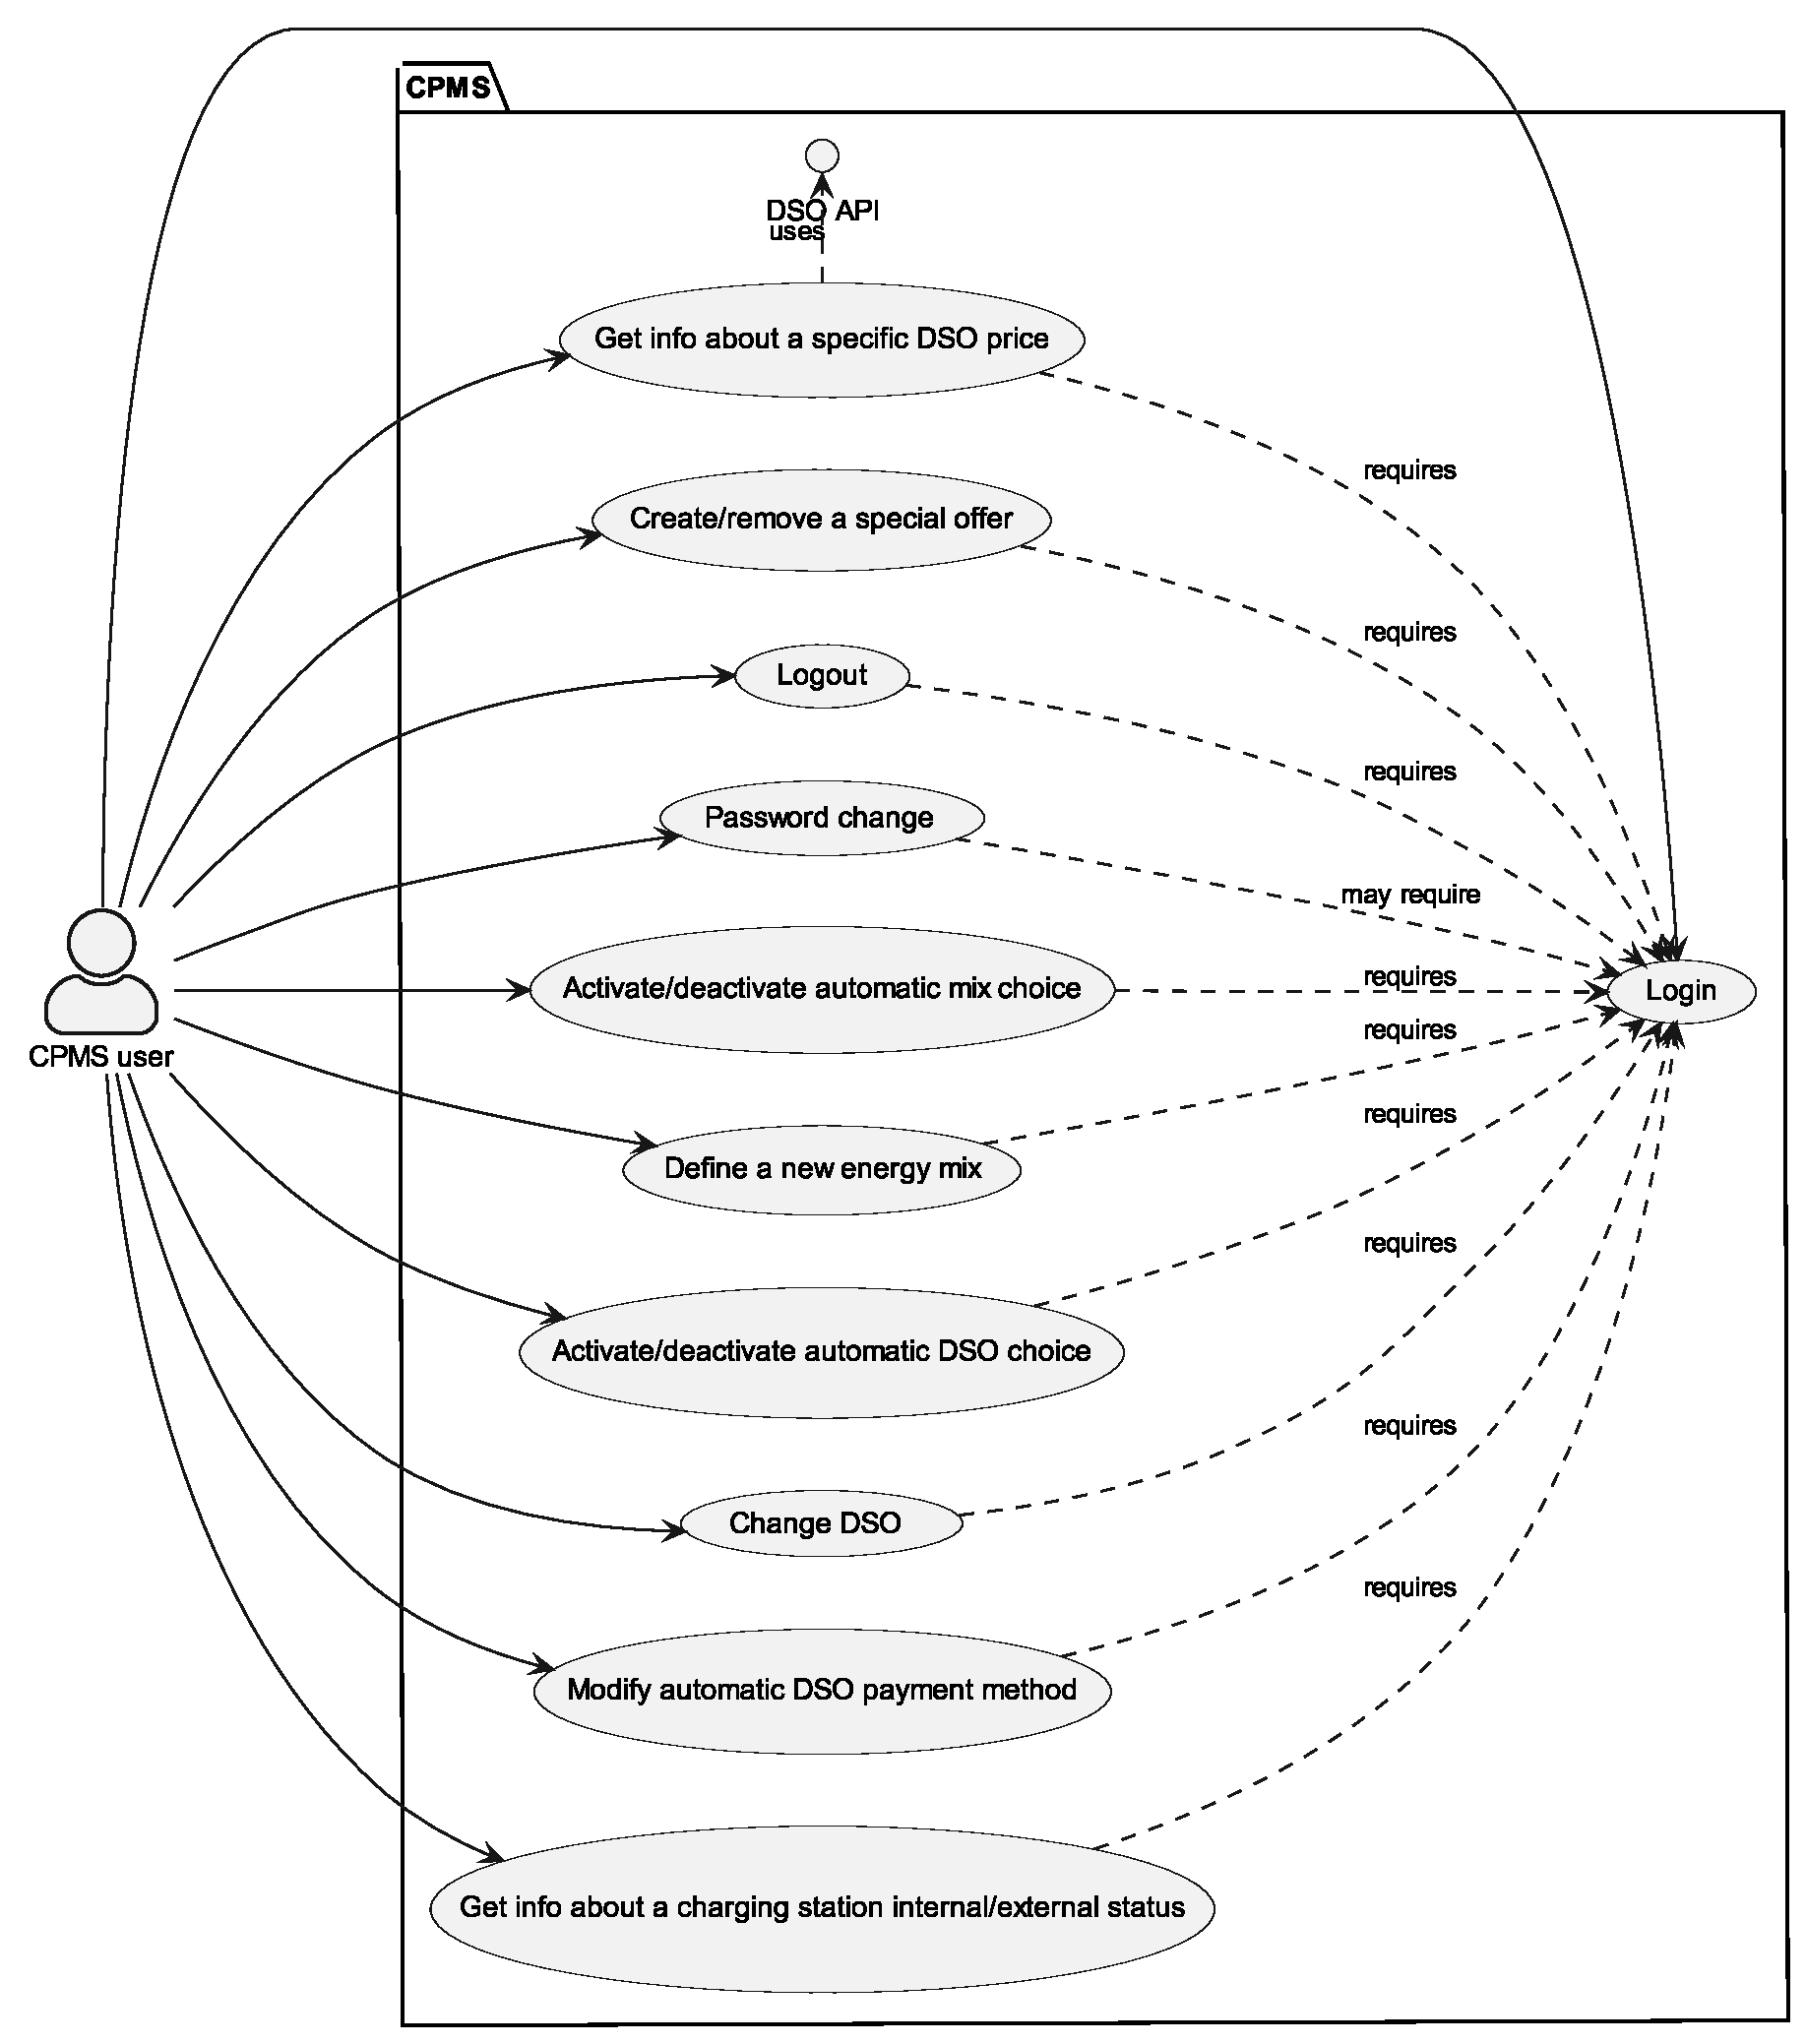
\includegraphics[width=0.8\columnwidth]{./images/diagrams/usecases/cpms}
    \caption{CPMS users' use cases.}
\end{figure}

\subsection{Use cases}

Every time \doublequotes{consumer} or \doublequotes{user} appears in a UML diagram, it's intended that s/he is interacting with the application or web page that interacts with the system.\medskip

For the sake of simplicity, many data checks and the opening of the application or web page, according to the use case, are not illustrated, but they are present in the system. Moreover, some cases are not depicted here:
\begin{itemize}
    \item \textit{Notification preference}: the user is asked to choose between in-app notifications or email ones after his first login. Furthermore, the user can change this preference at any time under his/her profile.
    \item \textit{Logout}: simply removes the token\footnote{An explanation of the usage of the token can be found in the eMSP's login use case (\refUC{uc:e:login}).} from the client.
    \item \textit{Password change}: it works like most of the password changes implemented nowadays. The first option is that the user clicks on the \doublequotes{Forgot password?} link, receives an email with the link for changing it, and changes the password. The second one is that s/he goes to the user's details page and changes the password directly from there. In both cases, s/he has to log back in on all his/her connected devices.
\end{itemize}
Also, even if it's not specified in the diagrams, if any component fails, the user is notified and the action is automatically aborted, reverting its state to the original one. The same happens in case of user's network failures (which are \doublequotes{detected}\footnote{This is a simplification, since in a distributed environment with possible byzantine failures things are a bit more complex.} through a timeout).

\vfill
\pagebreak

\paragraph{eMSP | Registration}

\begin{center}
    \begin{tabular}{ | >{\arraybackslash}m{0.17\columnwidth} | >{\arraybackslash}m{0.77\columnwidth} | }
        \hline
        \textbf{Identifier} & \showUC{uc:e:registration} \\
        \hline
        \textbf{Actor} & Consumer (end user) \\
        \hline
        \textbf{Entry condition} & The user is not already registered \\
        \hline
        \textbf{Event flow} & \medskip\parbox[b][][b]{0.76\columnwidth}{
            \begin{enumerate}[nosep, leftmargin=*]
                \item The user opens the application or webpage
                \item The user fills out the registration form
                \item The system checks the inserted data
                \item The system sends an email to the user for confirming the account
                \item The user clicks on the link for activating the account
                \item The system notifies that the account is confirmed
            \end{enumerate}
        } \\
        \hline
        \textbf{Exit condition} & The process ends without errors \\
        \hline
        \textbf{Exceptions} & \medskip\parbox[b][][b]{0.76\columnwidth}{
            \begin{itemize}[nosep, leftmargin=*]
                \item There is already a registered user with that email address
                \item The passwords don't coincide
                \item The user doesn't click on the link in the email within 24 hours
            \end{itemize}
        } \\
        \hline
        \textbf{Special requests} & The user needs to have access to an email address \\
        \hline
    \end{tabular}
\end{center}

\begin{figure}[h!]
    \centering
    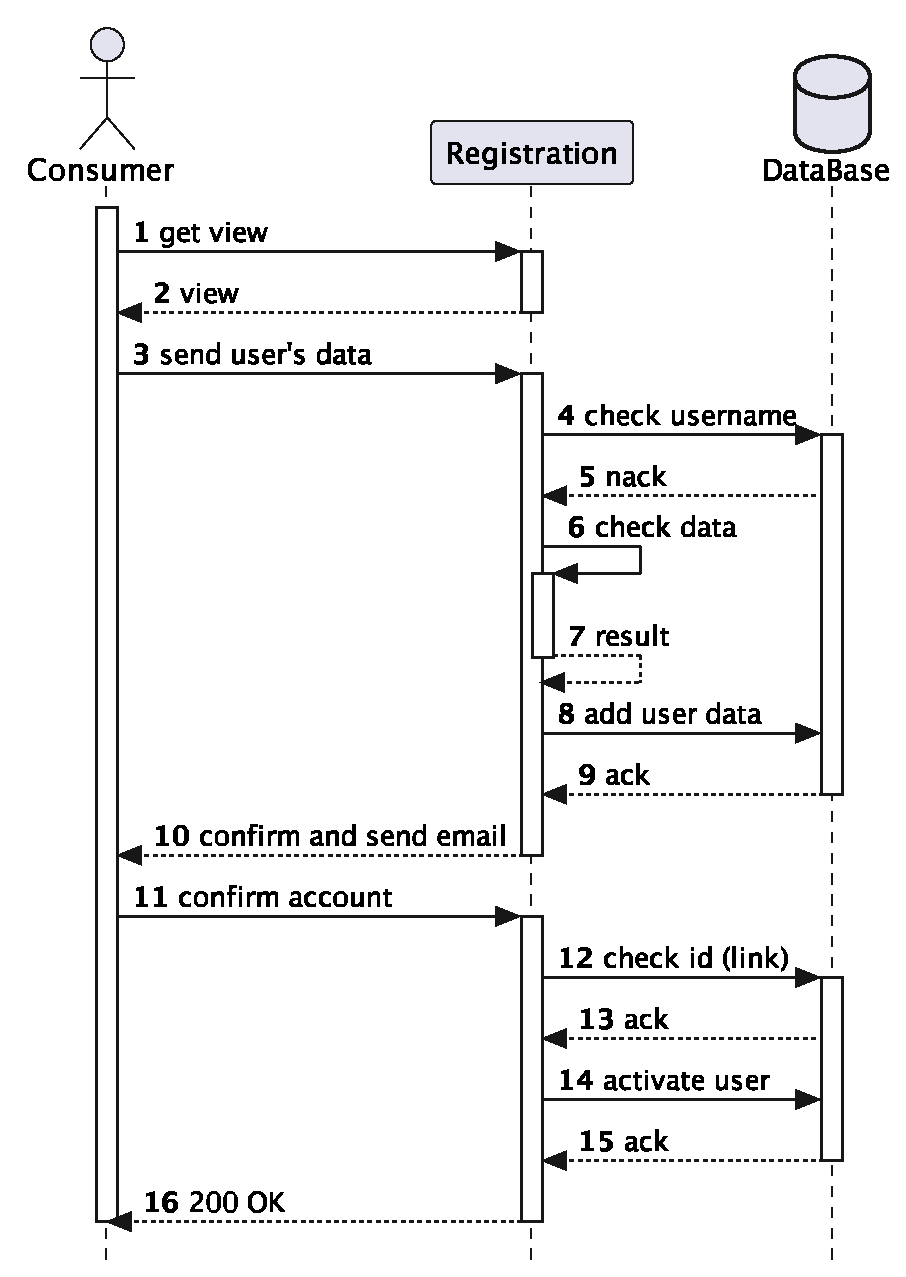
\includegraphics[width=0.46\columnwidth]{./images/diagrams/sequences/emsp/registration}
    \caption{registration of the eMSP user (consumer).}
\end{figure}

\pagebreak

\paragraph{eMSP | Login}

\begin{center}
    \begin{tabular}{ | >{\arraybackslash}m{0.17\columnwidth} | >{\arraybackslash}m{0.77\columnwidth} | }
        \hline
        \textbf{Identifier} & \showUC{uc:e:login} \\
        \hline
        \textbf{Actor} & Consumer (end user) \\
        \hline
        \textbf{Entry condition} & The user is already registered \\
        \hline
        \textbf{Event flow} & \medskip\parbox[b][][b]{0.76\columnwidth}{
            \begin{enumerate}[nosep, leftmargin=*]
                \item The user opens the application or webpage
                \item The user fills out the login form
                \item The system checks the inserted data
                \item The system logs in the user sending back a token with all the information
            \end{enumerate}
        } \\
        \hline
        \textbf{Exit condition} & The process ends without errors and the token is sent \\
        \hline
        \textbf{Exceptions} & \medskip\parbox[b][][b]{0.76\columnwidth}{
            \begin{itemize}[nosep, leftmargin=*]
                \item The inserted username corresponds to a non-activated account
                \item The username doesn't exist
                \item The password hash doesn't coincide
            \end{itemize}
        } \\
        \hline
    \end{tabular}
\end{center}

\begin{figure}[h!]
    \centering
    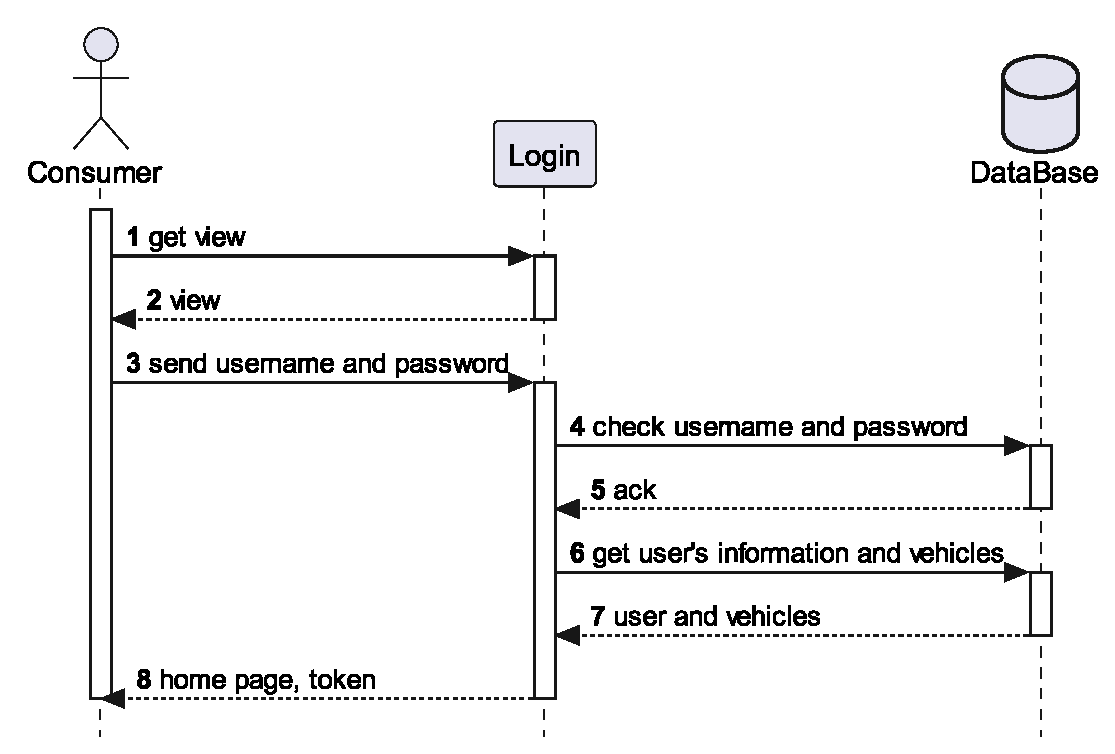
\includegraphics[width=0.62\columnwidth]{./images/diagrams/sequences/emsp/login}
    \caption{login of the eMSP user (consumer).}
\end{figure}

Please, note that the token present in the scheme is to be intended like a JWT with all the information of the user (which can fit into the token because of their small size) that has to be sent every time. This explains why certain pieces of information are not queried every time they are needed.

\pagebreak

\paragraph{eMSP | Vehicles editing}

\begin{center}
    \begin{tabular}{ | >{\arraybackslash}m{0.17\columnwidth} | >{\arraybackslash}m{0.77\columnwidth} | }
        \hline
        \textbf{Identifier} & \showUC{uc:e:vehicles} \\
        \hline
        \textbf{Actor} & Consumer (end user) \\
        \hline
        \textbf{Entry condition} & The user needs to add/remove/edit one or more associated vehicles \\
        \hline
        \textbf{Event flow} & \medskip\parbox[b][][b]{0.76\columnwidth}{
            \begin{enumerate}[nosep, leftmargin=*]
                \item The user opens the list of vehicles
                \item The user adds a new vehicle (inserting all the data) or clicks on one
                \item If the user clicks on a vehicle, he can choose to edit or remove it
                \item The system confirms the operation, sends back an updated token, and updates any future reservation (deleting it if the vehicle is deleted or editing it with the new certificate)
            \end{enumerate}
        } \\
        \hline
        \textbf{Exit condition} & The process ends without errors \\
        \hline
        \textbf{Exceptions} & \medskip\parbox[b][][b]{0.76\columnwidth}{
            \begin{itemize}[nosep, leftmargin=*]
                \item The user tries to remove some information from a vehicle while editing
            \end{itemize}
        } \\
        \hline
        \textbf{Special requests} & If the user wants to add a new vehicle or to change the certificate of any, s/he has to be able to upload the certificate \\
        \hline
    \end{tabular}
\end{center}

\begin{figure}[h!]
    \centering
    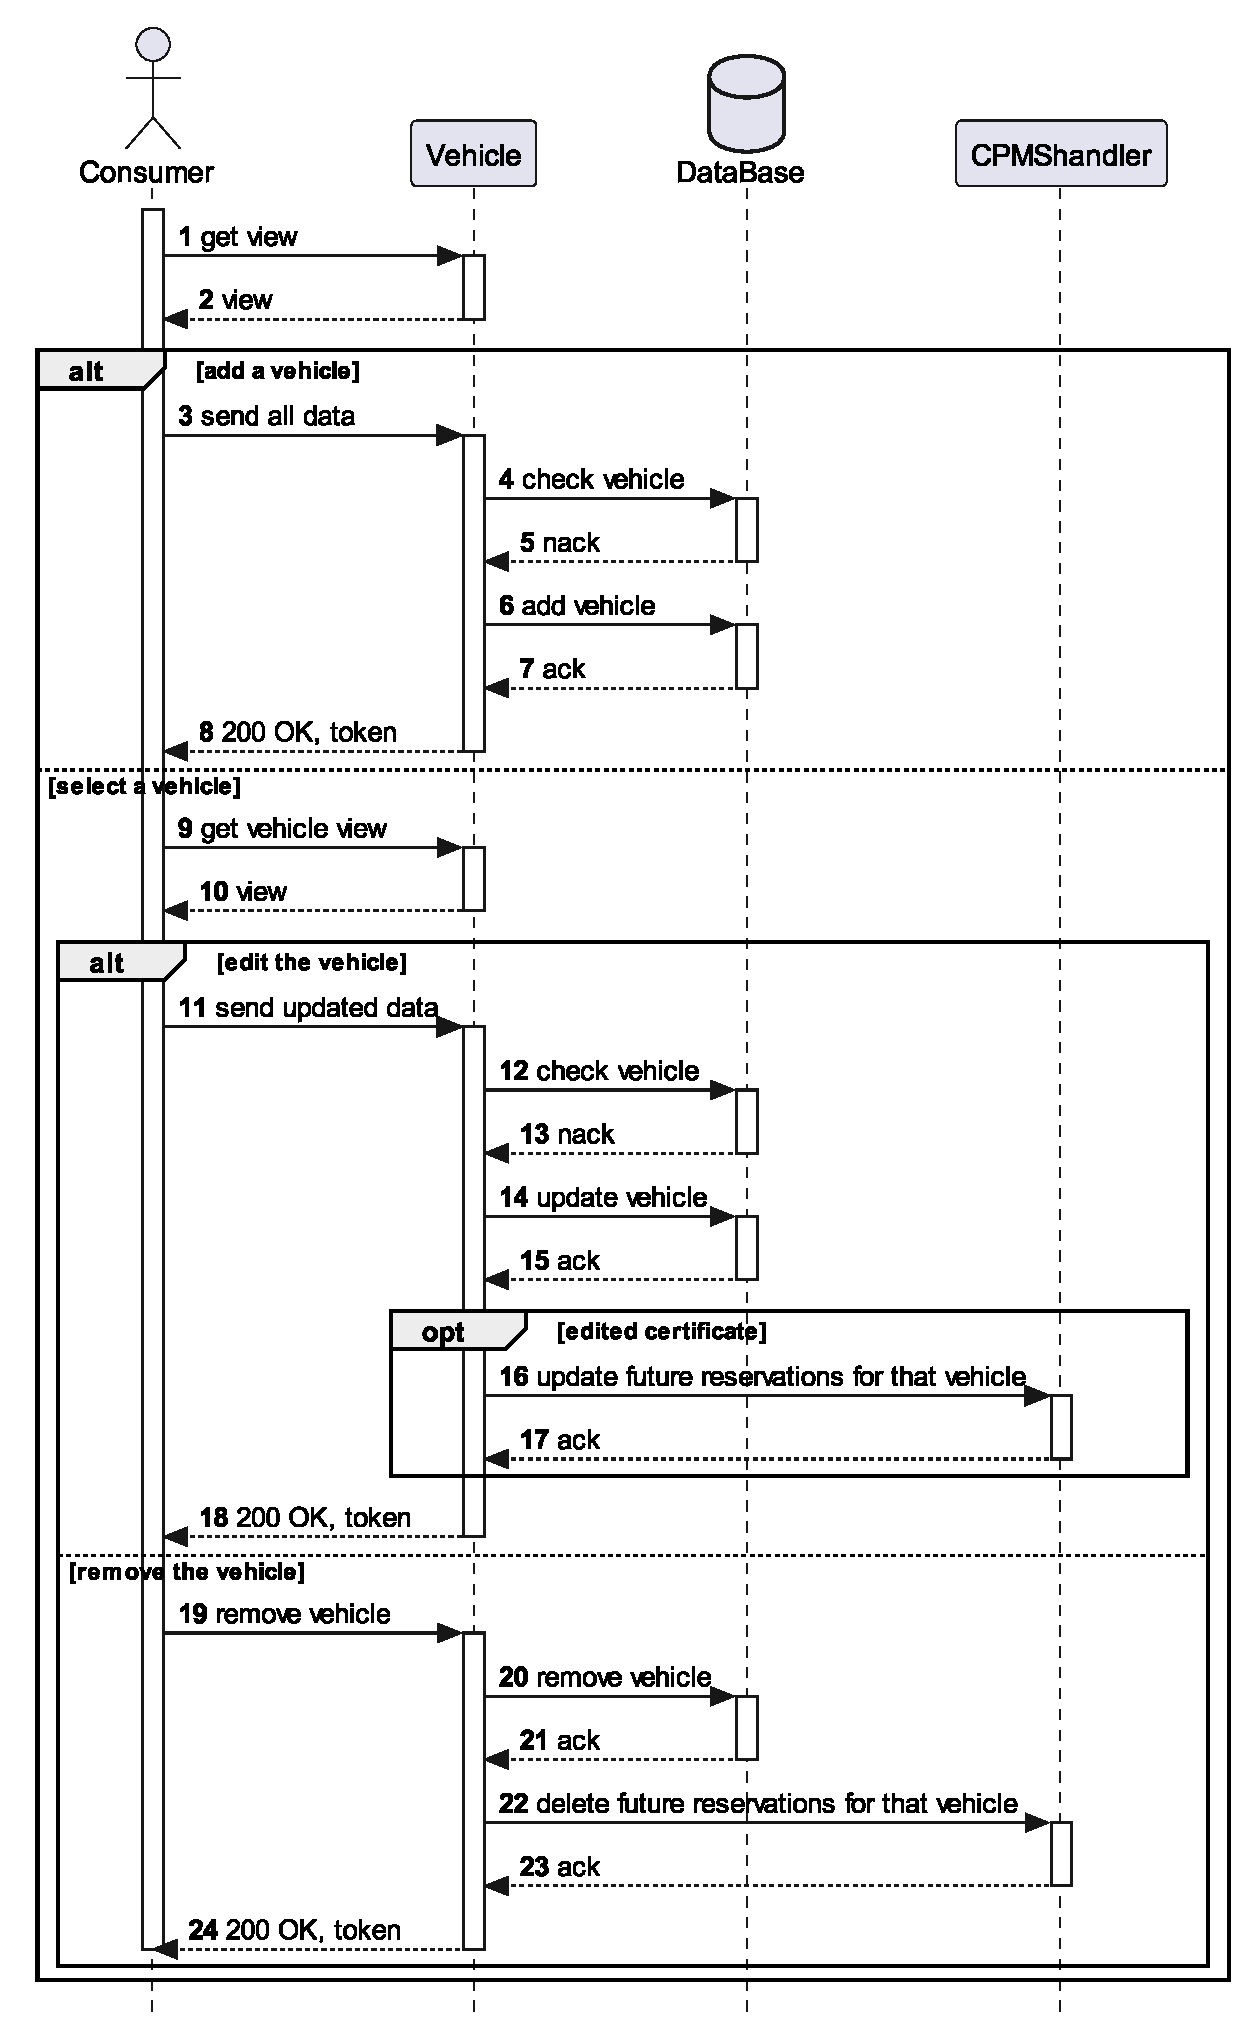
\includegraphics[width=0.59\columnwidth]{./images/diagrams/sequences/emsp/vehicles}
    \caption{the user manages his/her vehicles.}
\end{figure}

\pagebreak

\paragraph{eMSP | Look for nearby stations}

\begin{center}
    \begin{tabular}{ | >{\arraybackslash}m{0.17\columnwidth} | >{\arraybackslash}m{0.77\columnwidth} | }
        \hline
        \textbf{Identifier} & \showUC{uc:e:stations_lookup} \\
        \hline
        \textbf{Actor} & Consumer (end user) \\
        \hline
        \textbf{Entry condition} & The user is already logged in \\
        \hline
        \textbf{Event flow} & \medskip\parbox[b][][b]{0.76\columnwidth}{
            \begin{enumerate}[nosep, leftmargin=*]
                \item The user opens the map page (if s/he selects the favorites, skips to the last point)
                \item The user activates the geolocalization or searches for a place
                \item If wanted, the user clicks on the list view (s/he can switch at any time)
                \item If the user is in the list view, s/he can sort the stations based on some parameters
                \item The user opens the details of the charging station, eventually toggling favorite
            \end{enumerate}
        } \\
        \hline
        \textbf{Exit condition} & The process ends without errors \\
        \hline
        \textbf{Exceptions} & \medskip\parbox[b][][b]{0.76\columnwidth}{
            \begin{itemize}[nosep, leftmargin=*]
                \item The user inserts a nonexistent location
            \end{itemize}
        } \\
        \hline
    \end{tabular}
\end{center}

\begin{figure}[h!]
    \centering
    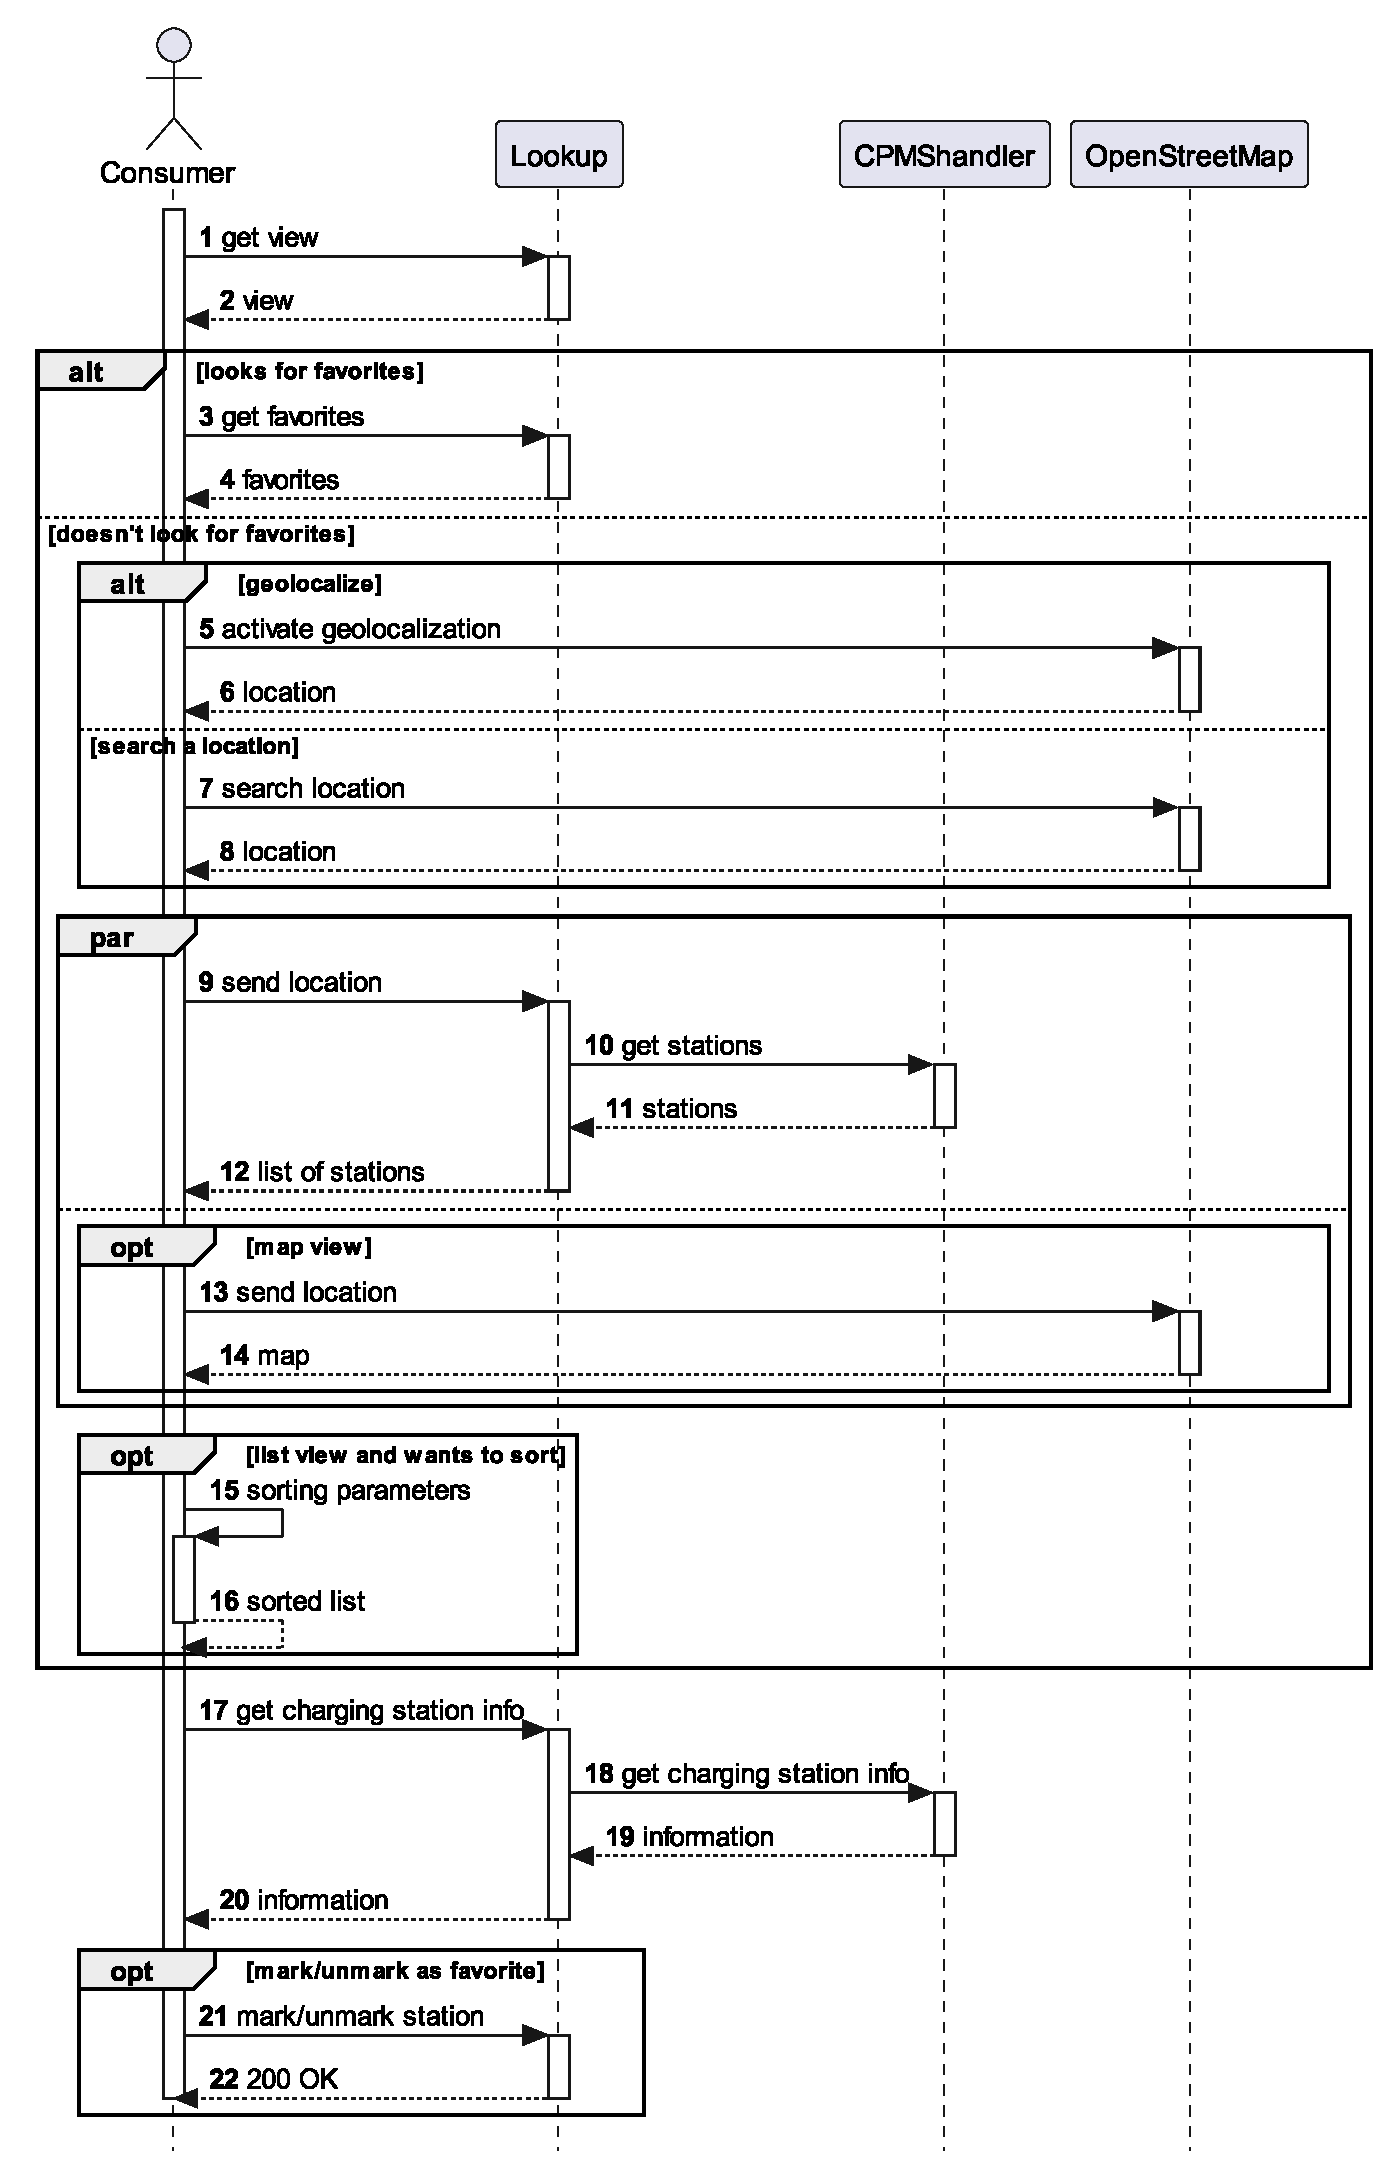
\includegraphics[width=0.67\columnwidth]{./images/diagrams/sequences/emsp/lookup}
    \caption{the user looks for a charging station and marks/unmarks it as \doublequotes{favorite}.}
\end{figure}

\pagebreak

\paragraph{eMSP | Book a charge}

\begin{center}
    \begin{tabular}{ | >{\arraybackslash}m{0.17\columnwidth} | >{\arraybackslash}m{0.77\columnwidth} | }
        \hline
        \textbf{Identifier} & \showUC{uc:e:book} \\
        \hline
        \textbf{Actor} & Consumer (end user) \\
        \hline
        \textbf{Entry condition} & The user has already opened the information of a charging station \\
        \hline
        \textbf{Event flow} & \medskip\parbox[b][][b]{0.76\columnwidth}{
            \begin{enumerate}[nosep, leftmargin=*]
                \item The user opens the book functionality
                \item The user selects the vehicle to charge (only if more than one)
                \item The user selects some available slots
                \item The system notifies the user of the successful operation and sends all the details
            \end{enumerate}
        } \\
        \hline
        \textbf{Exit condition} & The process ends without errors \\
        \hline
        \textbf{Exceptions} & \medskip\parbox[b][][b]{0.76\columnwidth}{
            \begin{itemize}[nosep, leftmargin=*]
                \item The user has no associated vehicle
                \item There are no available slots for that charging station and socket
                \item The user selects a duration that exceeds the maximum duration for that slot
                \item Some other user, meanwhile, has booked even a small part of the selected slot
            \end{itemize}
        } \\
        \hline
    \end{tabular}
\end{center}

\begin{figure}[h!]
    \centering
    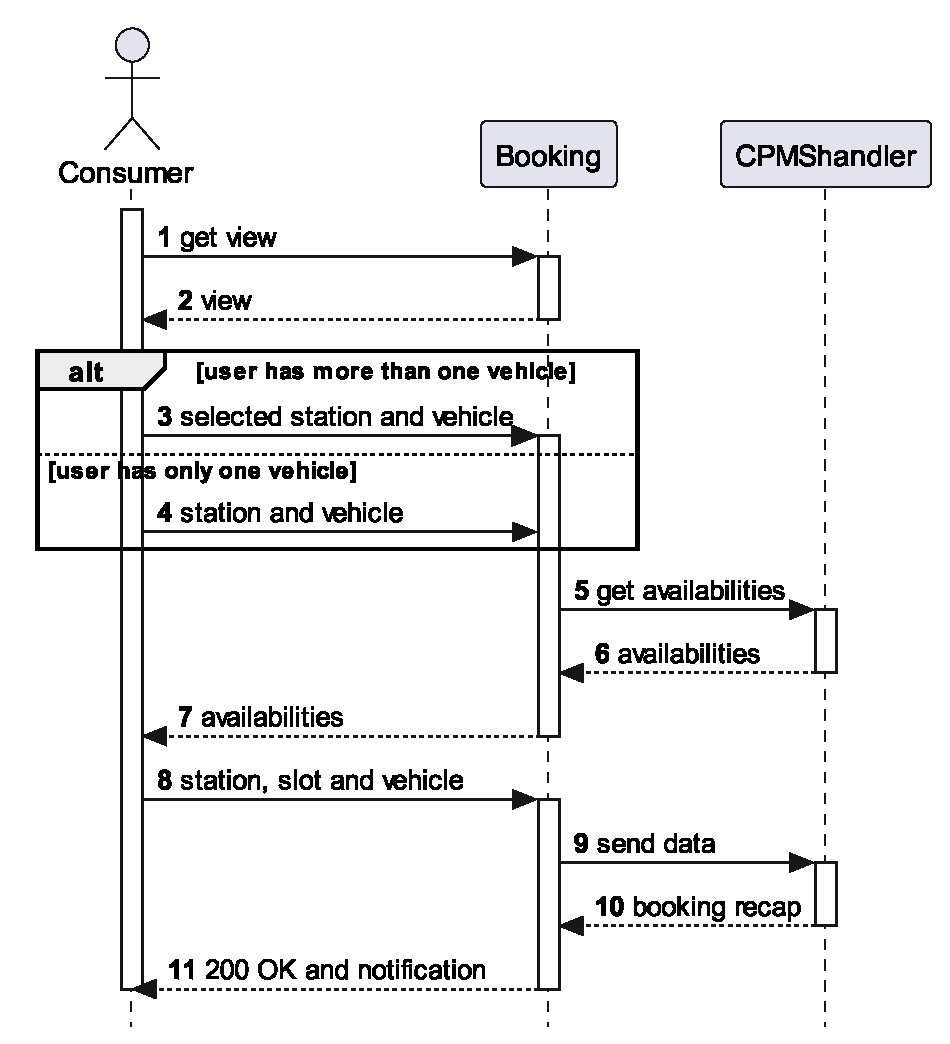
\includegraphics[width=0.5\columnwidth]{./images/diagrams/sequences/emsp/book}
    \caption{the user books a charge.}
\end{figure}

\pagebreak

\paragraph{eMSP | Edit/delete a reservation}

\begin{center}
    \begin{tabular}{ | >{\arraybackslash}m{0.17\columnwidth} | >{\arraybackslash}m{0.77\columnwidth} | }
        \hline
        \textbf{Identifier} & \showUC{uc:e:edit} \\
        \hline
        \textbf{Actor} & Consumer (end user) \\
        \hline
        \textbf{Entry condition} & The user has already booked a charge and needs to edit or delete it \\
        \hline
        \textbf{Event flow} & \medskip\parbox[b][][b]{0.76\columnwidth}{
            \begin{enumerate}[nosep, leftmargin=*]
                \item The user accesses the list of future charges
                \item The user selects a charge
                \item The user edits (following steps 2-4 of \refUC{uc:e:book}) or deletes it
                \item The system notifies the change
            \end{enumerate}
        } \\
        \hline
        \textbf{Exit condition} & The process ends without errors \\
        \hline
        \textbf{Exceptions} & \medskip\parbox[b][][b]{0.76\columnwidth}{
            \begin{itemize}[nosep, leftmargin=*]
                \item The user tries to delete a past or current charge
                \item An exception from the booking process ones (\refUC{uc:e:book}) arises
            \end{itemize}
        } \\
        \hline
    \end{tabular}
\end{center}

\begin{figure}[h!]
    \centering
    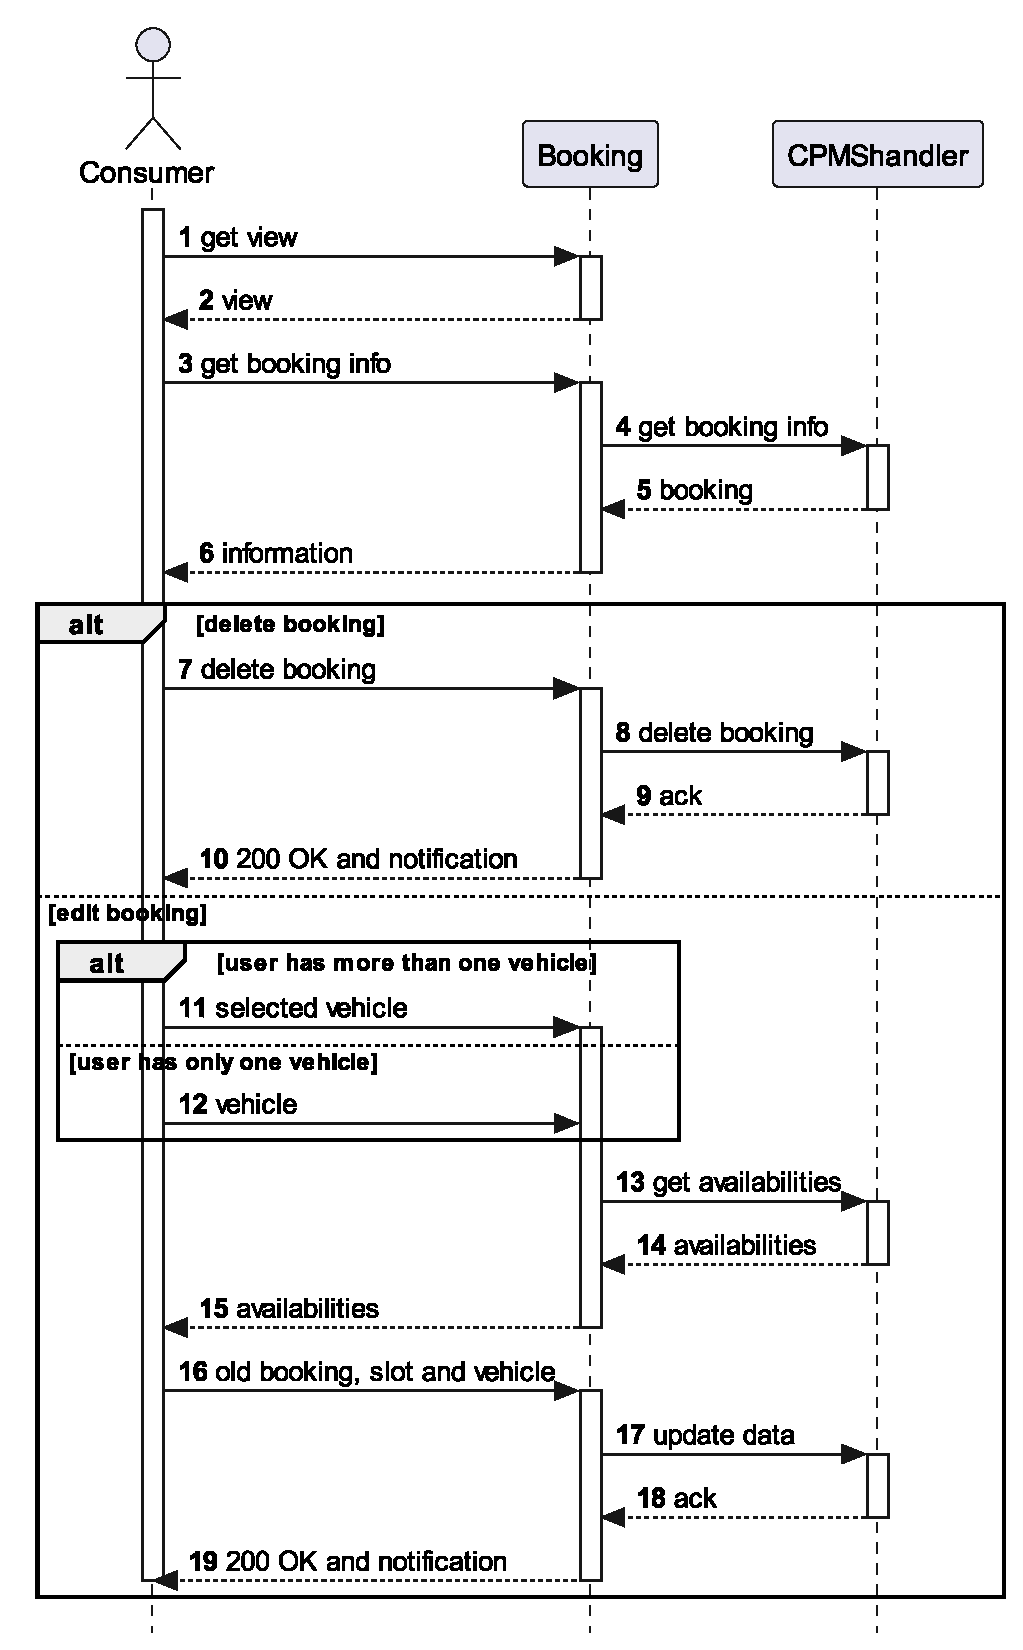
\includegraphics[width=0.57\columnwidth]{./images/diagrams/sequences/emsp/edit}
    \caption{the user edits or removes a booked charge.}
\end{figure}

\pagebreak

\paragraph{eMSP | Get notified}

\begin{center}
    \begin{tabular}{ | >{\arraybackslash}m{0.17\columnwidth} | >{\arraybackslash}m{0.77\columnwidth} | }
        \hline
        \textbf{Identifier} & \showUC{uc:e:notification} \\
        \hline
        \textbf{Actor} & Consumer (end user) \\
        \hline
        \textbf{Entry condition} & The system is informed about an important fact for the user (assigned socket, end of charge, or payment result) \\
        \hline
        \textbf{Event flow} & \medskip\parbox[b][][b]{0.76\columnwidth}{
            \begin{enumerate}[nosep, leftmargin=*]
                \item The system checks the user's notification preferences
                \item The system notifies the user
            \end{enumerate}
        } \\
        \hline
        \textbf{Exit condition} & The notification is sent to the user \\
        \hline
    \end{tabular}
\end{center}

\begin{figure}[h!]
    \centering
    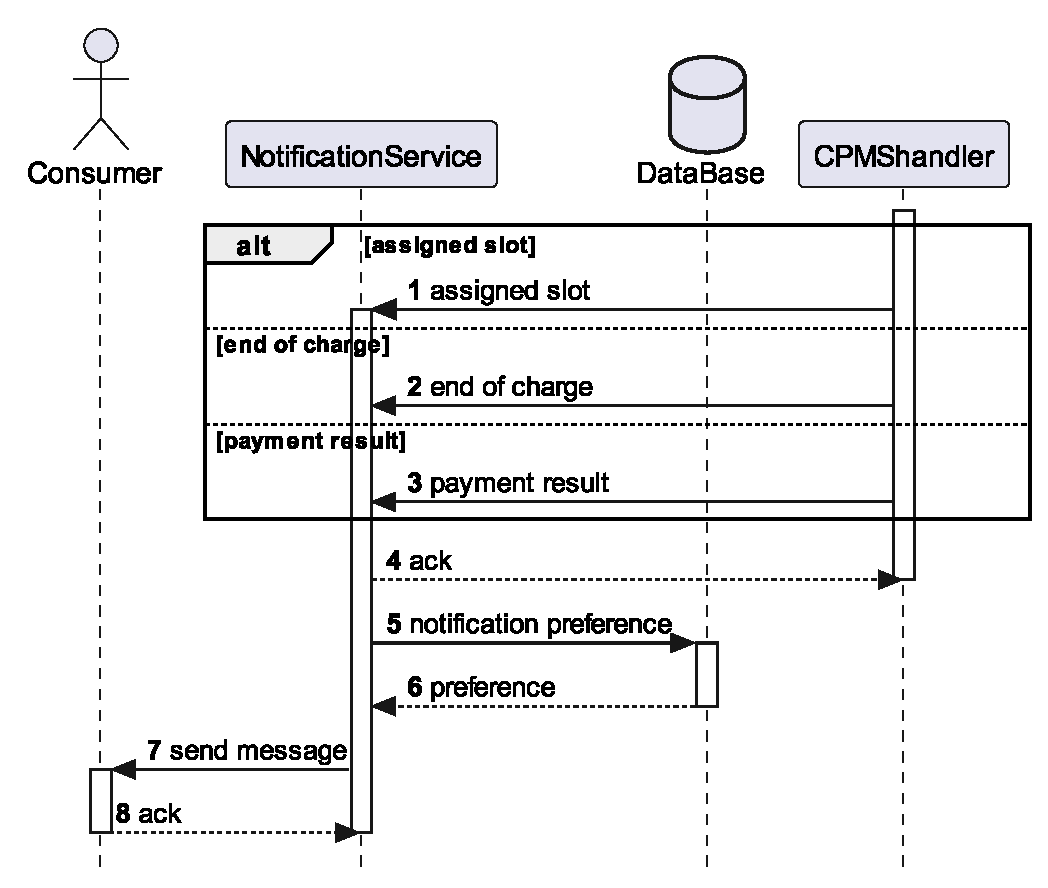
\includegraphics[width=0.55\columnwidth]{./images/diagrams/sequences/emsp/notification}
    \caption{the system notifies the user about an important fact from the CPMS.}
\end{figure}

Since these three cases are close to each other, they are represented together in the same use case.

\pagebreak

\paragraph{eMSP | Pay for the obtained service}

\begin{center}
    \begin{tabular}{ | >{\arraybackslash}m{0.17\columnwidth} | >{\arraybackslash}m{0.77\columnwidth} | }
        \hline
        \textbf{Identifier} & \showUC{uc:e:payment} \\
        \hline
        \textbf{Actor} & Consumer (end user) \\
        \hline
        \textbf{Entry condition} & After completing a charge, the user has to pay for it \\
        \hline
        \textbf{Event flow} & \medskip\parbox[b][][b]{0.76\columnwidth}{
            \begin{enumerate}[nosep, leftmargin=*]
                \item The user selects the charge to pay
                \item The system redirects the user to the payment page
                \item The user inserts the data
                \item The system confirms the payment and notifies the CPMS and the user
            \end{enumerate}
        } \\
        \hline
        \textbf{Exit condition} & The process ends without errors \\
        \hline
        \textbf{Exceptions} & \medskip\parbox[b][][b]{0.76\columnwidth}{
            \begin{itemize}[nosep, leftmargin=*]
                \item The user inserts wrong payment data
            \end{itemize}
        } \\
        \hline
        \textbf{Special requests} & The user has a valid payment method \\
        \hline
    \end{tabular}
\end{center}

\begin{figure}[h!]
    \centering
    
\includegraphics[width=0.66\columnwidth]{./images/diagrams/sequences/emsp/payment}
    \caption{the user pays for the charge.}
\end{figure}

Similar to this, the in-loco payment requires the user to insert his/her payment data (or to use a payment card, according to how it's implemented) and in this case it's the CPMS who notifies the eMSP, and not the other way round.

\pagebreak

\paragraph{CPMS | Login}

\begin{center}
    \begin{tabular}{ | >{\arraybackslash}m{0.17\columnwidth} | >{\arraybackslash}m{0.77\columnwidth} | }
        \hline
        \textbf{Identifier} & \showUC{uc:c:login} \\
        \hline
        \textbf{Actor} & CPO allowed user \\
        \hline
        \textbf{Entry condition} &  The user is at the login page in the website\\
        \hline
        \textbf{Event flow} & \medskip\parbox[b][][b]{0.76\columnwidth}{
            \begin{enumerate}[nosep, leftmargin=*]
                \item The user enters login data
                \item The system checks if input data matches database content
                \item The system queries the DBMS for home page data
                \item The system sends back the home page with all relevant information 
            \end{enumerate}
        } \\
        \hline
        \textbf{Exit condition} & The process ends without errors \\
        \hline
        \textbf{Exceptions} & \medskip\parbox[b][][b]{0.76\columnwidth}{
            \begin{itemize}[nosep, leftmargin=*]
                \item Missing or wrong input data is sent from the user
            \end{itemize}
        } \\
        \hline
    \end{tabular}
\end{center}

\begin{figure}[h!]
    \centering
    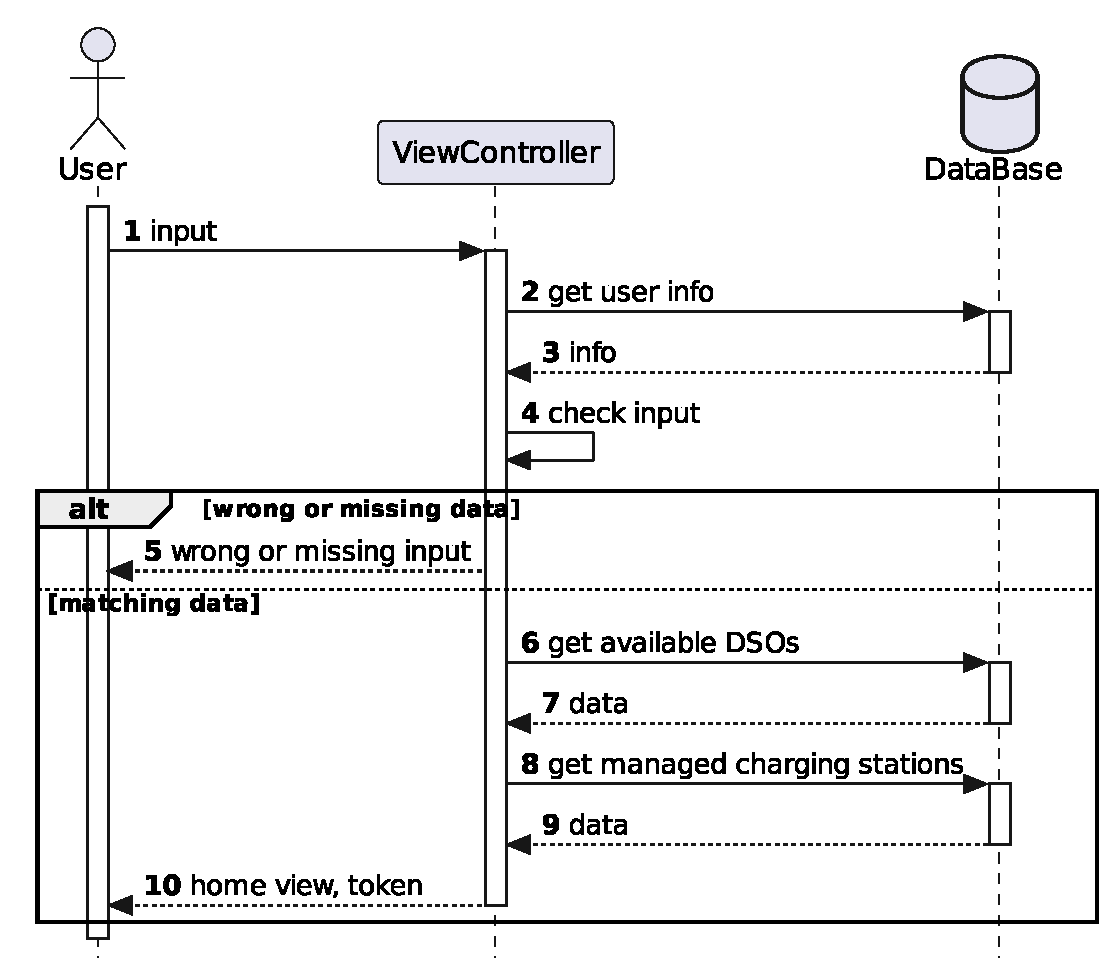
\includegraphics[width=0.65\columnwidth]{./images/diagrams/sequences/cpms/login}
    \caption{login of a registered CPO user.}
\end{figure}

\pagebreak

\paragraph{CPMS | Check charging station status}


\begin{center}
    \begin{tabular}{ | >{\arraybackslash}m{0.17\columnwidth} | >{\arraybackslash}m{0.77\columnwidth} | }
        \hline
        \textbf{Identifier} & \showUC{uc:c:infStation} \\
        \hline
        \textbf{Actor} & CPO allowed user \\
        \hline
        \textbf{Entry condition} &  The user is at the home page in the website\\
        \hline
        \textbf{Event flow} & \medskip\parbox[b][][b]{0.76\columnwidth}{
            \begin{enumerate}[nosep, leftmargin=*]
                \item The user selects a charging station
                \item The user selects \doublequotes{Check status}
                \item The system queries the DBMS for all relevant information
                \item The DBMS returns all relevant information
                \item The system sends back the new page with all relevant information 
                \item The system periodically sends new information to the website
            \end{enumerate}
        } \\
        \hline
        \textbf{Exit condition} & The process ends without errors \\
        \hline
        \textbf{Exceptions} & \medskip\parbox[b][][b]{0.76\columnwidth}{
            \begin{itemize}[nosep, leftmargin=*]
                \item A non-existing charging station is selected
                \item The selected charging station is not managed by the user
            \end{itemize}
        } \\
        \hline
    \end{tabular}
\end{center}

\begin{figure}[h!]
    \centering
    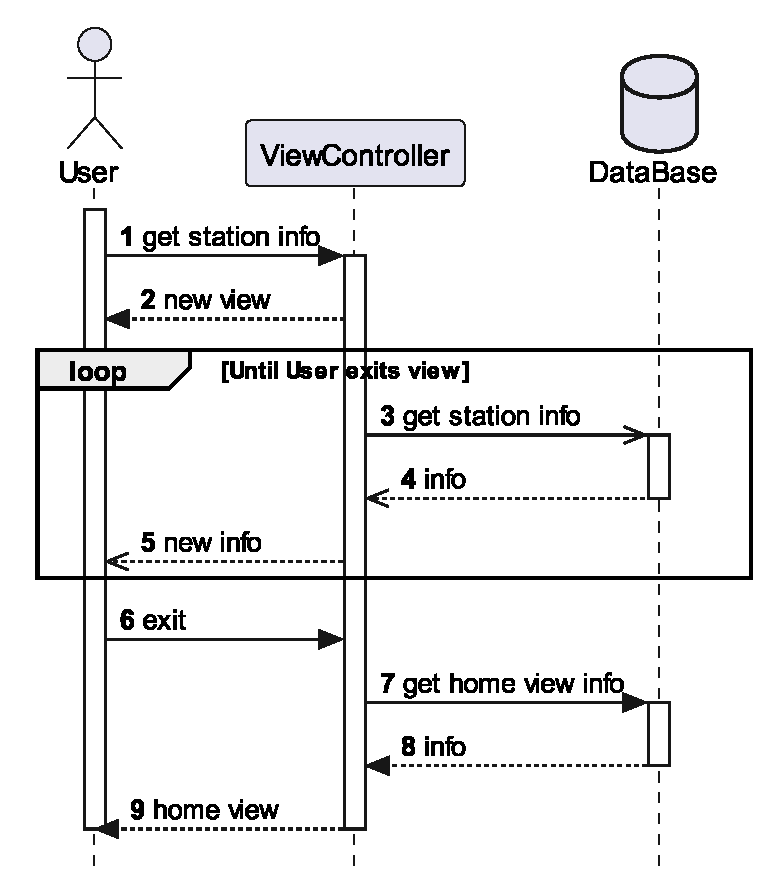
\includegraphics[width=0.50\columnwidth]{./images/diagrams/sequences/cpms/infStation}
    \caption{change view from the home page to charging station info.}
\end{figure}

As stated in requirement \refR{r:c:periodical_updates}, the system periodically has to update the database with information regarding all changing parameters coming from charging stations. These include the station's battery levels, incoming energy from the solar panels, occupied columns in the station, and eventually more data. This allows the view controller to simply fetch data from the database, instead of intercepting all data streams, to communicate to the website in the corresponding views.

\pagebreak

\paragraph{CPMS | Change energy mix}

\begin{center}
    \begin{tabular}{ | >{\arraybackslash}m{0.17\columnwidth} | >{\arraybackslash}m{0.77\columnwidth} | }
        \hline
        \textbf{Identifier} & \showUC{uc:c:changeMix} \\
        \hline
        \textbf{Actor} & CPO allowed user \\
        \hline
        \textbf{Entry condition} & The user is at the home page in the website \\
        \hline
        \textbf{Event flow} & \medskip\parbox[b][][b]{0.76\columnwidth}{
            \begin{enumerate}[nosep, leftmargin=*]
                \item The user selects \doublequotes{Change energy mix}
                \item The user defines a new energy mix
                \item The system communicates the new energy mix to the charging station
                \item The charging station communicates the components the change
            \end{enumerate}
        } \\
        \hline
        \textbf{Exit condition} & A new energy mix is defined without errors, the user is notified \\
        \hline
        \textbf{Exceptions} & \medskip\parbox[b][][b]{0.76\columnwidth}{
            \begin{itemize}[nosep, leftmargin=*]
                \item The new energy mix could not be attained 
                \item The database could not be updated 
                \item The user could not be notified 
            \end{itemize}
        } \\
        \hline
        \textbf{Special requests} & The user has to input a reasonable energy mix \\
        \hline
    \end{tabular}
\end{center}

\begin{figure}[h!]
    \centering
    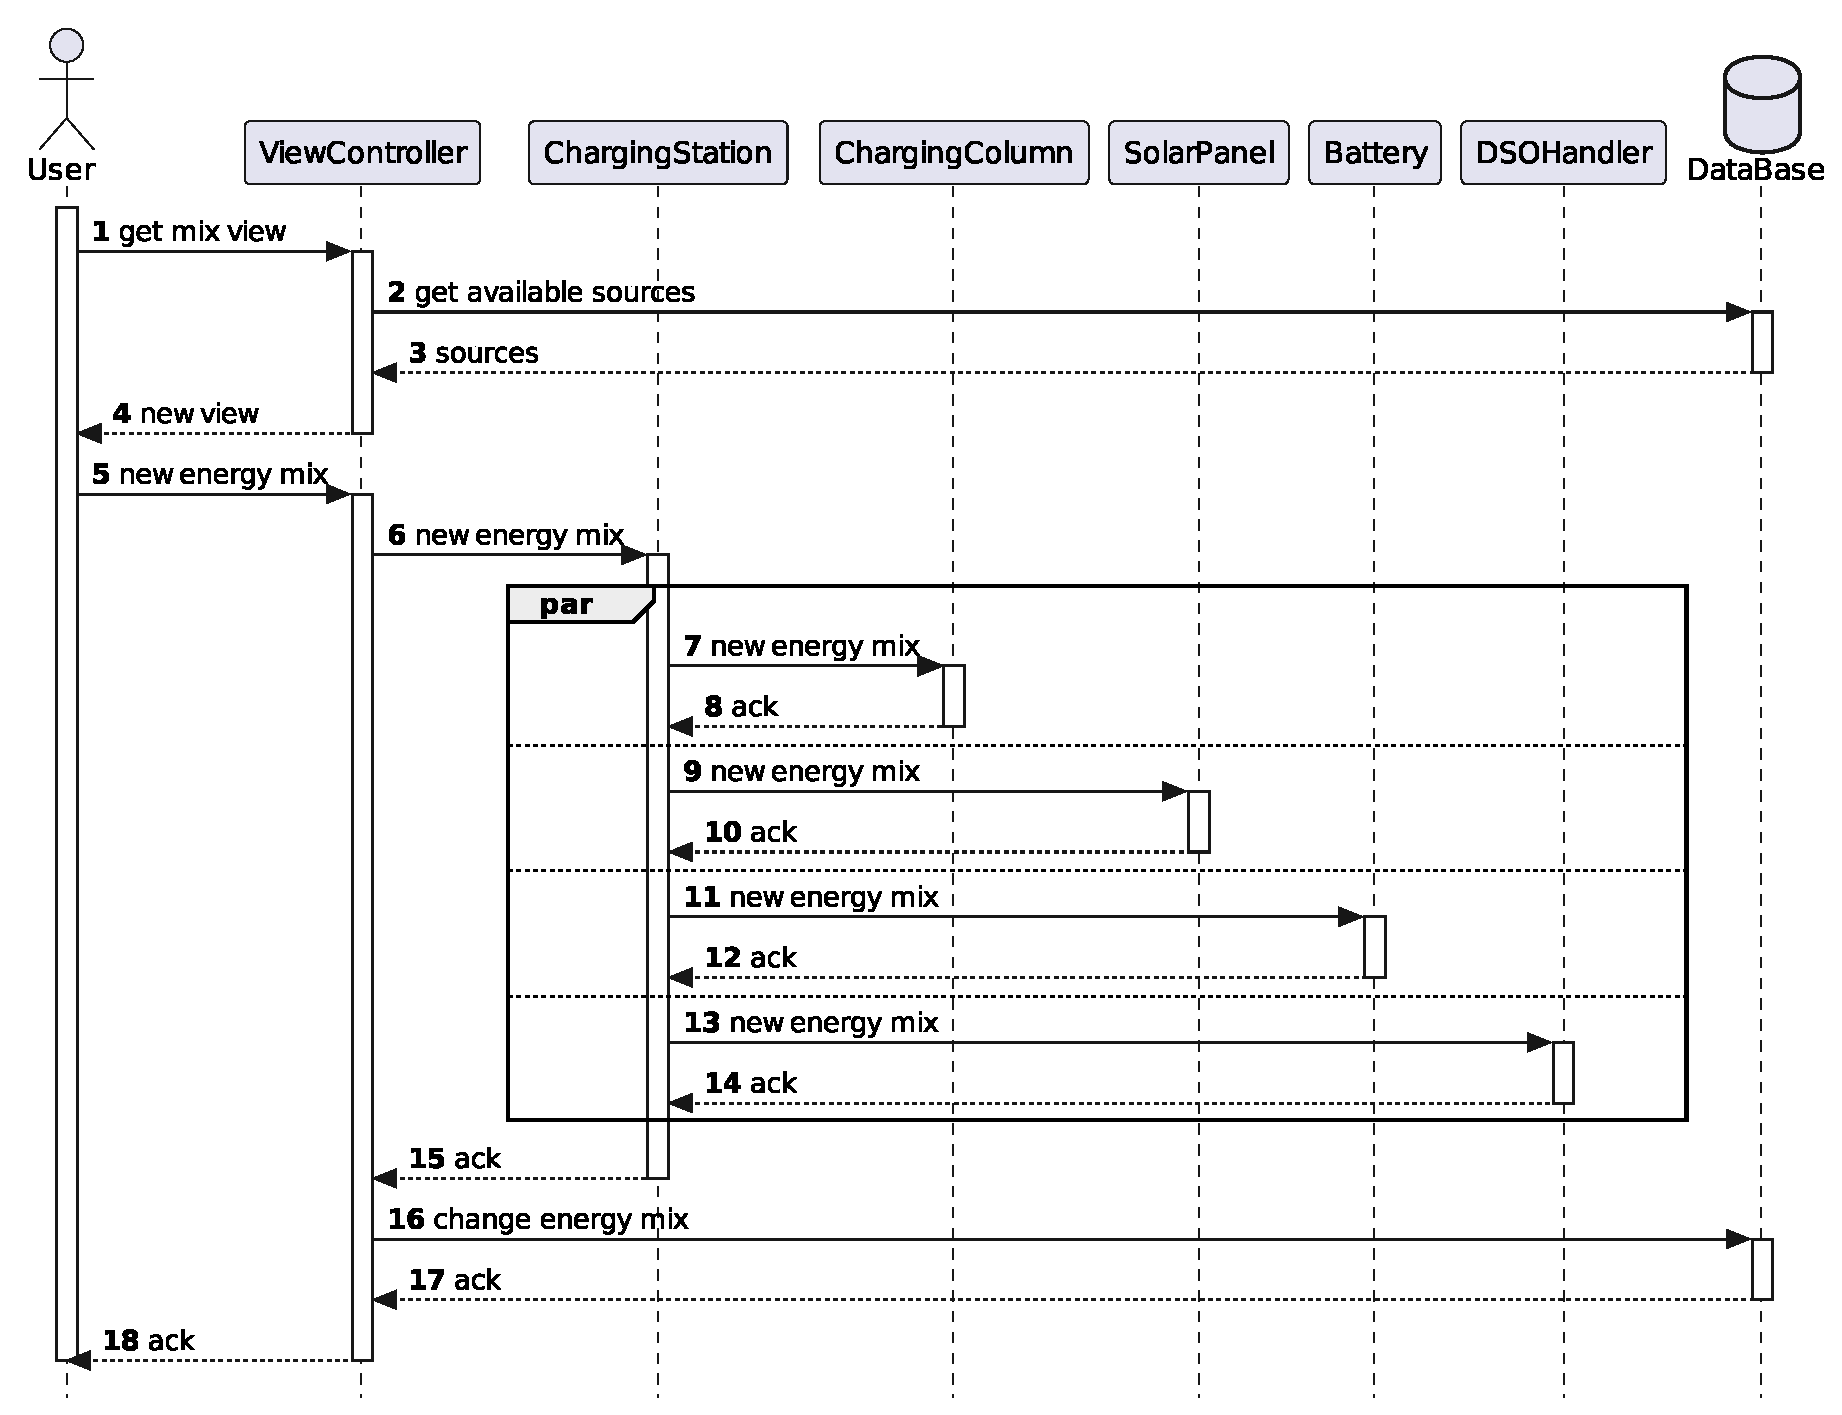
\includegraphics[width=1\columnwidth]{./images/diagrams/sequences/cpms/energyMix}
    \caption{user changing energy mix of a charging station.}
\end{figure}

\pagebreak

\paragraph{CPMS | Manage DSO choice}

\begin{center}
    \begin{tabular}{ | >{\arraybackslash}m{0.17\columnwidth} | >{\arraybackslash}m{0.77\columnwidth} | }
        \hline
        \textbf{Identifier} & \showUC{uc:c:DSO} \\
        \hline
        \textbf{Actor} & CPO allowed user \\
        \hline
        \textbf{Entry condition} & The user is at the home page in the website \\
        \hline
        \textbf{Event flow} & \medskip\parbox[b][][b]{0.76\columnwidth}{
            \begin{enumerate}[nosep, leftmargin=*]
                \item The user selects a charging station
                \item The user selects \doublequotes{Available DSO}
                \item The system sends a new DSO view
                \item The user selects a DSO
                \item The system starts using the selected DSO in the charging station
            \end{enumerate}
        } \\
        \hline
        \textbf{Exit condition} & The DSO is being used in the charging station and the user is notified \\
        \hline
        \textbf{Exceptions} & \medskip\parbox[b][][b]{0.76\columnwidth}{
            \begin{itemize}[nosep, leftmargin=*]
                \item The DSO stops being available while the choice is being made
            \end{itemize}
        } \\
        \hline
    \end{tabular}
\end{center}

\begin{figure}[h!]
    \centering
    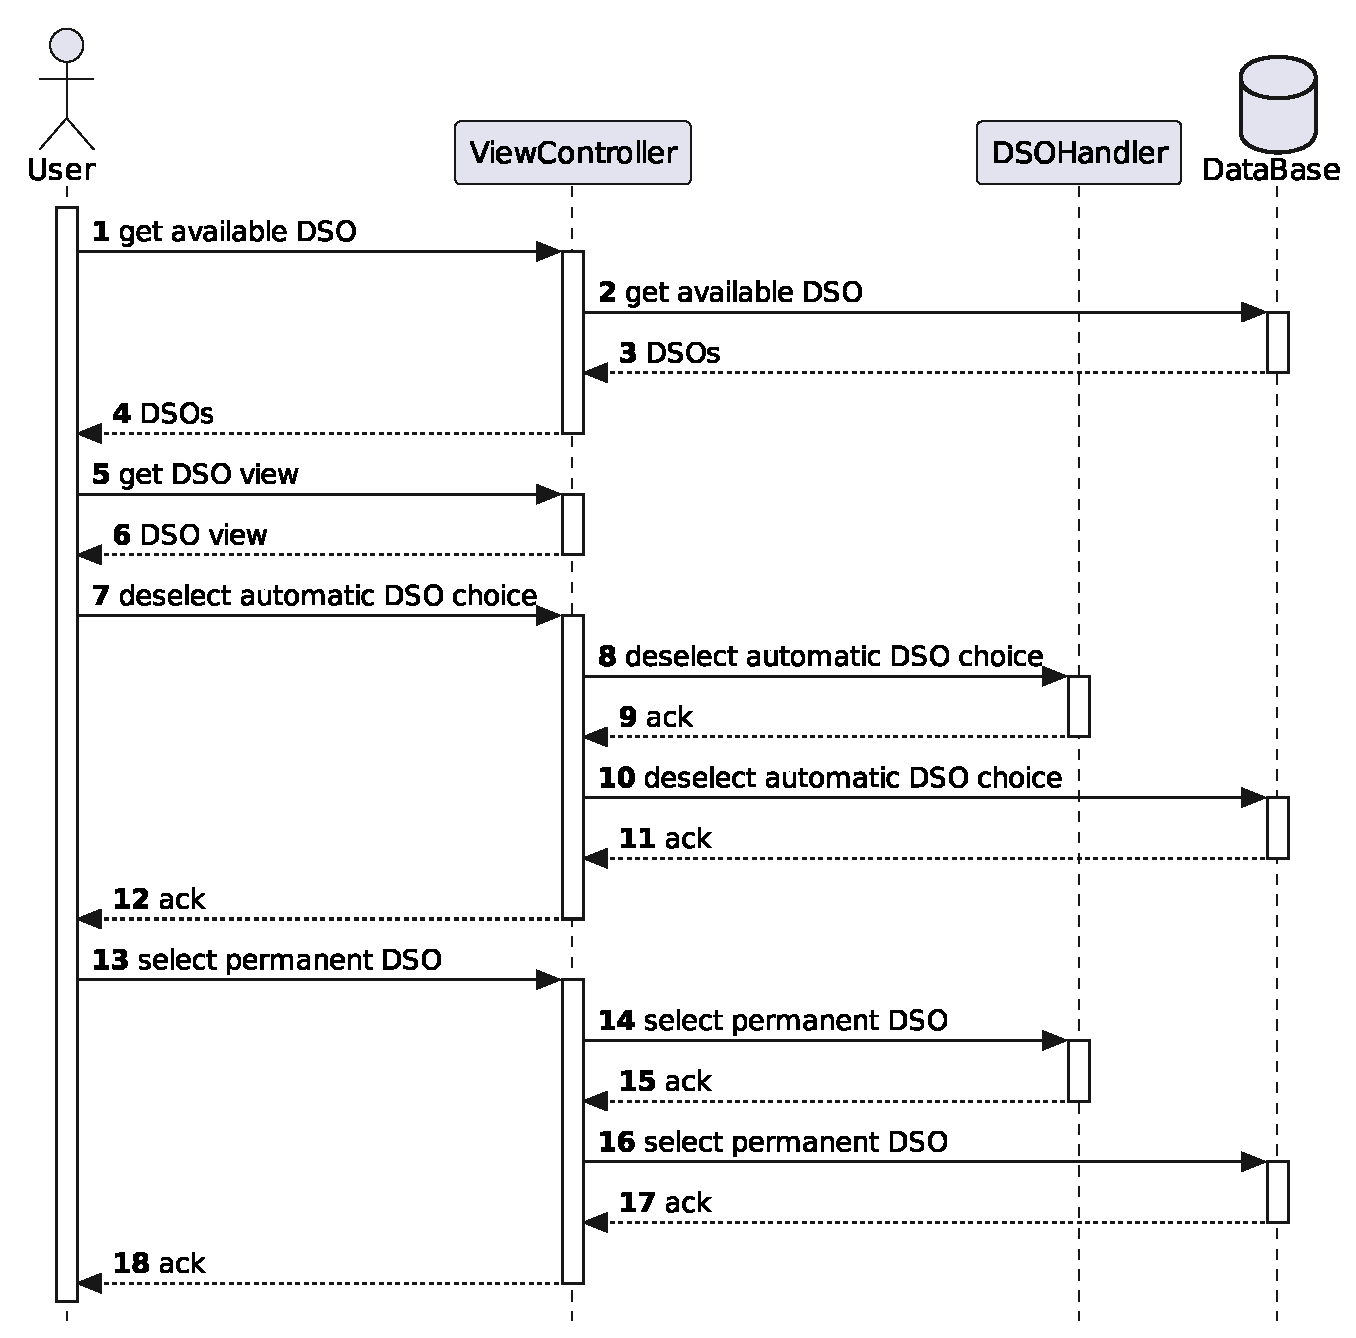
\includegraphics[width=0.85\columnwidth]{./images/diagrams/sequences/cpms/DSO}
    \caption{Caption}
\end{figure}

Instead of selecting a specific DSO, the user at the DSO view can also choose to activate/deactivate \doublequotes{Automatic DSO choice}, letting the system handle the DSO choice automatically or selecting the current DSO as permanent. In this view, it is also possible to modify the automatic payment method.

\pagebreak

\paragraph{CPMS | Create Special offer}

\begin{center}
    \begin{tabular}{ | >{\arraybackslash}m{0.17\columnwidth} | >{\arraybackslash}m{0.77\columnwidth} | }
        \hline
        \textbf{Identifier} & \showUC{uc:c:SpecialOffer} \\
        \hline
        \textbf{Actor} & CPO allowed user \\
        \hline
        \textbf{Entry condition} & The user is at the home page in the website \\
        \hline
        \textbf{Event flow} & \medskip\parbox[b][][b]{0.76\columnwidth}{
            \begin{enumerate}[nosep, leftmargin=*]
                \item The user selects \doublequotes{Special offers}
                \item The user selects \doublequotes{Create new special offer}
                \item The user inputs all the needed parameters
                \item The system creates a new special offer
            \end{enumerate}
        } \\
        \hline
        \textbf{Exit condition} & A new special offer is created \\
        \hline
        \textbf{Exceptions} & \medskip\parbox[b][][b]{0.76\columnwidth}{
            \begin{itemize}[nosep, leftmargin=*]
                \item Missing or wrong parameters
            \end{itemize}
        } \\
        \hline
    \end{tabular}
\end{center}

\begin{figure}[h!]
    \centering
    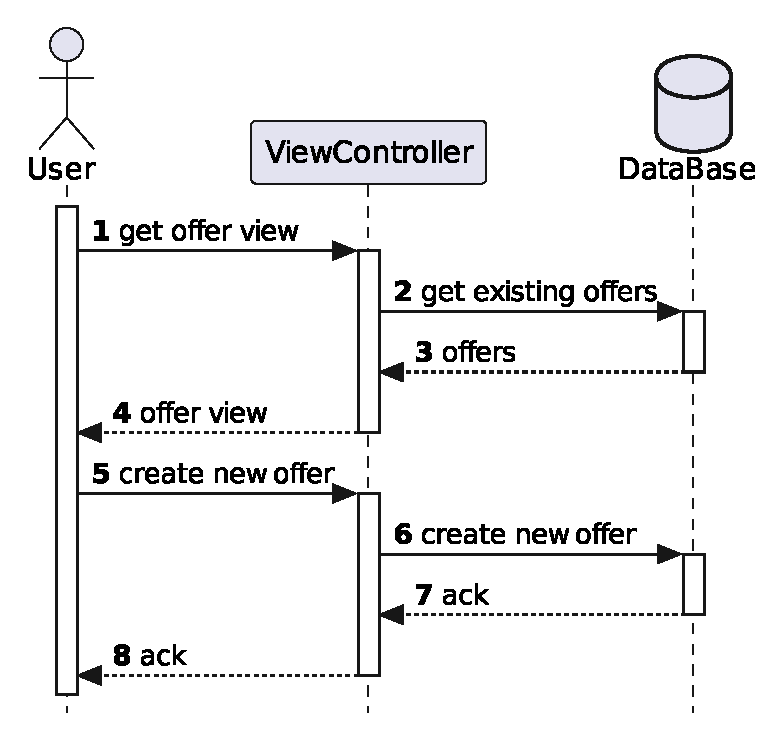
\includegraphics[width=0.45\columnwidth]{./images/diagrams/sequences/cpms/offers}
    \caption{a user creating a new special offer. In the special offer view users also see existing offers, and delete them if needed.}
\end{figure}

\pagebreak

\section{Performance requirements}

\paragraph{eMSP} The eMSP system should be generally responsive. It should provide answers to simple queries in less than 5 seconds, while more complex ones should complete in less than 30 seconds. If the system is directly interfacing with the user and the response isn't available after a couple of seconds, the frontend should display a loading indicator. A lower waiting time can be archived thanks to a proper database configuration and through the redundancy of components and data. The application performs much of the required computations on the backend, thus letting the application and the web interface only display the contents and doing some basic operations (sorting, checks\dots).

\paragraph{CPMS} Since the CPMS system is more geared towards monitoring, and eventually allows for some actions from the user, availability should be preferred over reliability. It's not essential that the system does not crush (although it is preferred), since all changes are immediately saved in permanent storage. It's more important that if the system crushes it can recover quickly, and all inputs are delivered as soon as possible and made permanent in the database storage. All the computation will take place on the servers of the system, which have to be replicated and distributed to better assert the desired availability and reach a consensus over the input received.

\section{Design constraints}

\subsection{Standards compliance}

Every system should correctly implement all the needed standard APIs for allowing interconnection with different pieces of software that expose those functionalities. Moreover, each system should be compliant with common payment APIs for managing user payments.

\subsection{Hardware limitations} \label{hwlimitations}

\paragraph{eMSP} For accessing the system, the user can use both the application which should be available in all the main mobile stores and should run on most of the devices present nowadays (e.g. an Android version greater or equal to 4.4 KitKat) or a browser which supports at least ES6 for correctly displaying all the views of the website.

\paragraph{CPMS} For accessing the system, any computer/laptop/tablet/phone with an installed web browser, connected to the internet, is sufficient, as a website is the sole user access point.

\section{Software system attributes}

\subsection{Reliability}

\paragraph{eMSP} The eMSP should be reliable, and even in case of failures, it should recover quickly. If downtimes, even if small, are frequent, this might make the user experience painful because of probably many failed requests.

\paragraph{CPMS} The CPMS website should be reliable enough to let users monitor and perform actions. Reliability is not to be preferred over availability. The CPMS servers on the other hand can be replicated to allow for higher reliability and protection of the data.

\subsection{Availability}

\paragraph{eMSP} The eMSP should be available 99\% of the time (about 361 days per year). Any longer unavailability period might encourage the user to move to some other competitor.

\paragraph{CPMS} The CPMS should be available 99.7\% of the time (about 364 days per year). Such a high availability is needed for the server to be responsive toward all end users, for better monitoring, and to secure that input actions are almost always registered.

\pagebreak

\subsection{Security}

\paragraph{eMSP} The eMSP should provide a high level of security for the information the users insert. Especially, the system must protect all the uploaded vehicles' information.

\paragraph{CPMS} The CPMS should provide a high level of security for the information the charging station dispatches. In particular, the system needs to be aware of \doublequotes{man in the middle} attacks where information coming from the stations is tampered with, which would result in incorrect automatic choices and eventually wrong information dispatched to the eMSP. Attention also should be paid to securing charging columns from possible manumissions in the validation of cars' certificates.

\subsection{Maintainability}

The system should follow basic design guidelines to make the whole system more maintainable. This will be described more deeply in the Design Document, but a general indication is to divide components into smaller ones, so that each one can do only a specific action, thus making the system easier to bring up and maintain, allowing also the maintenance of single components at a time.

\subsection{Portability}

\paragraph{eMSP} The backend should be able to run well on Linux systems, and it should be optimized to use all the standard Linux and POSIX features. The website should instead work well on all the major browsers, while the mobile application should be able to run on many architectures, allowing it to work on all the supported devices, as described in \reference{hwlimitations}.

\paragraph{CPMS} The backend should be able to run well on Linux systems, and it should be optimized to use all the standard Linux and POSIX features. The database system should be distributed for higher availability.

    \chapter{Formal Analysis} \label{alloy}

\section{Alloy code}

This section provides all the alloy code used to prove the correctness of the project. For a better reading, the code is subdivided into the different blocks it's composed.

\subsection{Entities}

\begin{minted}{Alloy}
// +--------------------------------------------+
// |                  General                   |
// +--------------------------------------------+

// Email address
sig Email {}

// Password
sig Password {}

// Booleans
abstract sig Boolean {}
lone sig True extends Boolean {}
lone sig False extends Boolean {}

// Date time, represented as an integer
sig DateTime {
    time: one Int
} {
    time >= 0
}

// Global time
lone sig GlobalTime {
    time: one DateTime
}

// +--------------------------------------------+
// |                   Common                   |
// +--------------------------------------------+

// eMSP user's vehicle
sig Vehicle {
    socket: one Socket,
    certificate: one Certificate
}


// Vehicle certificate
sig Certificate {}

// Sockets
abstract sig Socket {}
lone sig SocketSlow extends Socket {}
lone sig SocketFast extends Socket {}
lone sig SocketRapid extends Socket {}

// eMSP user's booking
sig Booking {
    chargingColumn: one ChargingColumn,
    start: one DateTime,
    end: one DateTime,
    vehicle: one Vehicle,
    user: one eMSPuser
} {
    start.time < end.time
}

// +--------------------------------------------+
// |                    eMSP                    |
// +--------------------------------------------+

// eMSP user
sig eMSPuser {
    username: one Email,
    password: one Password,
    devices: set Device,
    vehicles: set Vehicle,
    favorites: set ChargingStation
}

// eMSP user's device
sig Device {}

// +--------------------------------------------+
// |                    CPMS                    |
// +--------------------------------------------+

// CPMS
sig CPMS {
    users: set CPMSuser,
    chargingStations: some ChargingStation,
    bookings: set Booking
}

// CPMS user
sig CPMSuser {
    username: one Email,
    password: one Password,
    cpms: one CPMS,
    CSManaged: some ChargingStation
}






// CPO's charging station
sig ChargingStation {
    location: one Location,
    chargingColumns: some ChargingColumn,
    mix: one EnergyMix,
    dso: one DSO,
    availableDSOs: some DSO,
    automaticDsoChoice: some Boolean
} {
    dso in availableDSOs
}

// Charging station's column
sig ChargingColumn {
    chargingStation: one ChargingStation,
    socket: one Socket,
    occupied: one Boolean
}

// Location
sig Location {}

// CPMS energy mix
sig EnergyMix {}

// DSO
sig DSO {
    price: one Int
} {
    price > 0
}

// Energy source
abstract sig EnergySource {
    chargingStation: one ChargingStation,
    isBeingUsed: one Boolean
}

// Battery as the energy source
sig Battery extends EnergySource {
    chargeLevel: one Int,
    isCharging: one Boolean
} {
    chargeLevel >= 0 and chargeLevel <= 100
}

// Solar panel as the energy source
sig SolarPanel extends EnergySource {}

// DSO as the energy source
sig DSOenergy extends EnergySource {
    DsoUsed: one DSO
}
\end{minted}

\pagebreak

\subsection{Facts}

\begin{minted}{Alloy}
// +--------------------------------------------+
// |                   Common                   |
// +--------------------------------------------+

// Every email address has an owner
fact OwnedEmail {
    all e: Email | (
        (one u: eMSPuser | u.username = e)
        or
        (one u: CPMSuser | u.username = e)
    )
}

// No two distict eMSPusers or CPMSusers have the same username (email address)
fact OneUsername {
    (no disj u1, u2: eMSPuser | u1.username = u2.username)
    and
    (no disj u1, u2: CPMSuser | u1.username = u2.username)
}

// Every password is associated with at least one user
fact OwnPassword {
    all p: Password | (
        (some u: eMSPuser | u.password = p)
        or
        (some u: CPMSuser | u.password = p)
    )
}

// Every date time is used in a booking or is the global time
fact SomeDateTime {
    all d: DateTime |
        (some b: Booking |
            b.start = d
            or
            b.end = d)
        or
            d.time = Now[]
}

// No two date time represent share time
fact NoCommonTime {
    all d: DateTime |
        all d1: DateTime |
            d.time = d1.time
            implies
            d = d1
}

// Every socket is used somewhere
fact SocketUsed {
    all s: Socket | (
        (some cc: ChargingColumn | cc.socket = s)
        or
        (some v: Vehicle | v.socket = s)
    )
}


// +--------------------------------------------+
// |                    eMSP                    |
// +--------------------------------------------+

// Every device has only one owner
fact OwnedDevice {
    all d: Device |
        one u: eMSPuser |
            d in u.devices
}

// Every vehicle has only one owner
fact EveryVehicleIsOwned {
    all v: Vehicle |
        one u: eMSPuser |
            v in u.vehicles
}

// Every certificate is associated with only one vehicle
fact OneCertificateOneVehicle {
    all c: Certificate |
        one v: Vehicle |
            c = v.certificate
}

// +--------------------------------------------+
// |                    CPMS                    |
// +--------------------------------------------+

// Every charging station is associated to a CPMS
fact OneChargingStationOneCPMS {
    all cs: ChargingStation |
        one cpms: CPMS |
            cs in cpms.chargingStations
}

// Charging stations managed by a CPMS user are owned by that CPMS
fact ChargingStationCPMS{
    all u: CPMSuser |
        u.CSManaged & u.cpms.chargingStations = u.CSManaged
}

// Every location is associated with only one charging station
fact OneLocationOneChargingStation {
    all l: Location |
        one c: ChargingStation |
            c.location = l
}

// A charging column is associated with only one charging station
fact ChargingColumnOneStation {
    no disj c1, c2: ChargingStation |
        some cc: ChargingColumn |
            cc in (c1.chargingColumns & c2.chargingColumns)
}





// The charging column's station contains that column
fact ChargingStationColumn {
    all c: ChargingColumn |
        c in c.chargingStation.chargingColumns
}

// No battery can be still charging if its level is 100%
fact ChargingBattery {
    all b: Battery |
        b.isCharging = True
        implies
        b.chargeLevel < 100
}

// If automatic DSO choice is enabled, the DSO with the lowest price is selected
fact AutomaticDsoChoice {
    all cs: ChargingStation |
        cs.automaticDsoChoice = True
        implies
        all d: DSO |
            d in cs.availableDSOs
            implies
            cs.dso.price <= d.price
}

// Every DSO has to be associated with at least one charging station
fact OneDSOOneOrMoreChargingStation {
    all d: DSO |
        some c: ChargingStation |
            c.availableDSOs & d = d
}

// Every energy mix has to be associated with one charging station
fact OneEnergyMixOneChargingStation {
    all e: EnergyMix |
        some c: ChargingStation |
            c.mix = e
}

// A DSO energy associated to a charging station uses the dso used by that station
fact DSOUsed {
    all cs: ChargingStation, d: DSOenergy |
        d.chargingStation = cs
        implies
        d.DsoUsed = cs.dso
}

// All charging stations have a DSO energy
fact ExactlyDSOEnergyPerChargingStation {
    all cs: ChargingStation |
        one d: DSOenergy | d.chargingStation = cs
}








// All charging station have some energy sources that are being used
fact ActiveSourcesPerStation {
    all cs: ChargingStation |
        some e: EnergySource | 
            e.chargingStation = cs
            and
            e.isBeingUsed = True
}

// +--------------------------------------------+
// |                  Bookings                  |
// +--------------------------------------------+

// Every booking is associated to a CPMS
fact BookingCPMS {
    all b: Booking |
        one c: CPMS |
            b in c.bookings
}

// Every booking is associated to a charging column managed by the CPMS
fact BookingRightCPMSassociation {
    all b: Booking, c: CPMS |
        b in c.bookings
        implies
        b.chargingColumn.chargingStation in c.chargingStations
}

// The same column can't have two overlapping bookings
fact BookNoOverlapOnColumn {
    all disj b1, b2: Booking |
        b1.chargingColumn = b2.chargingColumn 
        implies
        b1.start.time > b2.end.time or b2.start.time > b1.end.time 
}

// The same vehicle can't have two overlapping bookings
fact BookNoOverlapOnVehicle {
    all disj b1, b2: Booking |
        b1.vehicle = b2.vehicle
        implies
        b1.start.time > b2.end.time or b2.start.time > b1.end.time
}

// The user has to book a column that is compatible with the vehicle's socket
fact BookedRightColumn {
    all b: Booking |
        b.chargingColumn.socket = b.vehicle.socket
}

// For every booked charge, the vehicle is owned by the user who booked
fact BookedChargeVehicleOwner {
    all b: Booking |
        b.vehicle in b.user.vehicles
}





// If a charging column is occupied, there exists a booking that occupies it at the given
// global time
fact ChargingColumnOccupied {
    all c: ChargingColumn |
        c.occupied = True
        implies
        one b: Booking |
            b.chargingColumn = c
            and
            b.start.time <= Now[]
            and
            b.end.time >= Now[]
}
\end{minted}

\subsection{Functions}

\begin{minted}{Alloy}
fun Now[]: Int {
    GlobalTime.time.time
}
\end{minted}

\pagebreak

\section{Alloy generated worlds}

Here there are some generated worlds from the alloys source that show some functionalities of the system. Each one of them has a brief description of the depicted situation, the predicate used for showing it, and the generated diagram.

\subsection{Ongoing charge of a vehicle}

This diagram shows the charging process of a vehicle, pointing out the occupation of that charging column by the user's vehicle, while the other one is free.

\begin{minted}{Alloy}
pred OngoingCharge {
    #Device = 1
    #eMSPuser = 1
    #CPMSuser = 0
    #Vehicle = 1
    #DSO <= 1
    #ChargingStation = 1
    #ChargingColumn = 2
    #Booking >= 2
    some c: ChargingColumn | c.occupied = True
}
\end{minted}

\begin{figure}[h!]
    \centering
    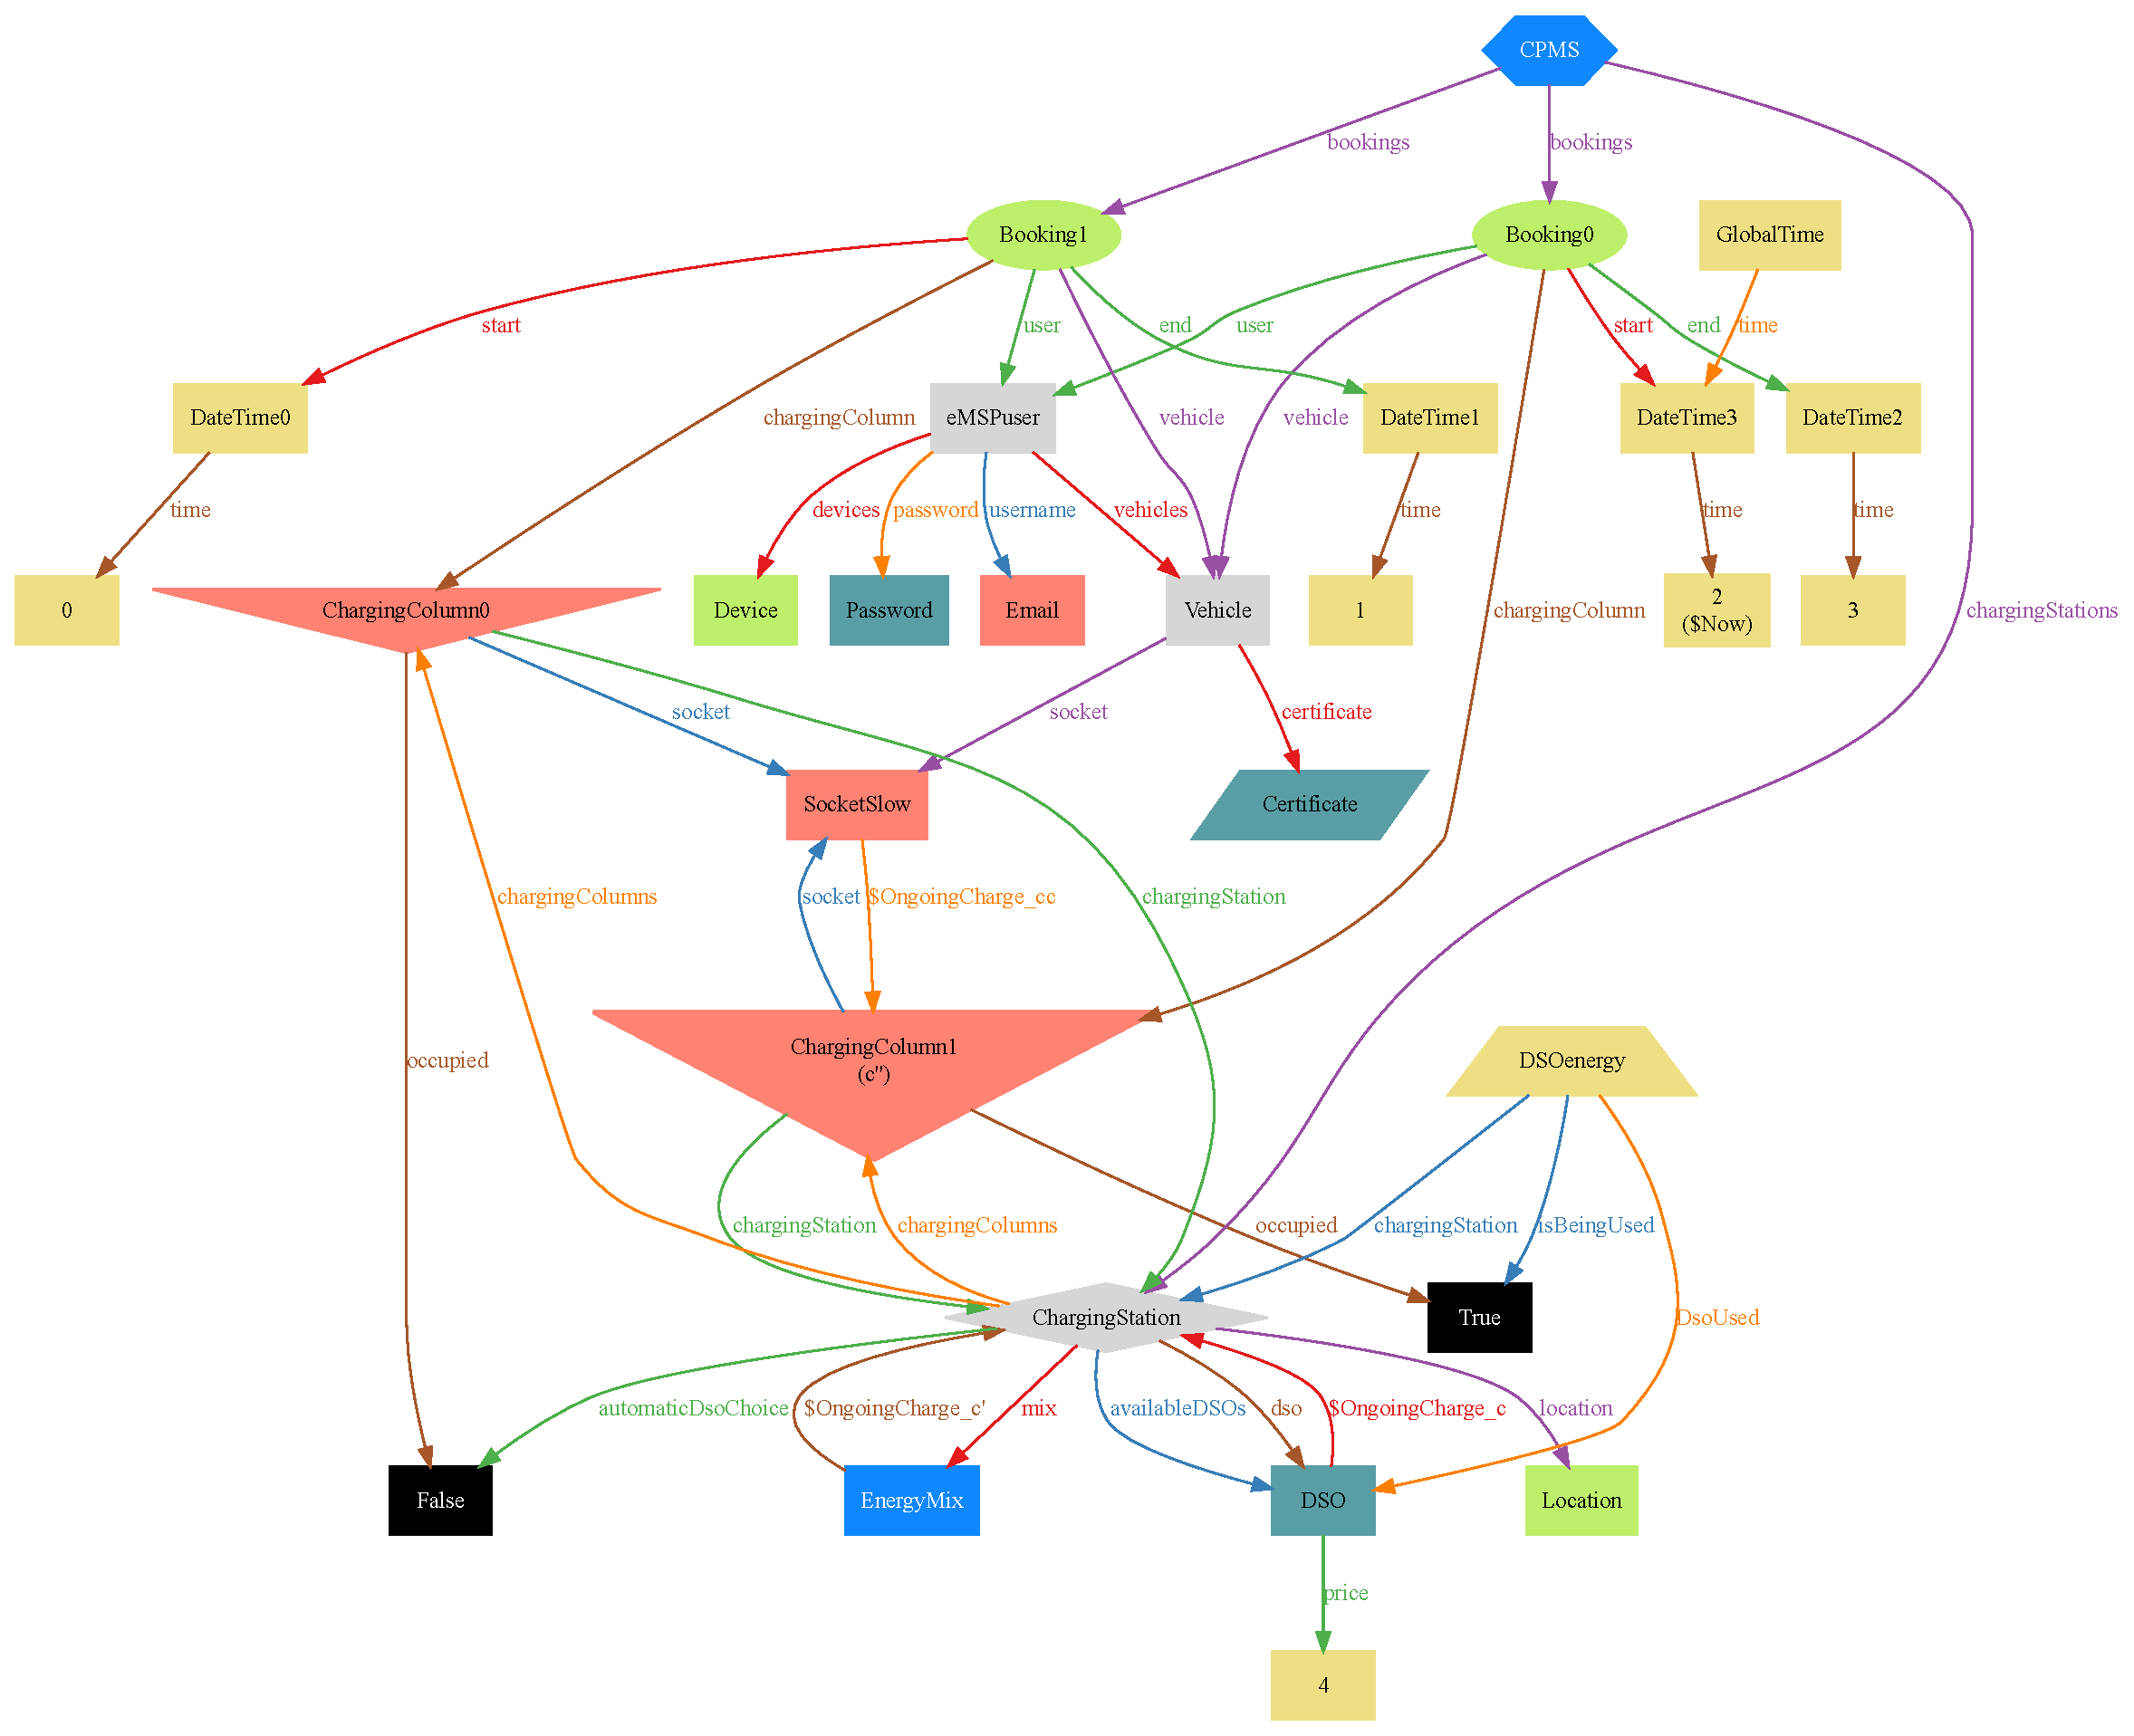
\includegraphics[width=\columnwidth]{./images/alloy/ongoingCharge}
    \caption{the ongoing charge of a vehicle at the charging column.}
\end{figure}

\pagebreak

\subsection{Creation of a booking}

This diagram shows the creation of the first booking by an eMSP user (which is not depicted here) at a specific charging station. The relative column is associated automatically by the system.

\begin{minted}{Alloy}
pred BookCharge[c, c': CPMS, b: Booking] {
    c'.users = c.users
    c'.chargingStations = c.chargingStations
    c'.bookings = c.bookings + b
    #Device = 0
    #ChargingColumn = 1
    #DSO = 1
    #eMSPuser = 1
    #CPMSuser = 0
}
\end{minted}

\begin{figure}[h!]
    \centering
    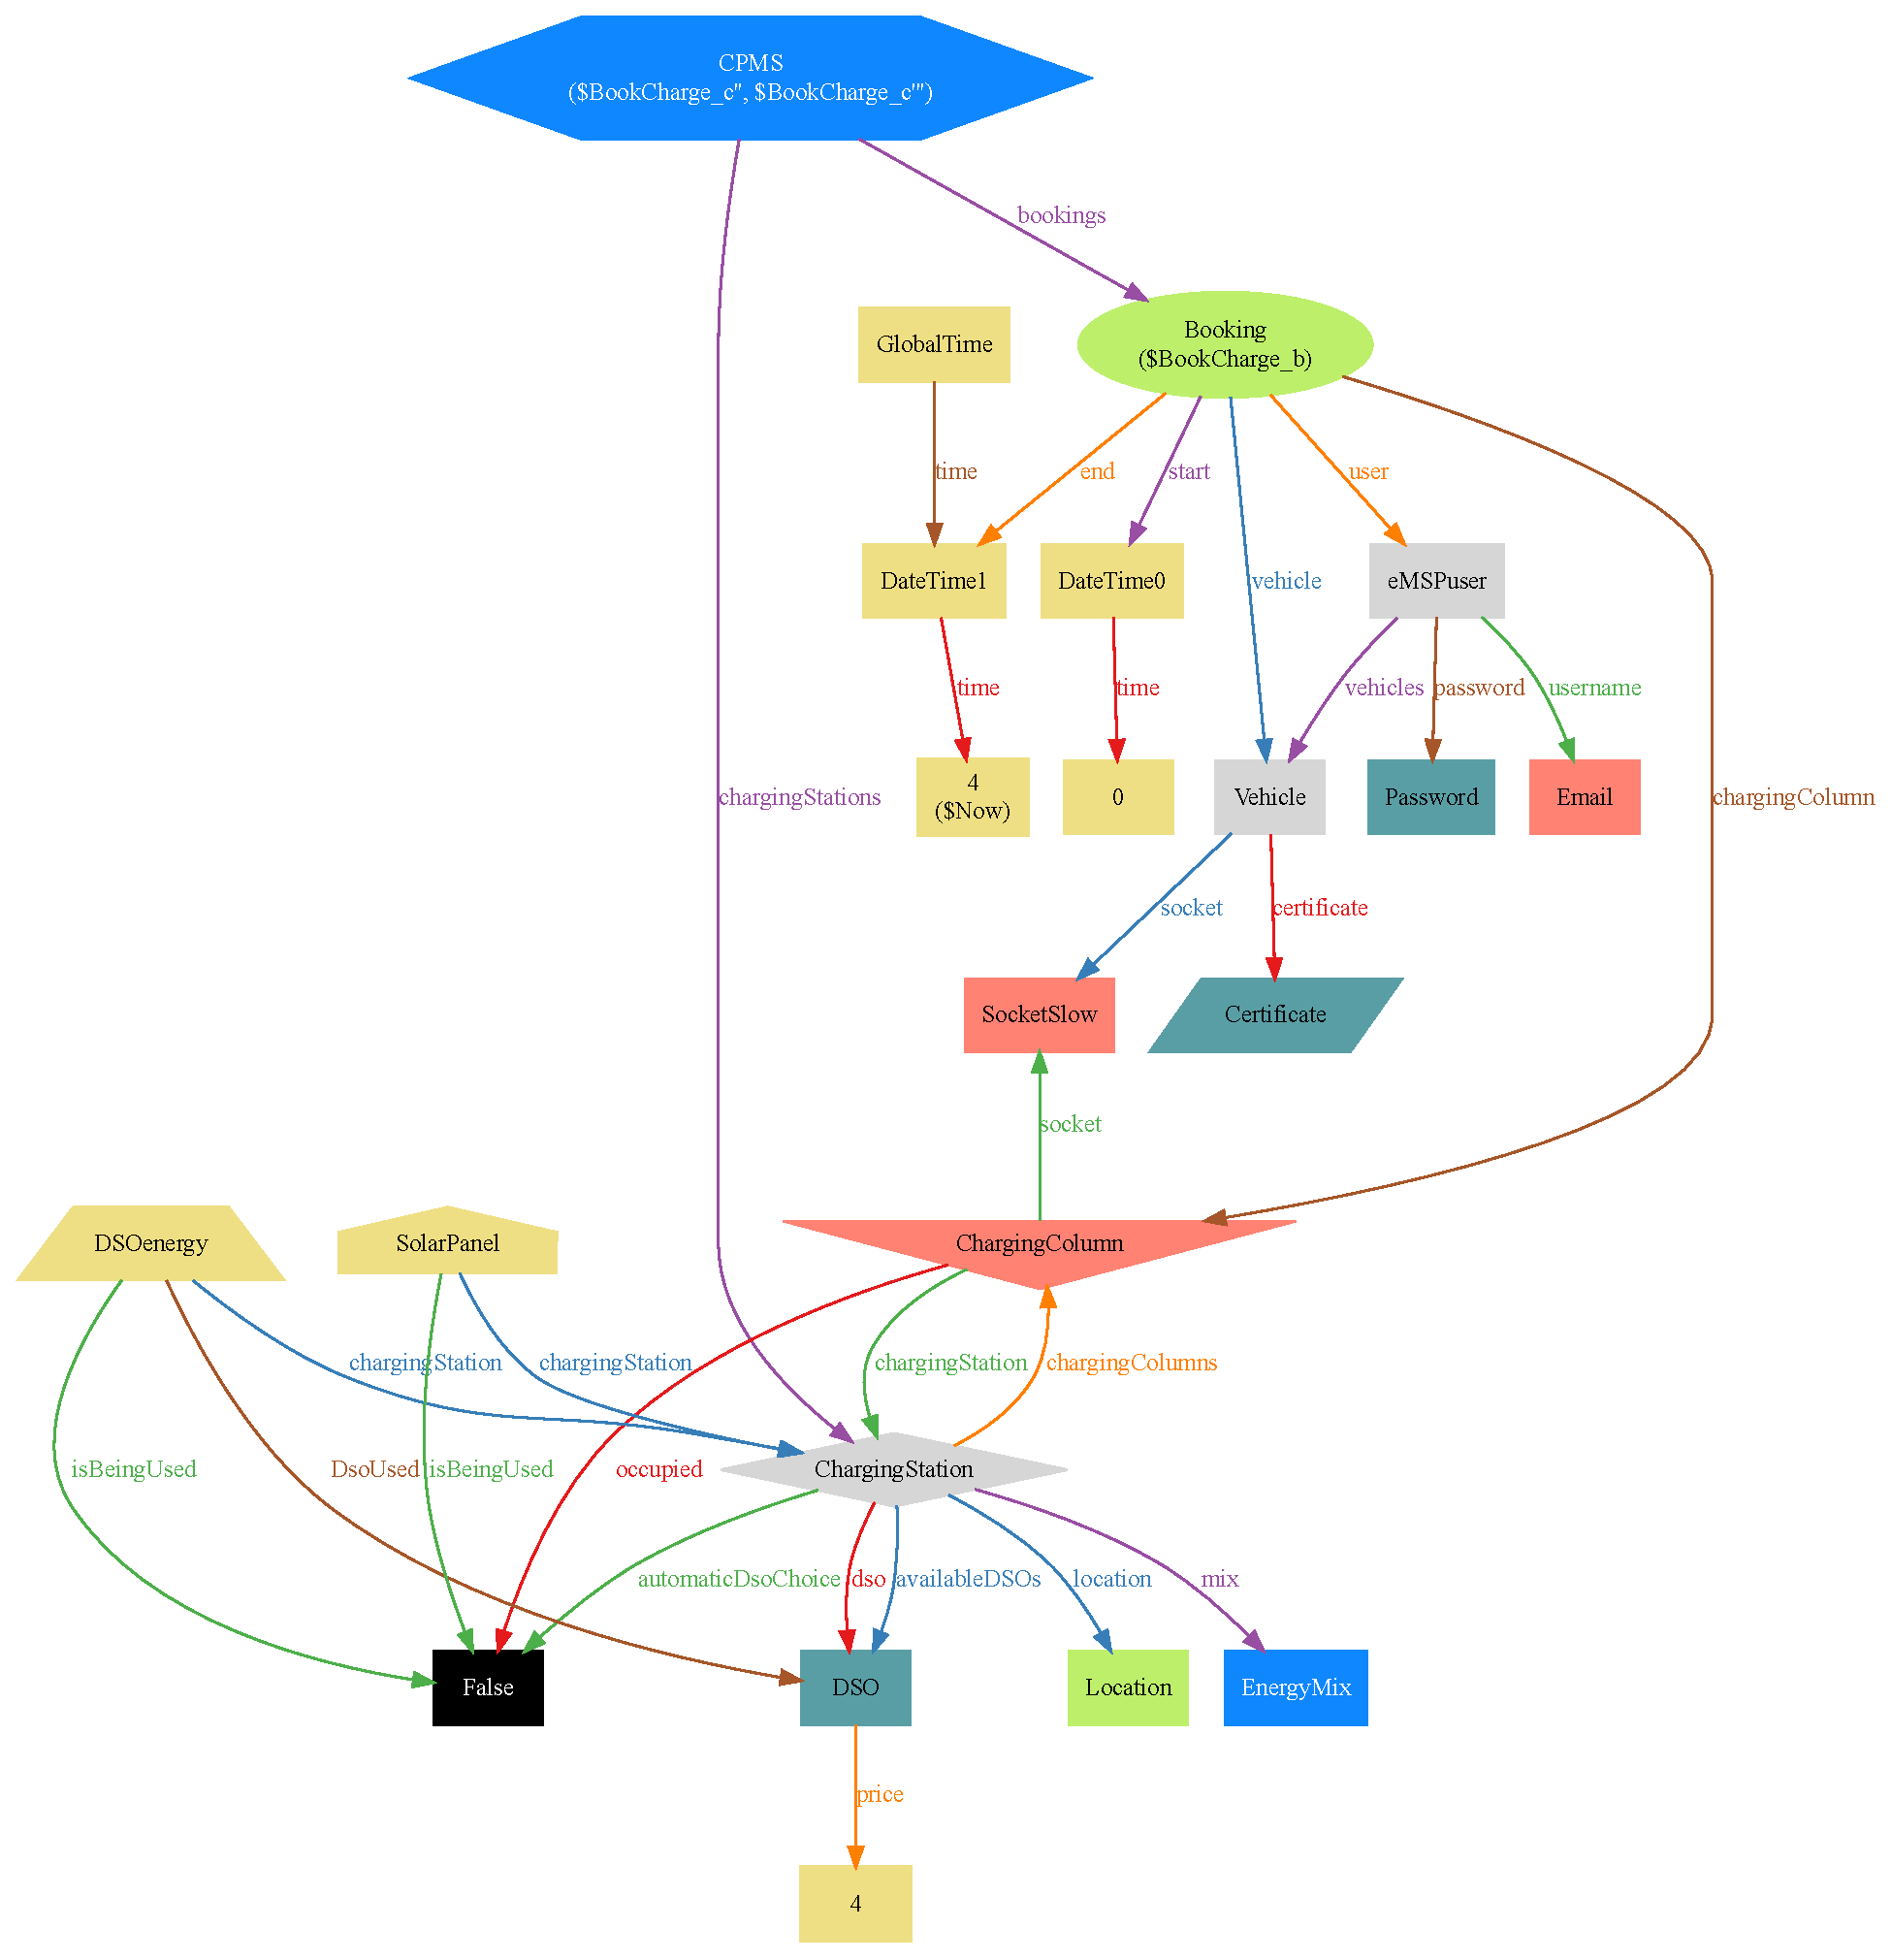
\includegraphics[width=\columnwidth]{./images/alloy/bookCharge}
    \caption{the creation of a new booking.}
\end{figure}

\pagebreak

\subsection{Addition of a vehicle}

This diagram shows the addition of a new vehicle by the eMSP user, connecting it to his account, thus making it available when booking a new charge.

\begin{minted}{Alloy}
pred AddVehicle[u, u': eMSPuser, v: Vehicle] {
    u'.username = u.username
    u'.password = u.password
    u'.devices = u.devices
    u'.vehicles = u.vehicles + v
    u'.favorites = u.favorites
    #GlobalTime = 0
    #CPMS = 0
    #Device = 1
    #Vehicle = 2
}
\end{minted}

\begin{figure}[h!]
    \centering
    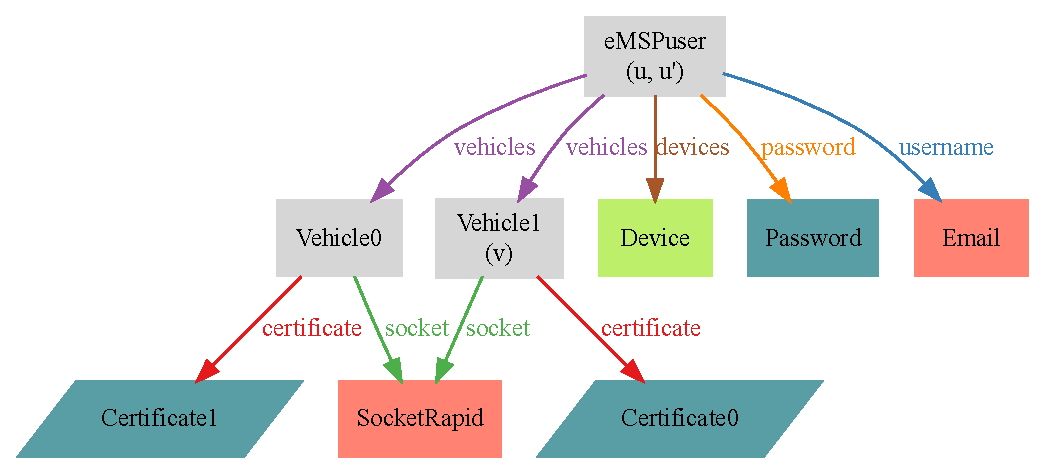
\includegraphics[width=0.5\columnwidth]{./images/alloy/vehicle}
    \caption{the addition of a new vehicle by the eMSP user.}
\end{figure}

\pagebreak

\subsection{Charging station sources}

This diagram shows that a charging station can have multiple energy sources, but that according to the energy mix, some of them may not be used at a specific point in time.

\begin{minted}{Alloy}
pred Sources {
    #eMSPuser = 0
    #CPMS = 1
    #CPMSuser = 0
    #ChargingStation = 1
    #EnergySource = 6
    #GlobalTime = 0
    some d: DSOenergy | d.isBeingUsed = False
}
\end{minted}

\begin{figure}[h!]
    \centering
    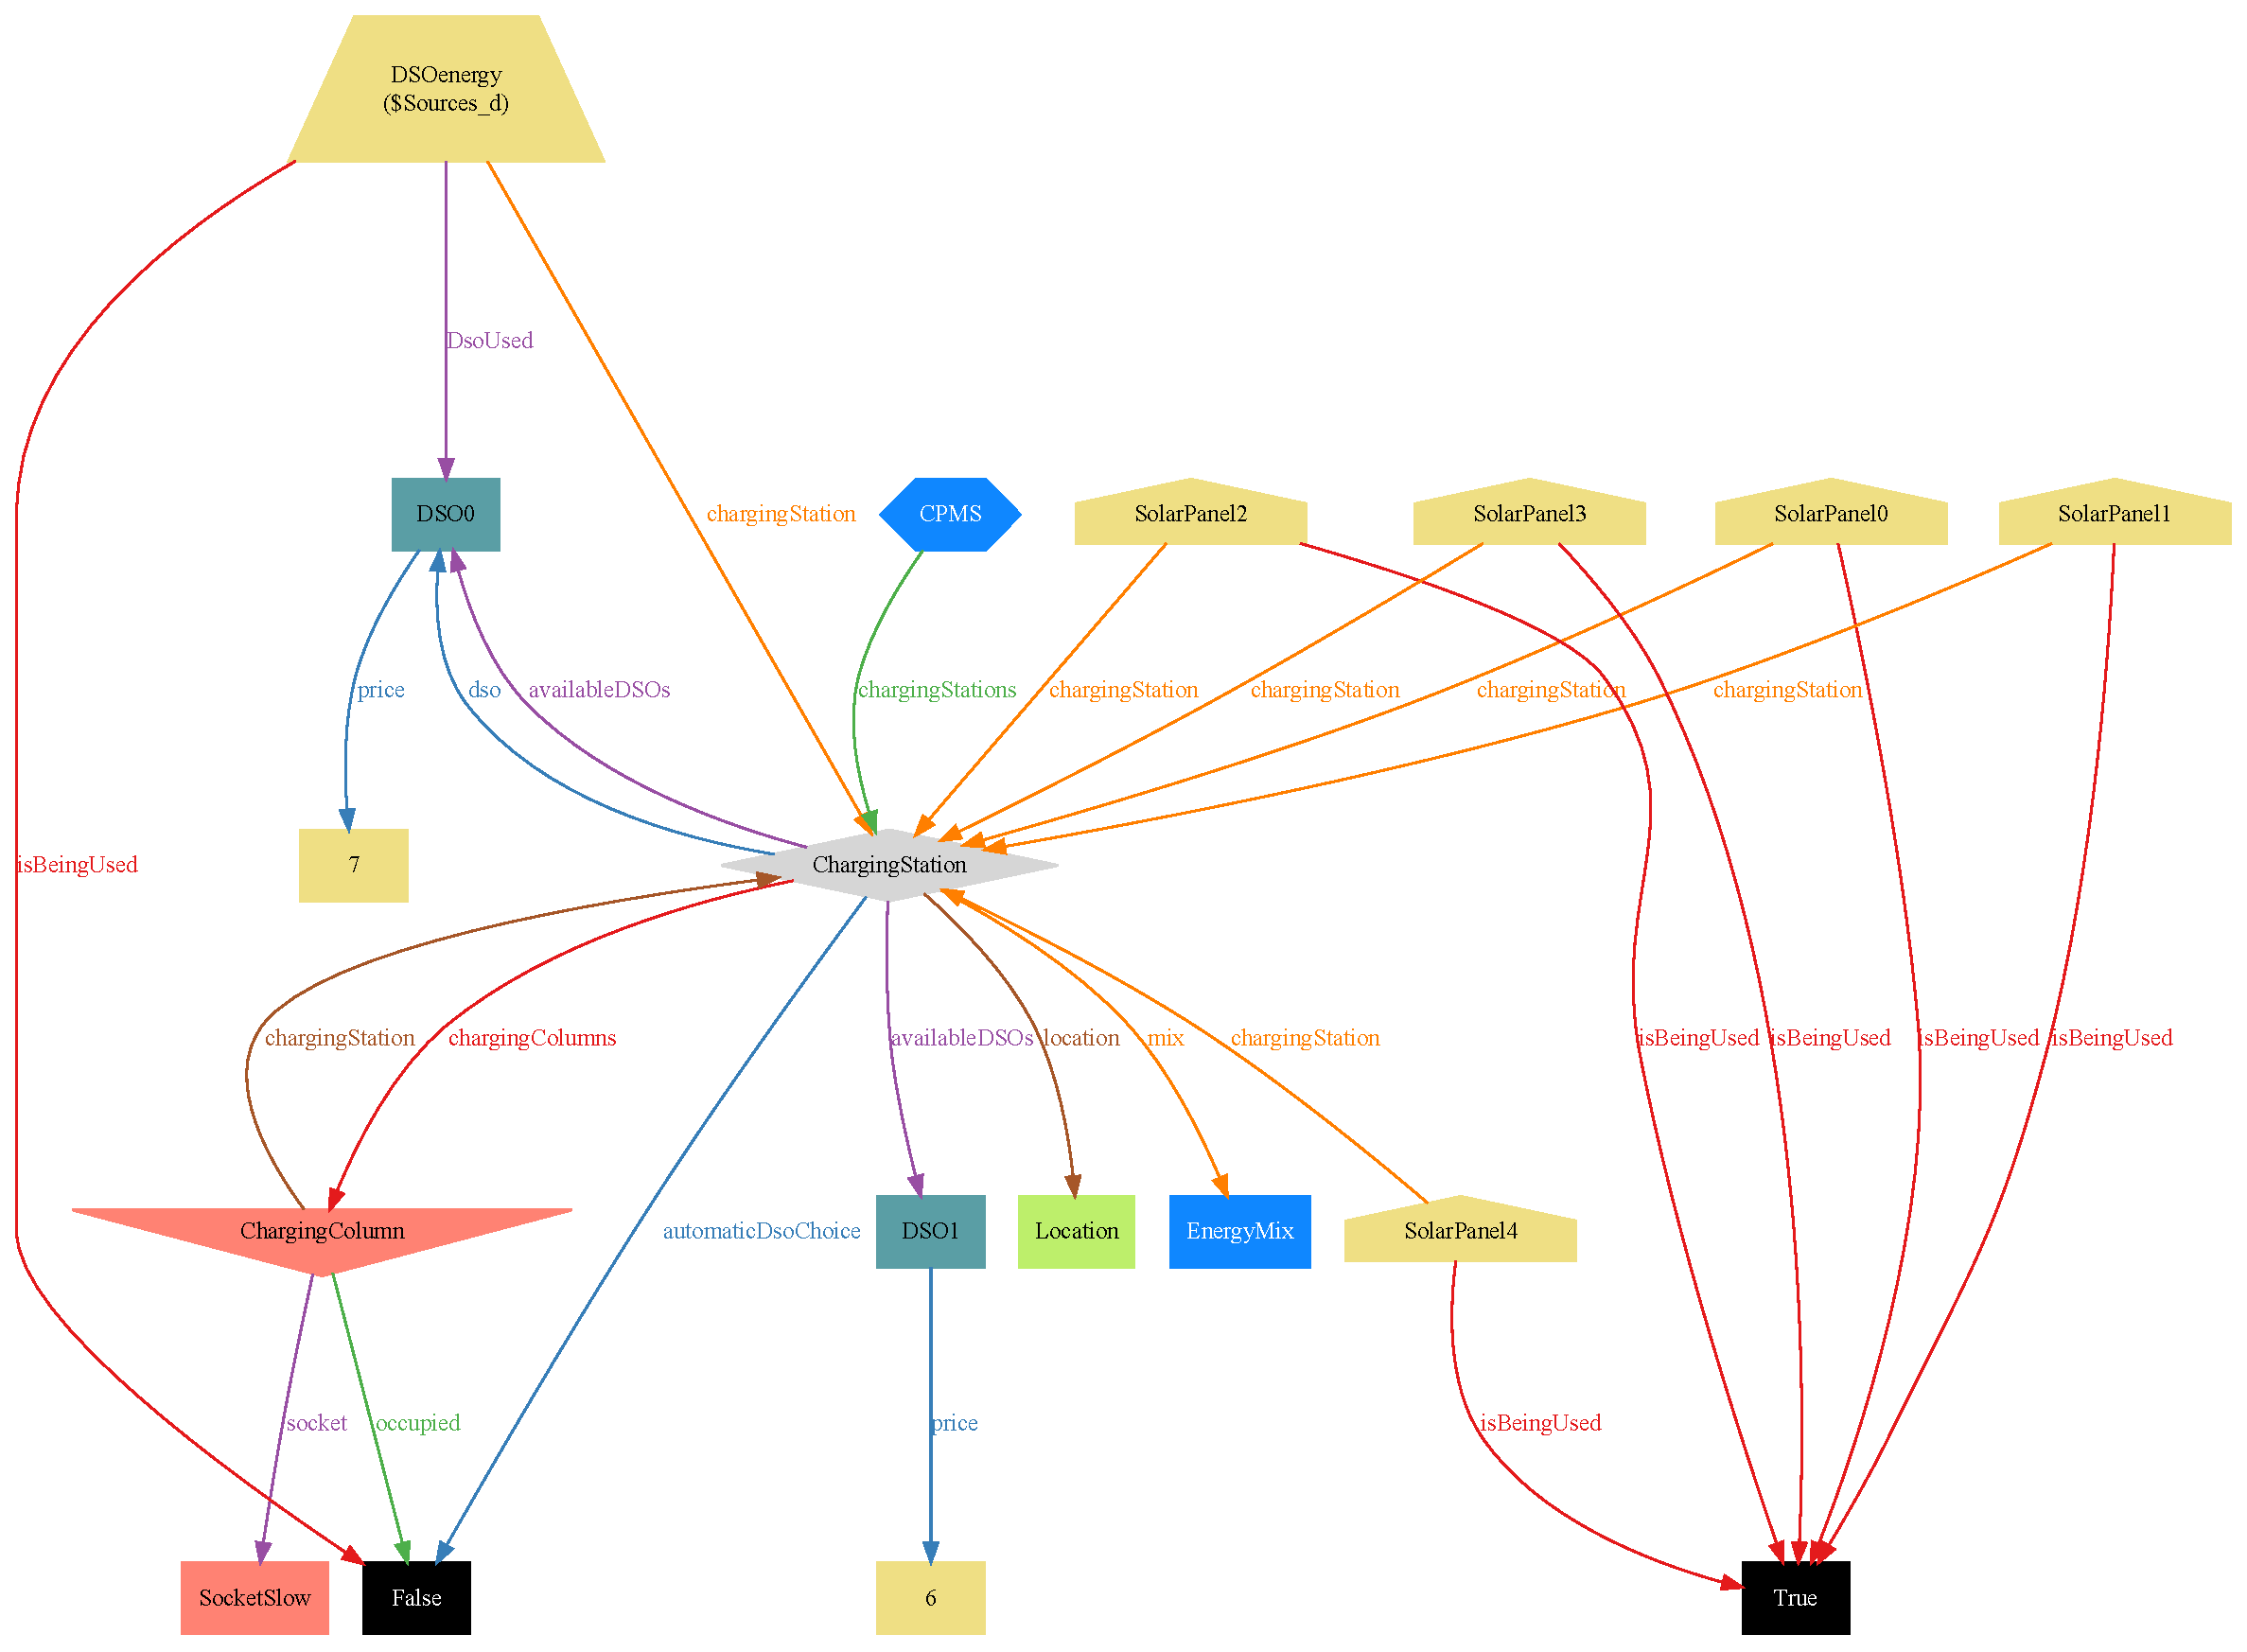
\includegraphics[width=\columnwidth]{./images/alloy/sources}
    \caption{the energetic situation at the charging station.}
\end{figure}

\pagebreak

\subsection{Automatic DSO choice}

This diagram shows the choice of a DSO from which buying the energy for supplying the charging stations which have in their energy mix the energy coming from the DSO.

\begin{minted}{Alloy}
pred AutomaticDSOChoice {
    #ChargingStation = 2
    #DSO > 2
    #eMSPuser = 0
    some cs: ChargingStation | cs.automaticDsoChoice = True
    some cs: ChargingStation | cs.automaticDsoChoice = False
    all cs: ChargingStation | #cs.availableDSOs > 1
}
\end{minted}

\begin{figure}[h!]
    \centering
    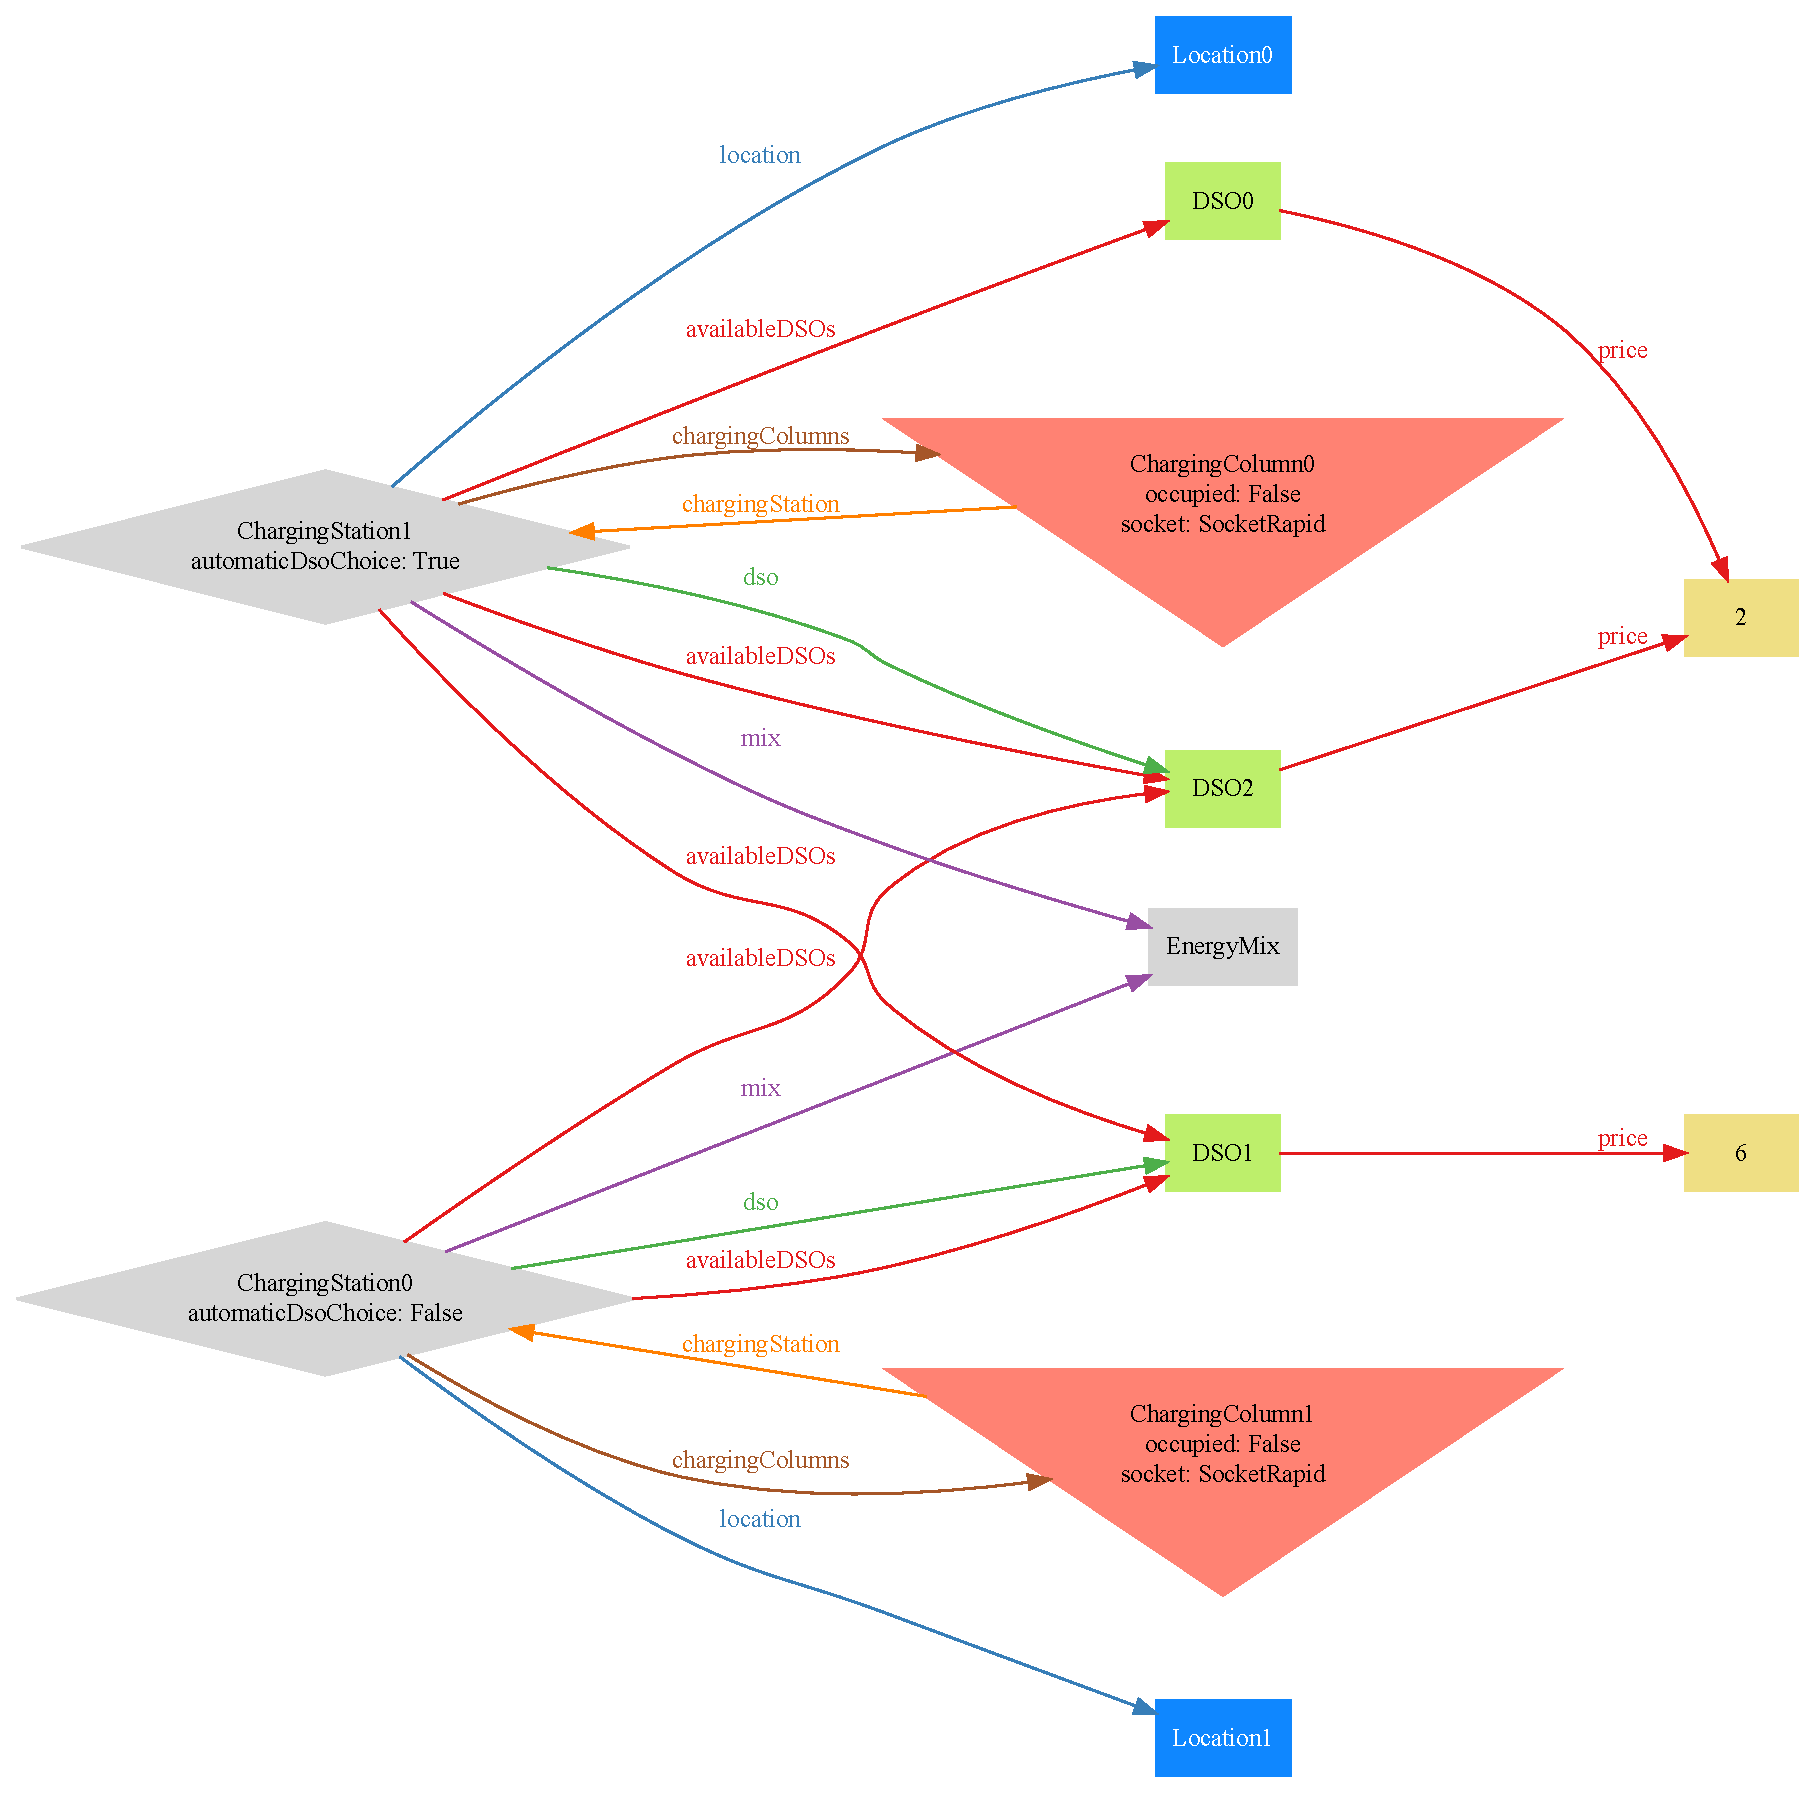
\includegraphics[width=\columnwidth]{./images/alloy/autoDSO}
    \caption{the automatic choice of a DSO.}
\end{figure}

\pagebreak

\subsection{A rather complete world}

This diagram shows a world which tries to be as complete as possible.

\begin{minted}{Alloy}
pred GenericWorld {
    #Email = 3
    #Password = 4
    #eMSPuser = 2
    #Vehicle >= 1
    #Device >= 1
    #CPMS = 1
    #CPMSuser = 2
    #ChargingStation >= 2
    #Booking >= 2
    #DSO >= 2
    #EnergySource >= 3
    no u: eMSPuser | #u.vehicles = 0
    some c: ChargingColumn | c.occupied = True
}
\end{minted}

\begin{figure}[h!]
    \centering
    
\includegraphics[width=\columnwidth]{./images/alloy/generic}
    \caption{a generic, but rather complete, world.}
\end{figure}

    \chapter{Conclusions} \label{conclusions}

\section{Final thoughts}

This document was redacted following the guidelines for the project (\textit{eMall - e-Mobility for All project}). Discrepancies between our document and the guidelines are to be considered our hypothesis on how the two systems should behave or be modeled.\medskip

Also, these systems have been designed having in mind possible future expansions. Thus, anyone who wants to expand this project is welcome and encouraged to do so.

\section{Credits} \label{credits}

For writing this document, we used different pieces of software from the Internet. This is a rather comprehensive list of them:
\begin{itemize}
    \item \href{https://www.latex-project.org/}{\textit{\LaTeX} (with packages)} and \href{https://code.visualstudio.com/}{\textit{Visual Studio Code} (with plugins)} for writing the document.
    \item \href{https://git-scm.com/}{\textit{Git}}, \href{https://github.com/}{\textit{GitHub}} and \href{https://www.notion.so/}{\textit{Notion}} for keeping things organized.
    \item \href{https://www.diagrams.net/}{\textit{draw.io}} and \href{https://plantuml.com/}{\textit{PlantUML}} for creating the diagrams.
\end{itemize}

\section{Effort}

\begin{center}
    \begin{tabular}{ | >{\arraybackslash}m{0.52\columnwidth} | >{\centering\arraybackslash}m{0.2\columnwidth} | >{\centering\arraybackslash}m{0.2\columnwidth} | }
        \hline
        \multicolumn{1}{|c|}{\textbf{Task}} & \textbf{Riccardo Motta} & \textbf{Pierluigi Negro} \\
        \hline
        \hline
        Starting off & 1h & 2h \\
        \hline
        Defining goals and phenomena & 2h & 2h \\
        \hline
        Defining scenarios, functions, users, and domain assumptions & 3h & 3h \\
        \hline
        Creating class diagram & 3h & 2.5h \\
        \hline
        Defining requirements & 2h & 2h \\
        \hline
        Goal mapping & 2h & 2h \\
        \hline
        Creating use cases & 8h & 6h \\
        \hline
        Alloy writing & 10.5h & 10.5h \\
        \hline
        Document writing & 16h & 17h \\
        \hline
        Updating document for Version 1.1 & 0.5h & 0h \\
        \hline
        \hline
        \textbf{Total} & \textbf{48h} & \textbf{47h} \\
        \hline
    \end{tabular}
\end{center}


\end{document}
